\section{Mapas Cuadráticos 2-D Implementados en Punto Fijo}
\label{sec:StochDegr}

En esta Sección se emuló el comportamiento de una implementación en hardware digital, como FPGA, dispositivo lógico programable complejo (CLPD) o circuito integrado de aplicaciones específicas (ASIC), para replicar exactamente el funcionamiento del dispositivo.
Nuestro interés es medir cómo los dominios de atracción se degradan en función del número de bits $n$ empleado, y así encontrar el valor umbral $n_{min}$ para el cual se conservan ciertas propiedades estadísticas requeridas.

El trabajo de Grebogi \cite{Grebogi1988} mostró que la longitud promedio de las órbitas periódicas $T$ de un sistema dinámico implementado en una computadora, escala en función de la precisión de la computadora $\xi$ y la dimensión de correlación $D$ del atractor caótico, como $T \sim \xi ^ {- D / 2}$.
En este caso el objetivo es investigar las características de cada precisión para que el diseñador tenga una visión general completa de las opciones que se utilizarán en su implementación.
De esta manera, se podrán establecer las propiedades a rescindir según los requerimientos y los recursos disponibles al momento del diseño.

Además de analizar los cambios en las duraciones de los períodos, las propiedades estadísticas de las secuencias serán diferentes de las del sistema real, por lo que también deberían analizarse.
En \cite{Persohn2012} se desarrolló un excelente trabajo sobre las consecuencias que tiene la precisión finita sobre la periodicidad de un PRNG basado en el mapa Logístico.
Allí, se determinaron el número, retardo y período de las órbitas del mapa Logístico con diversos grados de precisión, sin embargo, este trabajo carece de un análisis estadístico.
La investigación realizada en este Capítulo complementa su trabajo al agregar cuantificadores estadísticos.
Además aquí se estudia la implementación en arquitectura de punto fijo (en cambio en \cite{Persohn2012} se utilizó punto flotante) ya que es la arquitectura que menos recursos emplea en las implementaciones en hardware.
Como consecuencia, el consumo de energía también se ve disminuido.

Entre muchos sistemas caóticos disponibles en la literatura, se utilizó la familia de mapas cuadráticos bidimensionales descriptos en la Sección \ref{ssecQMaps}.
Solo los resultados para la representación analítica de los mapas en \cite{Sprott1993} han sido publicados en la literatura abierta.

El objetivo en esta Sección es ampliar el análisis a la versión digital para posibilitar la implementación del hardware en aritmética de punto fijo, para lo cual es imprescindible conocer la duración del período y el grado de aleatoriedad de las secuencias generadas por el sistema discretizado.
Se desarrolló un análisis detallado de la \textsl{degradación} del sistema caótico multiatractor a medida que varía la precisión empleada en una implementación de punto fijo.
Por \textsl{degradación} se entiende:
(a) la aparición de puntos fijos estables y órbitas periódicas estables con períodos cortos, dentro de un dominio de atracción de coma flotante sin órbitas estables;
(b) el mismo atractor se vuelve periódico y sus características estadísticas cambian, lo que hace que el sistema sea más determinista.

Las principales contribuciones de esta Sección son:
\begin{itemize}
	\item el análisis de los dominios de atracción de los atractores caóticos para un conjunto dado de parámetros a medida que aumenta el número de bits; en términos de la duración del período y la aparición de puntos fijos estables y órbitas periódicas con períodos cortos;
	\item la determinación del consecuente umbral para el ancho del bus, para hacer que las propiedades estadísticas de la implementación digital sean cercanas a las de la implementación de coma flotante;
	\item se asignan dos PDFs distintas para evaluar la estocasticidad de la serie temporal para diferentes anchos de bus.
	Cada PDF $P$ se mide por la correspondiente entropía de Shannon normalizada $H(P)$.
	Estas entropías tienen cambios abruptos en anchos de bus específicos.
	Las duraciones de los períodos y el \textsl{MLE} también se evalúan y los resultados se comparan con las $H(P)$.
\end{itemize}

\subsection{Resultados}

Un código ANSI C que simula un sistema no lineal iterando (el mapa cuadrático) en un dispositivo electrónico digital fue desarrollado con el fin de generar secuencias que luego fueron analizadas.

Este código itera el mapa cuadrático-$2D$ $10 ^ 5$ veces, en este caso los coeficientes $a_0$ a $a_ {11}$ tienen los valores: $\{a_i \}$ $=$ $\{- 1.0,$ $0.9,$ $0.4,$ $-0.2,$ $-0.6,$ $-0.5,$ $0.4,$ $0.7,$ $0.3,$ $-0.5,$ $0.7,$ $-0.8 \}$.
El sistema fue diseñado para trabajar en arquitectura fraccionaria de punto fijo con $n$ bits, donde $n = n_i + n_f$, en representación de complemento a $2$ ($Ca_2$).
En este caso, se empleó $n_i = 4$ bits para representar la parte entera, y el código varía automáticamente la cantidad de bits que representan la parte fraccionaria del número, $n_f$, para analizar cómo reacciona el sistema cuando cambia la precisión.
El código se ejecuta a partir de todas las CIs dentro del intervalo $[-2,2]$ en pasos determinados por $n_f$, por lo tanto, la grilla tendrá un paso de:
%
\begin{equation}
step\_grid=\frac{1}{n_f.2^{n_f}}.
\end{equation}

En cada caso se determinó si los sistemas evolucionan a un punto fijo, divergen o van hacia un ciclo periódico, también se generaron secuencias para esa misma CI usando diferentes $n_f$ bits de precisión.
Estos datos fueron luego evaluados utilizando los cuantificadores de aleatoriedad introducidos en la Sección \ref{capCuanti}.

La Figura \ref{fig:avvelo} muestra los dominios de atracción obtenidos para $n_i = 4$ y diferentes valores de $n_f$.
Los ejes de abscisas y ordenadas corresponden a valores iniciales de $x$ e $y$ respectivamente.
Cada punto representa una CI y el color está asociado a su estado final, mientras más oscuro es el tono de gris, más corto es el ciclo al que converge, los puntos fijos están en negro y los puntos divergentes en blanco.
Entonces, se pueden ver los diferentes dominios de atracción (incluyendo los atractores) que coexisten en el sistema para cada precisión.
%
\begin{figure*}
	\centering
	\begin{tabular}{cc}
		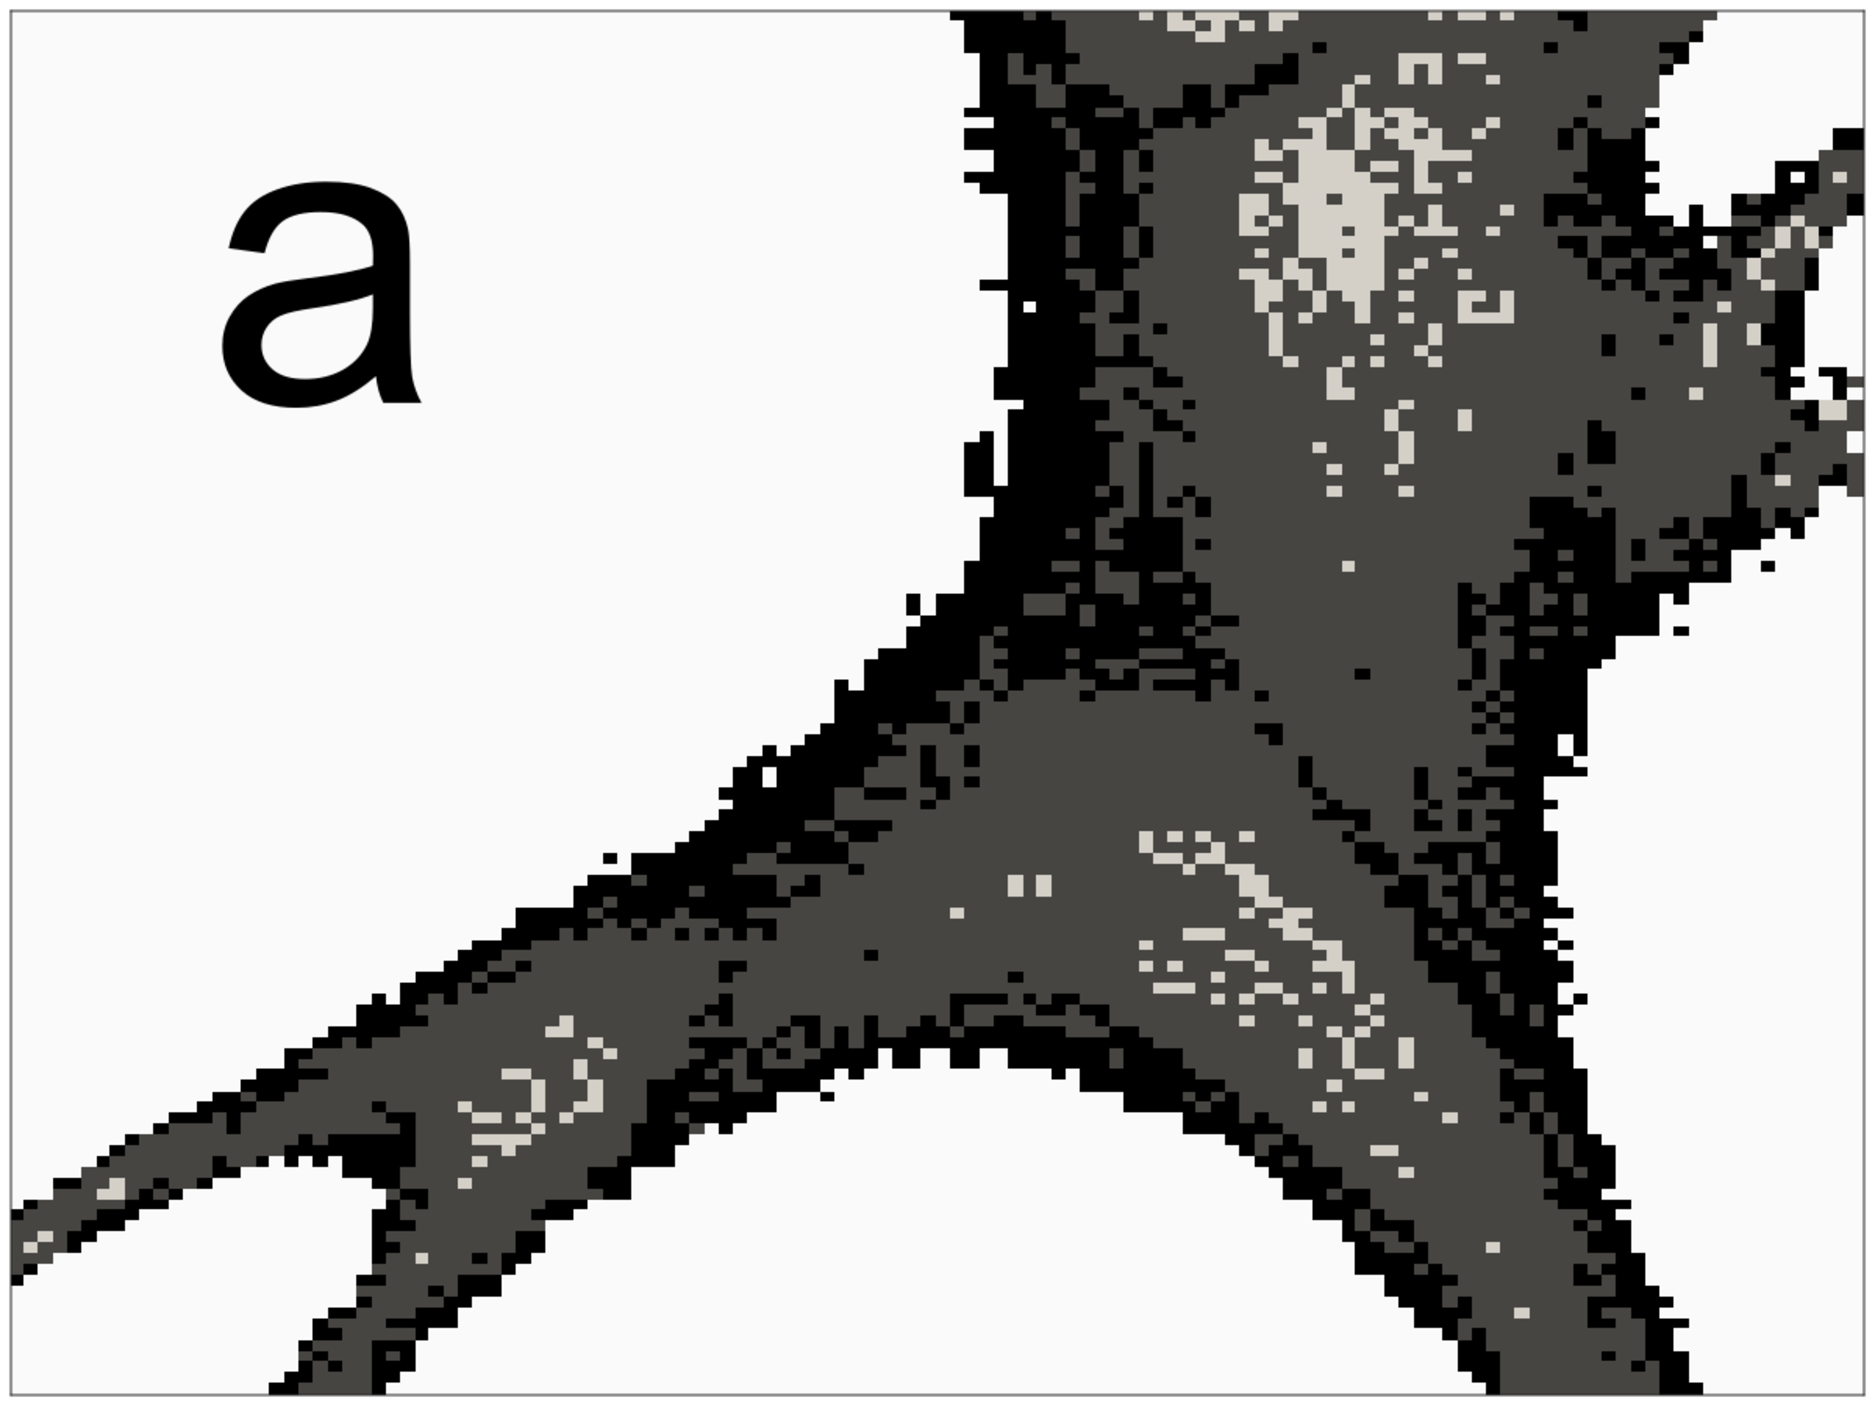
\includegraphics[width=0.32\textwidth]{m5_lu}
		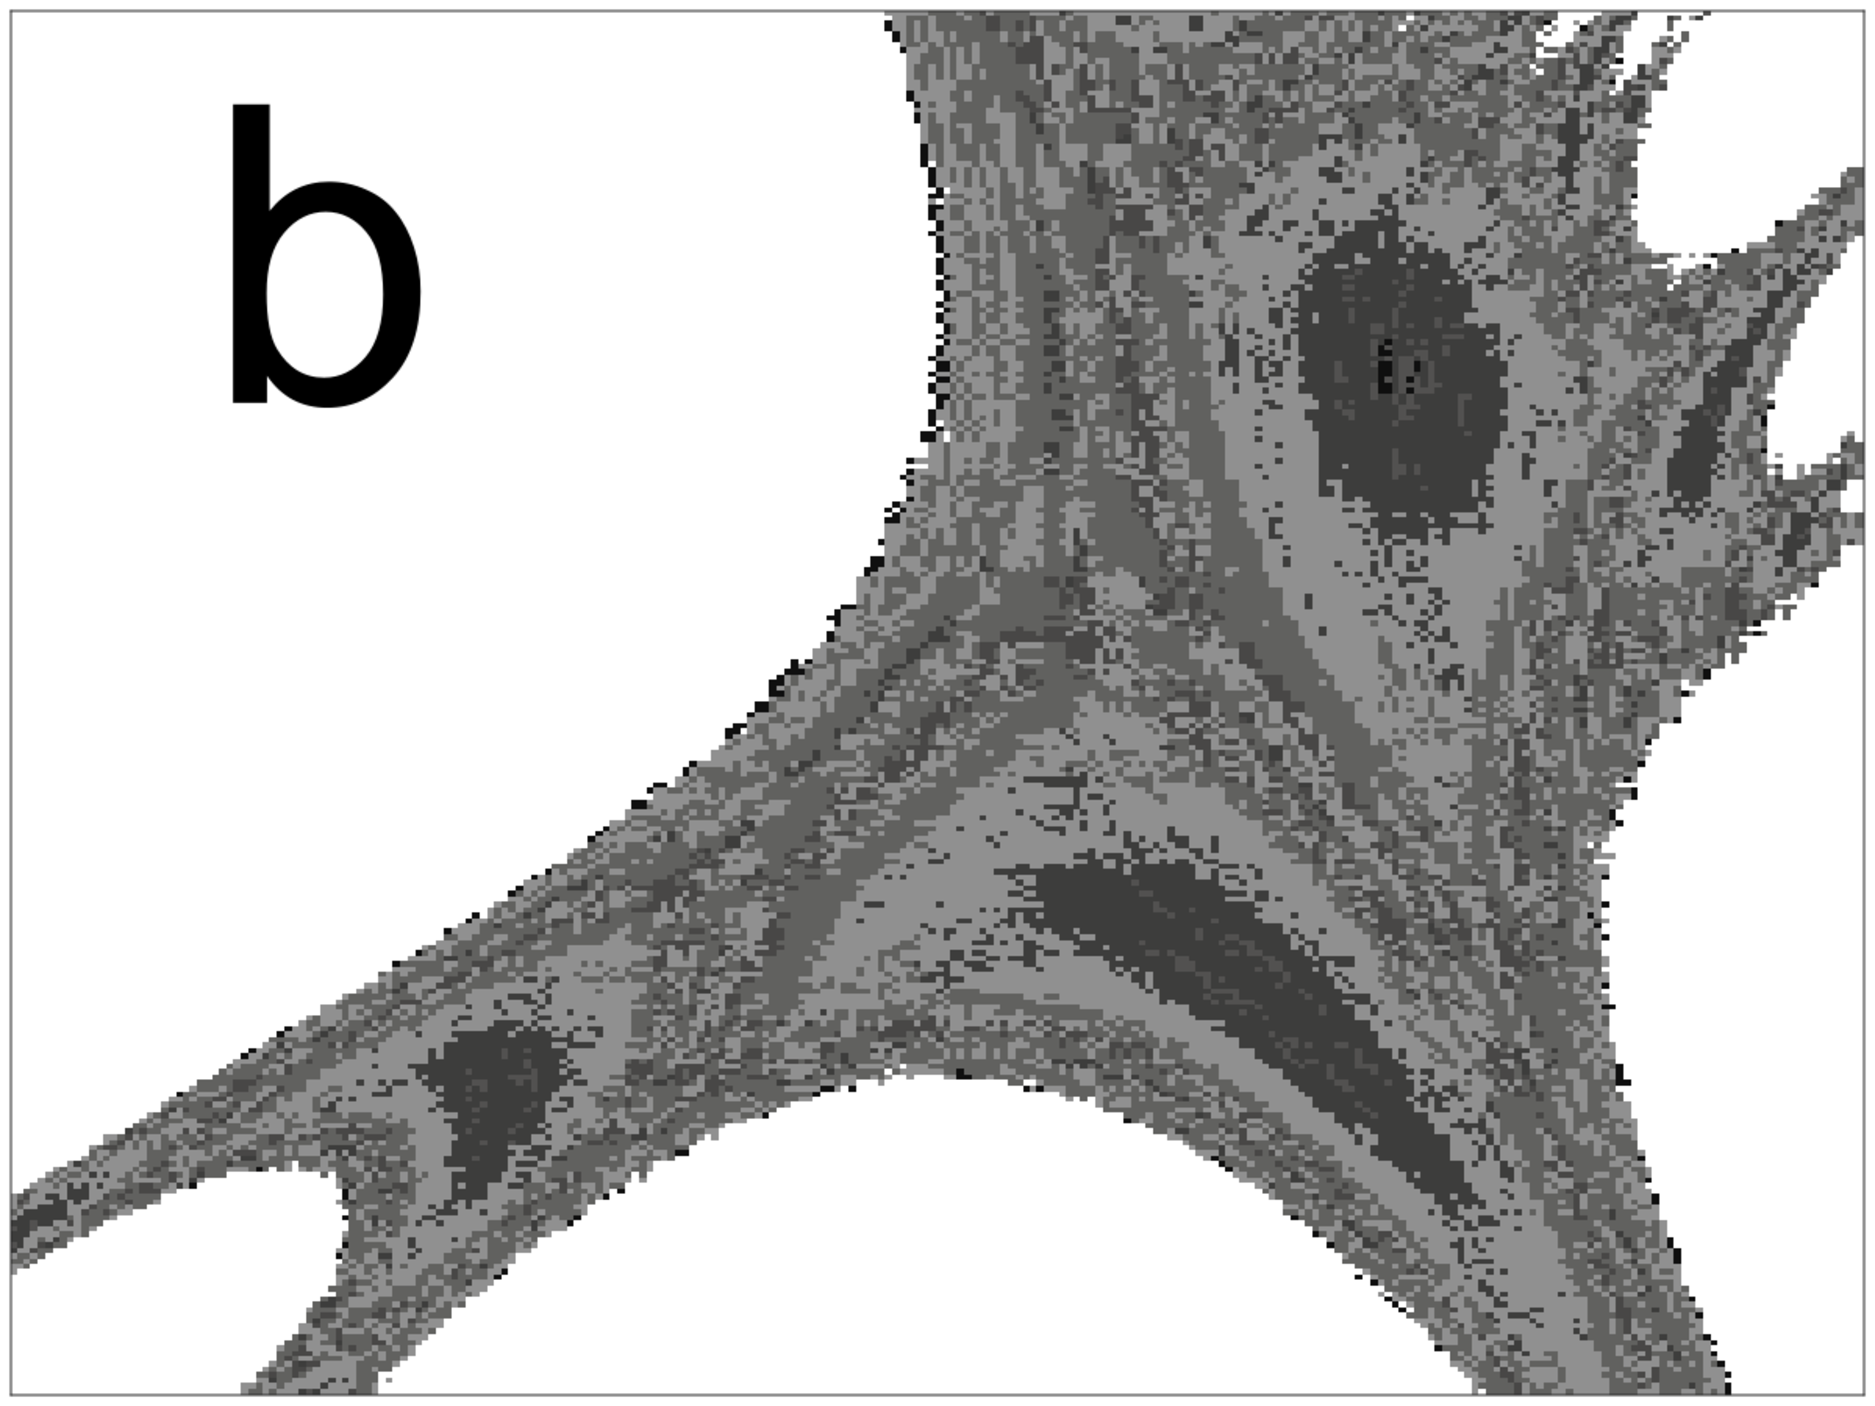
\includegraphics[width=0.32\textwidth]{m6_lu}
		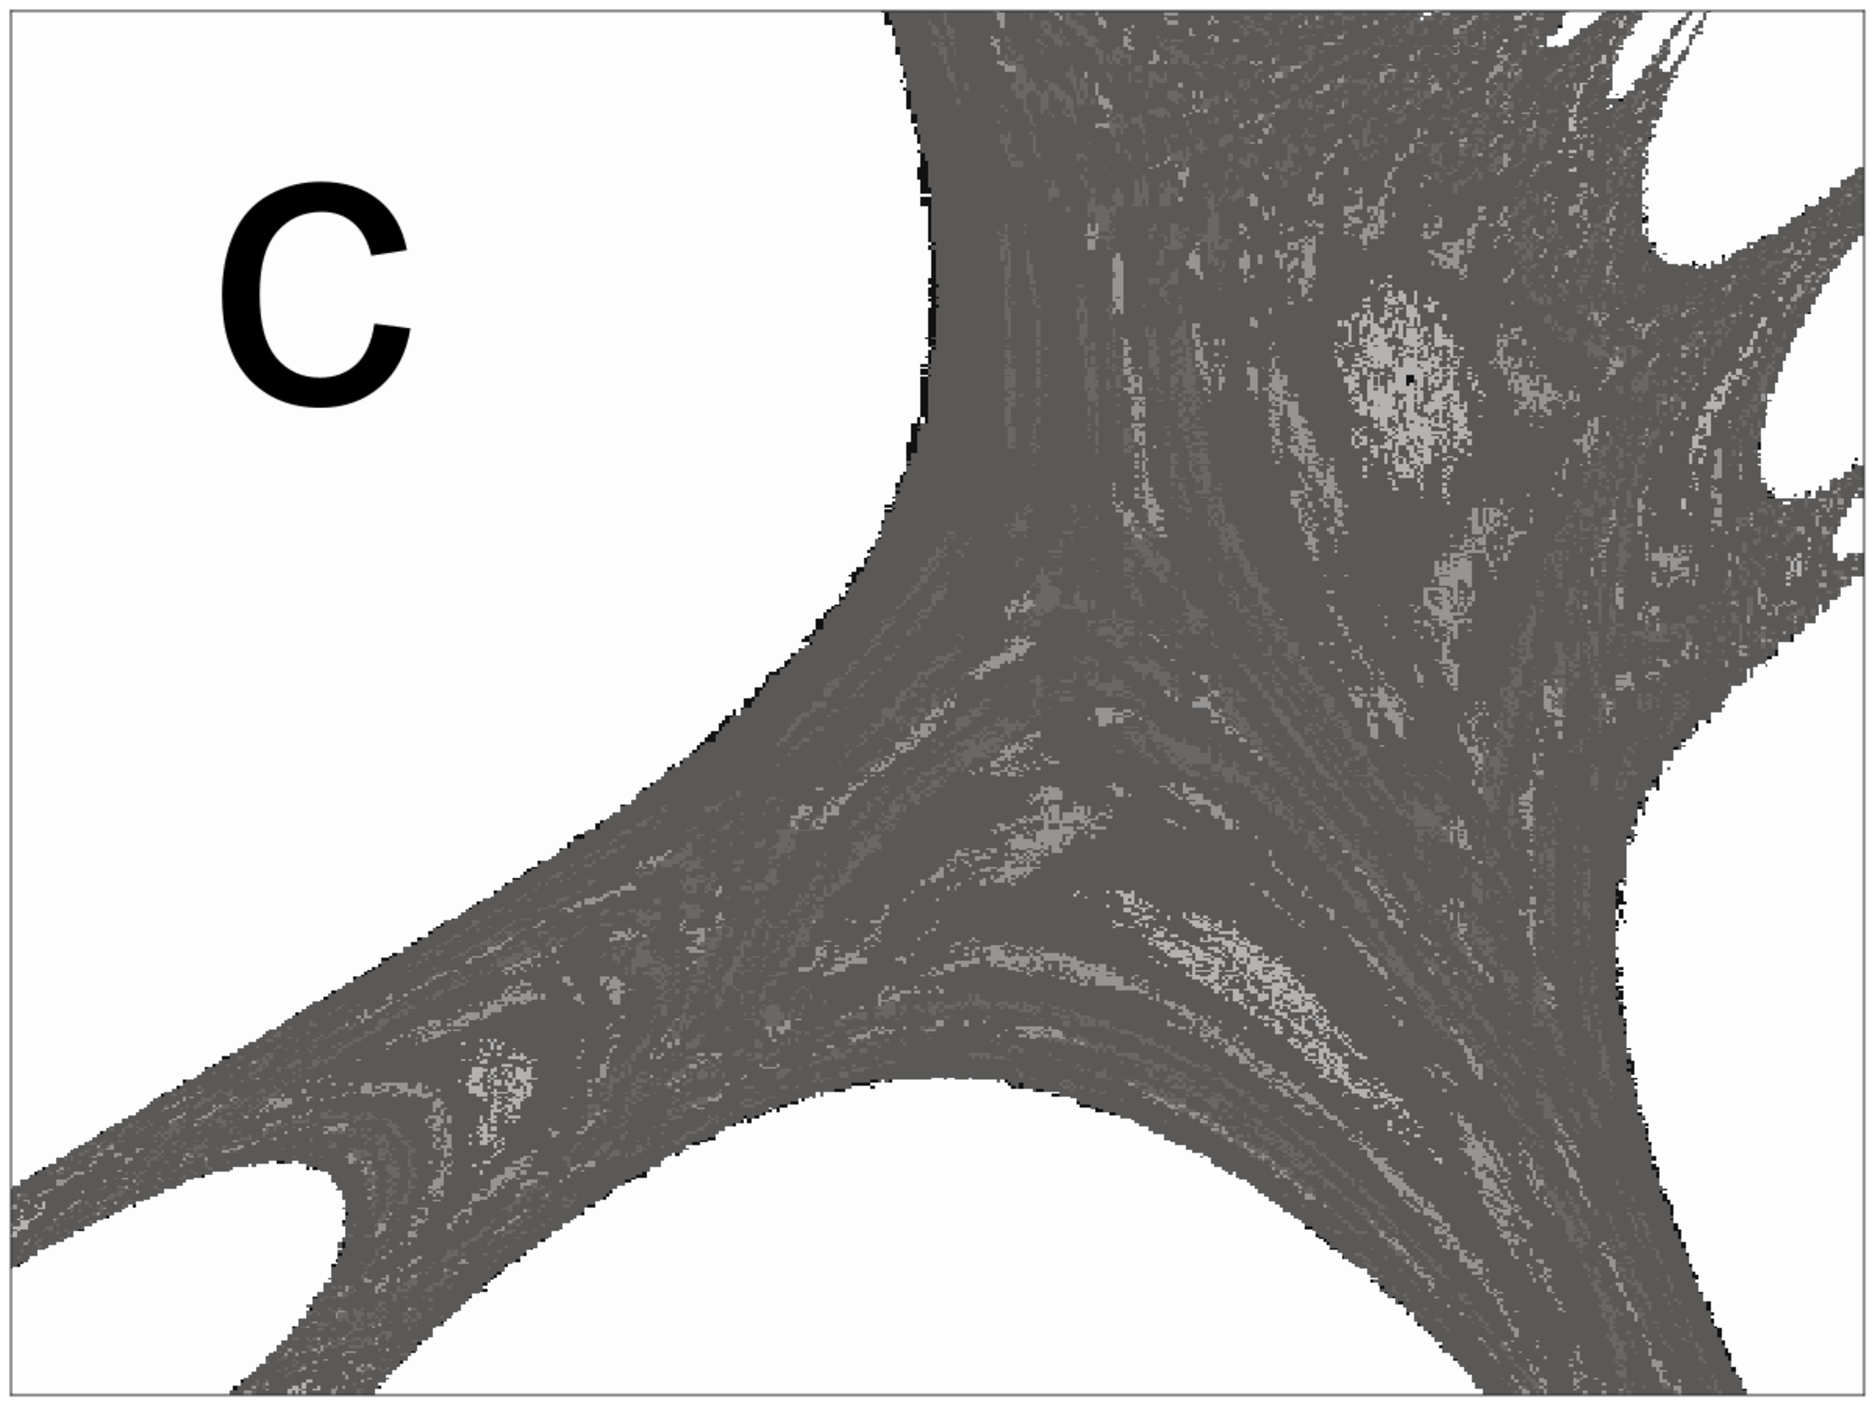
\includegraphics[width=0.32\textwidth]{m7_lu}\\
		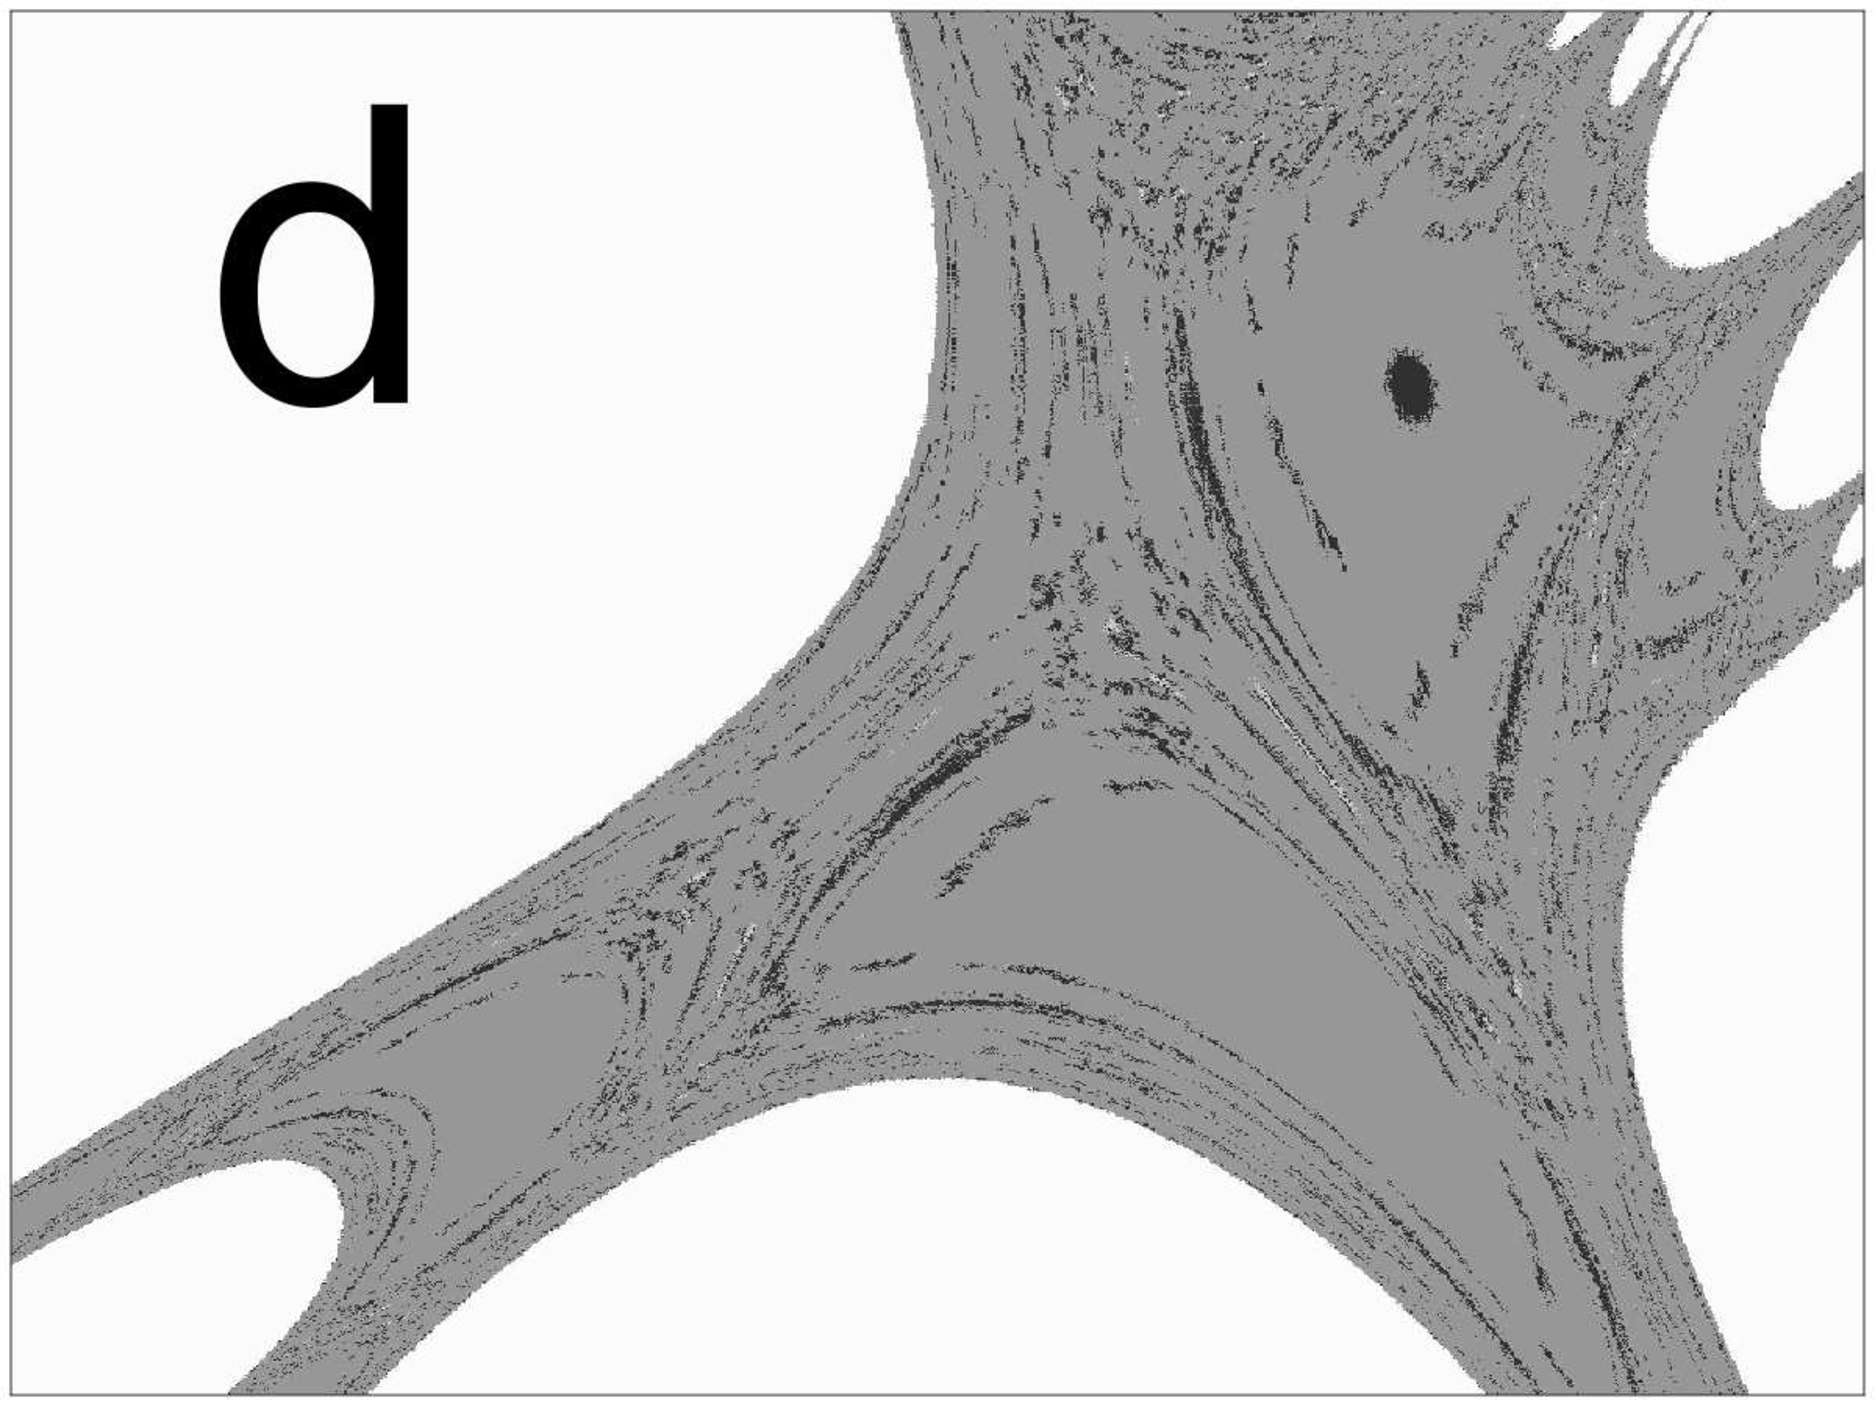
\includegraphics[width=0.32\textwidth]{m8_lu}
		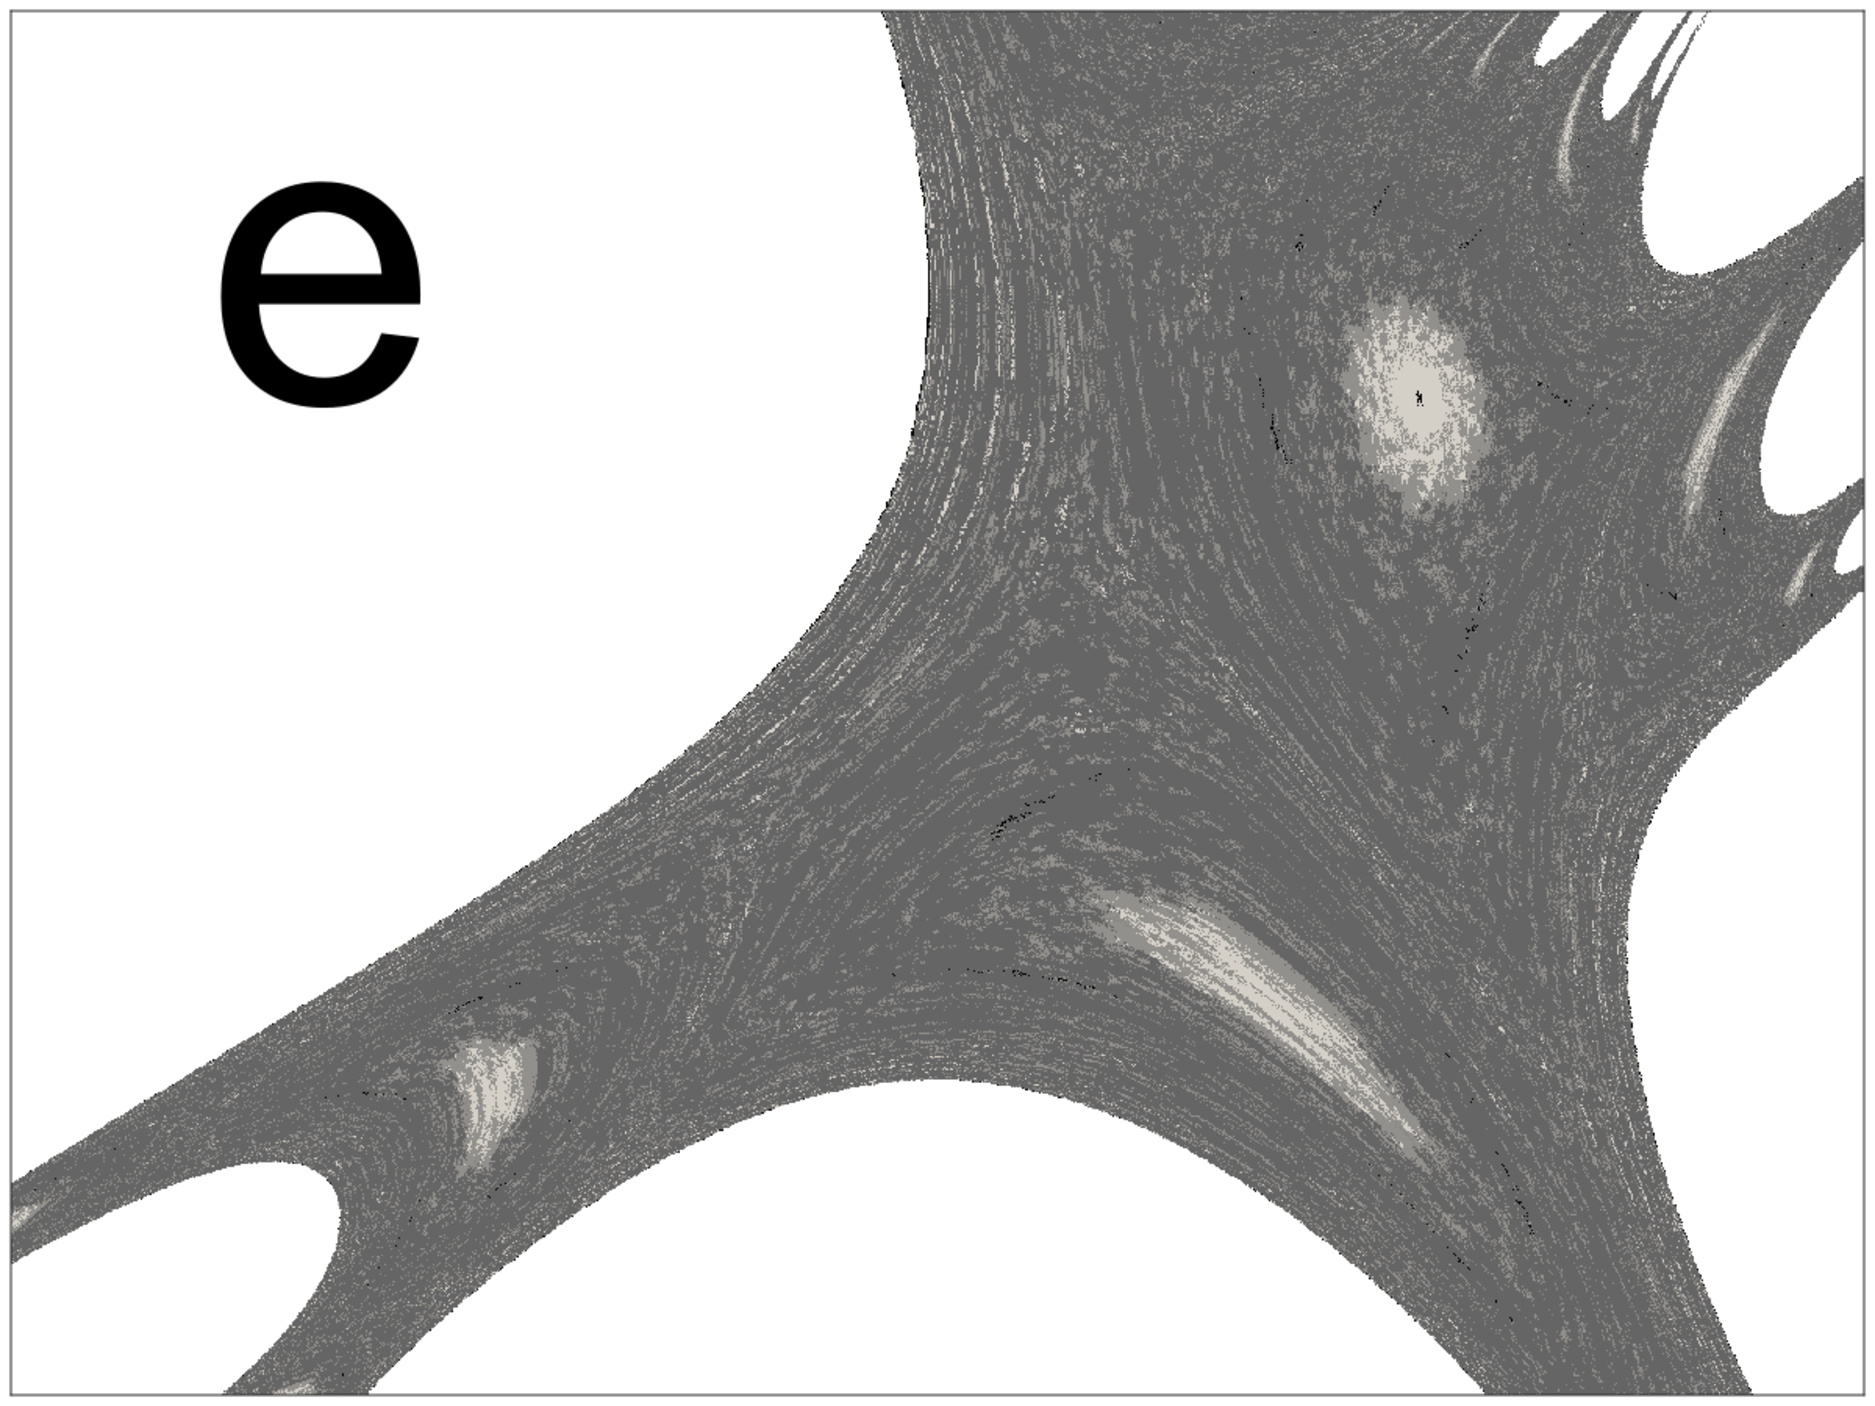
\includegraphics[width=0.32\textwidth]{m9_lu}
		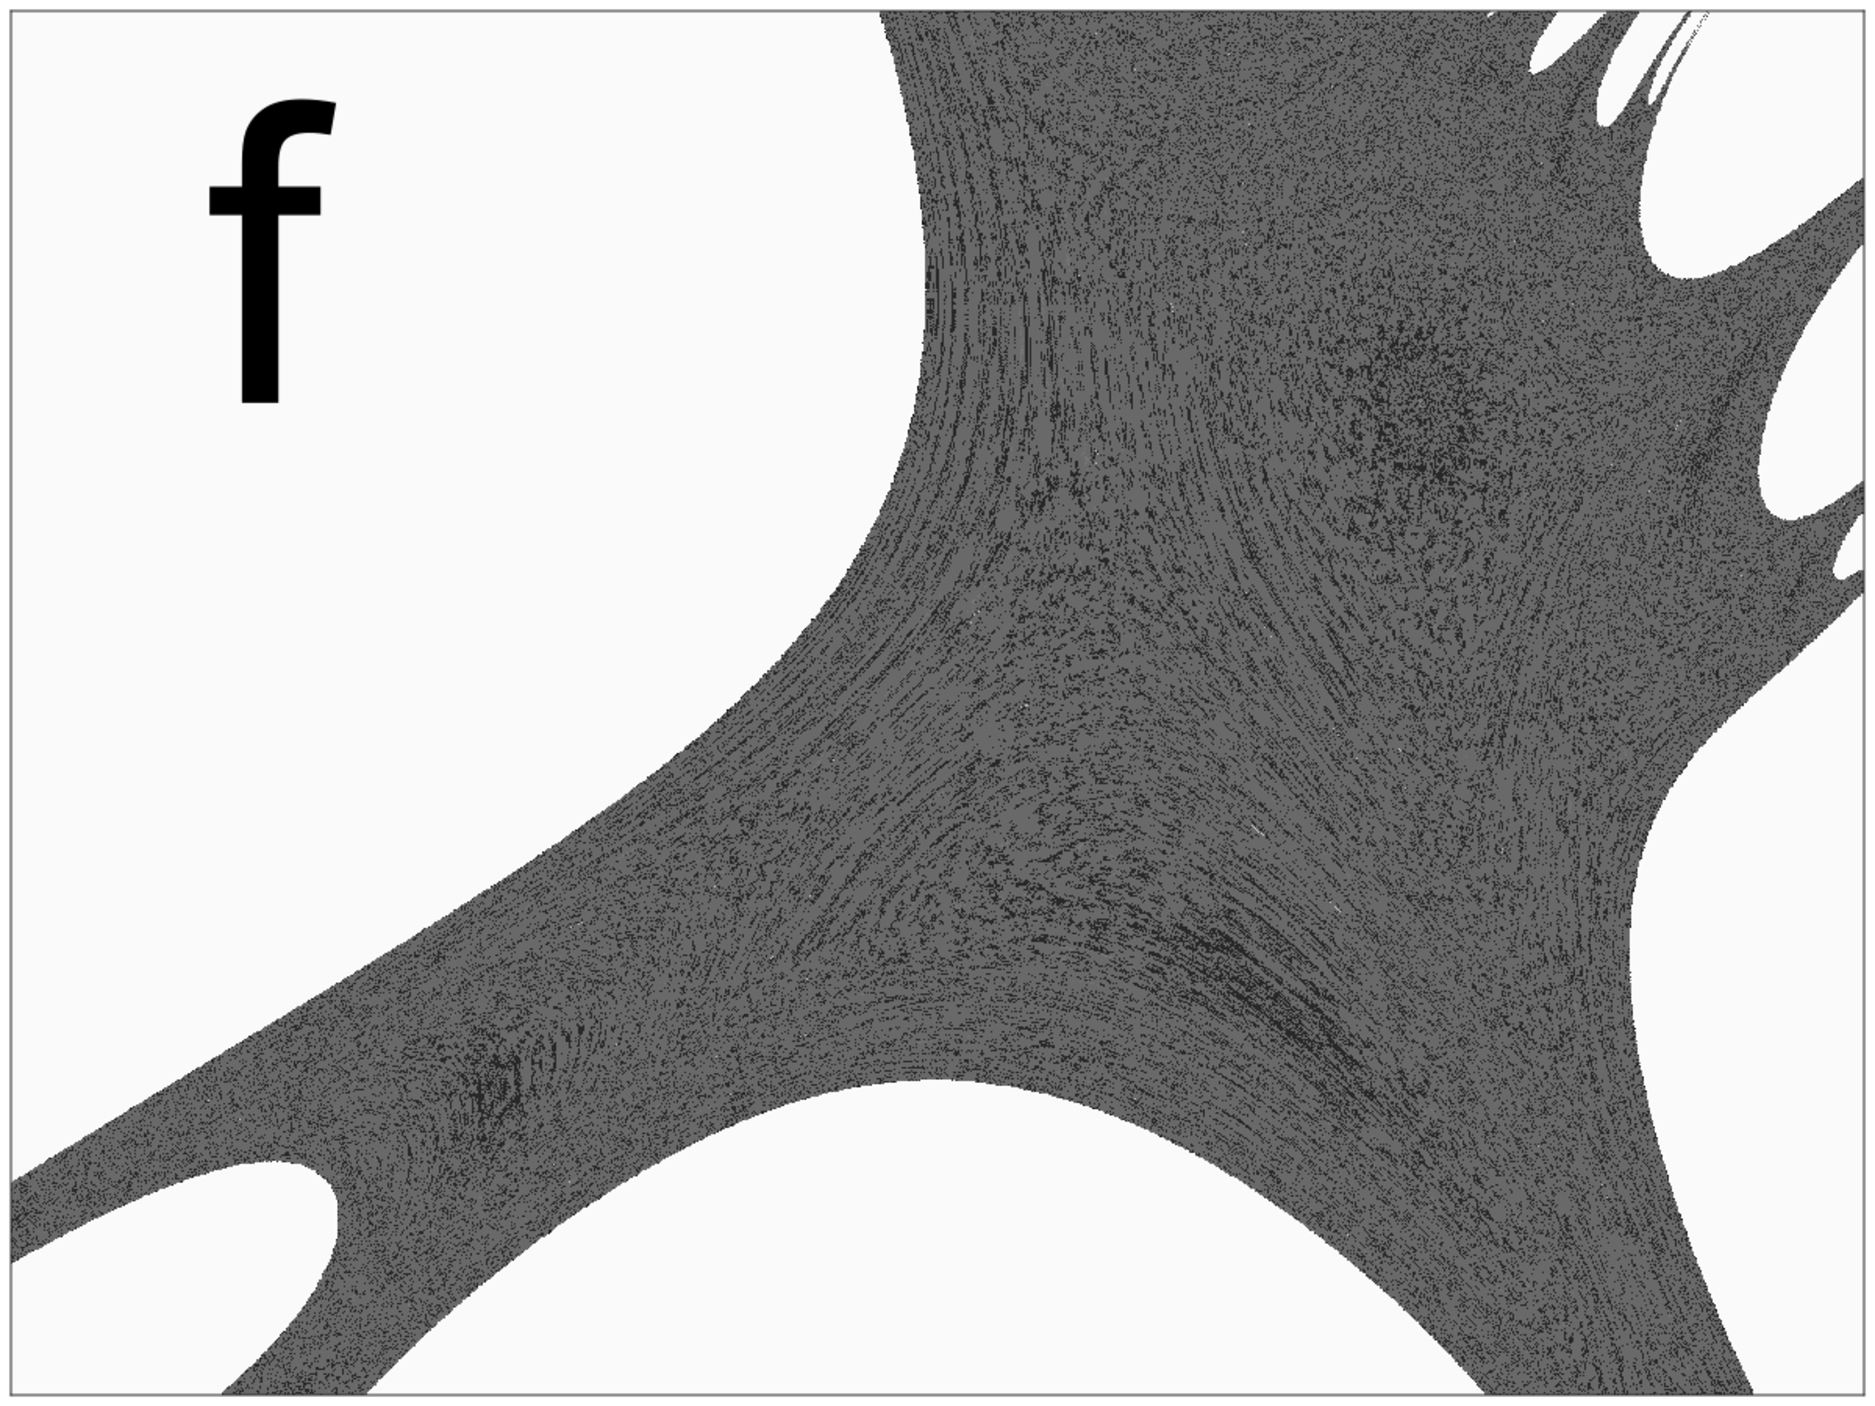
\includegraphics[width=0.32\textwidth]{m10_lu}\\
		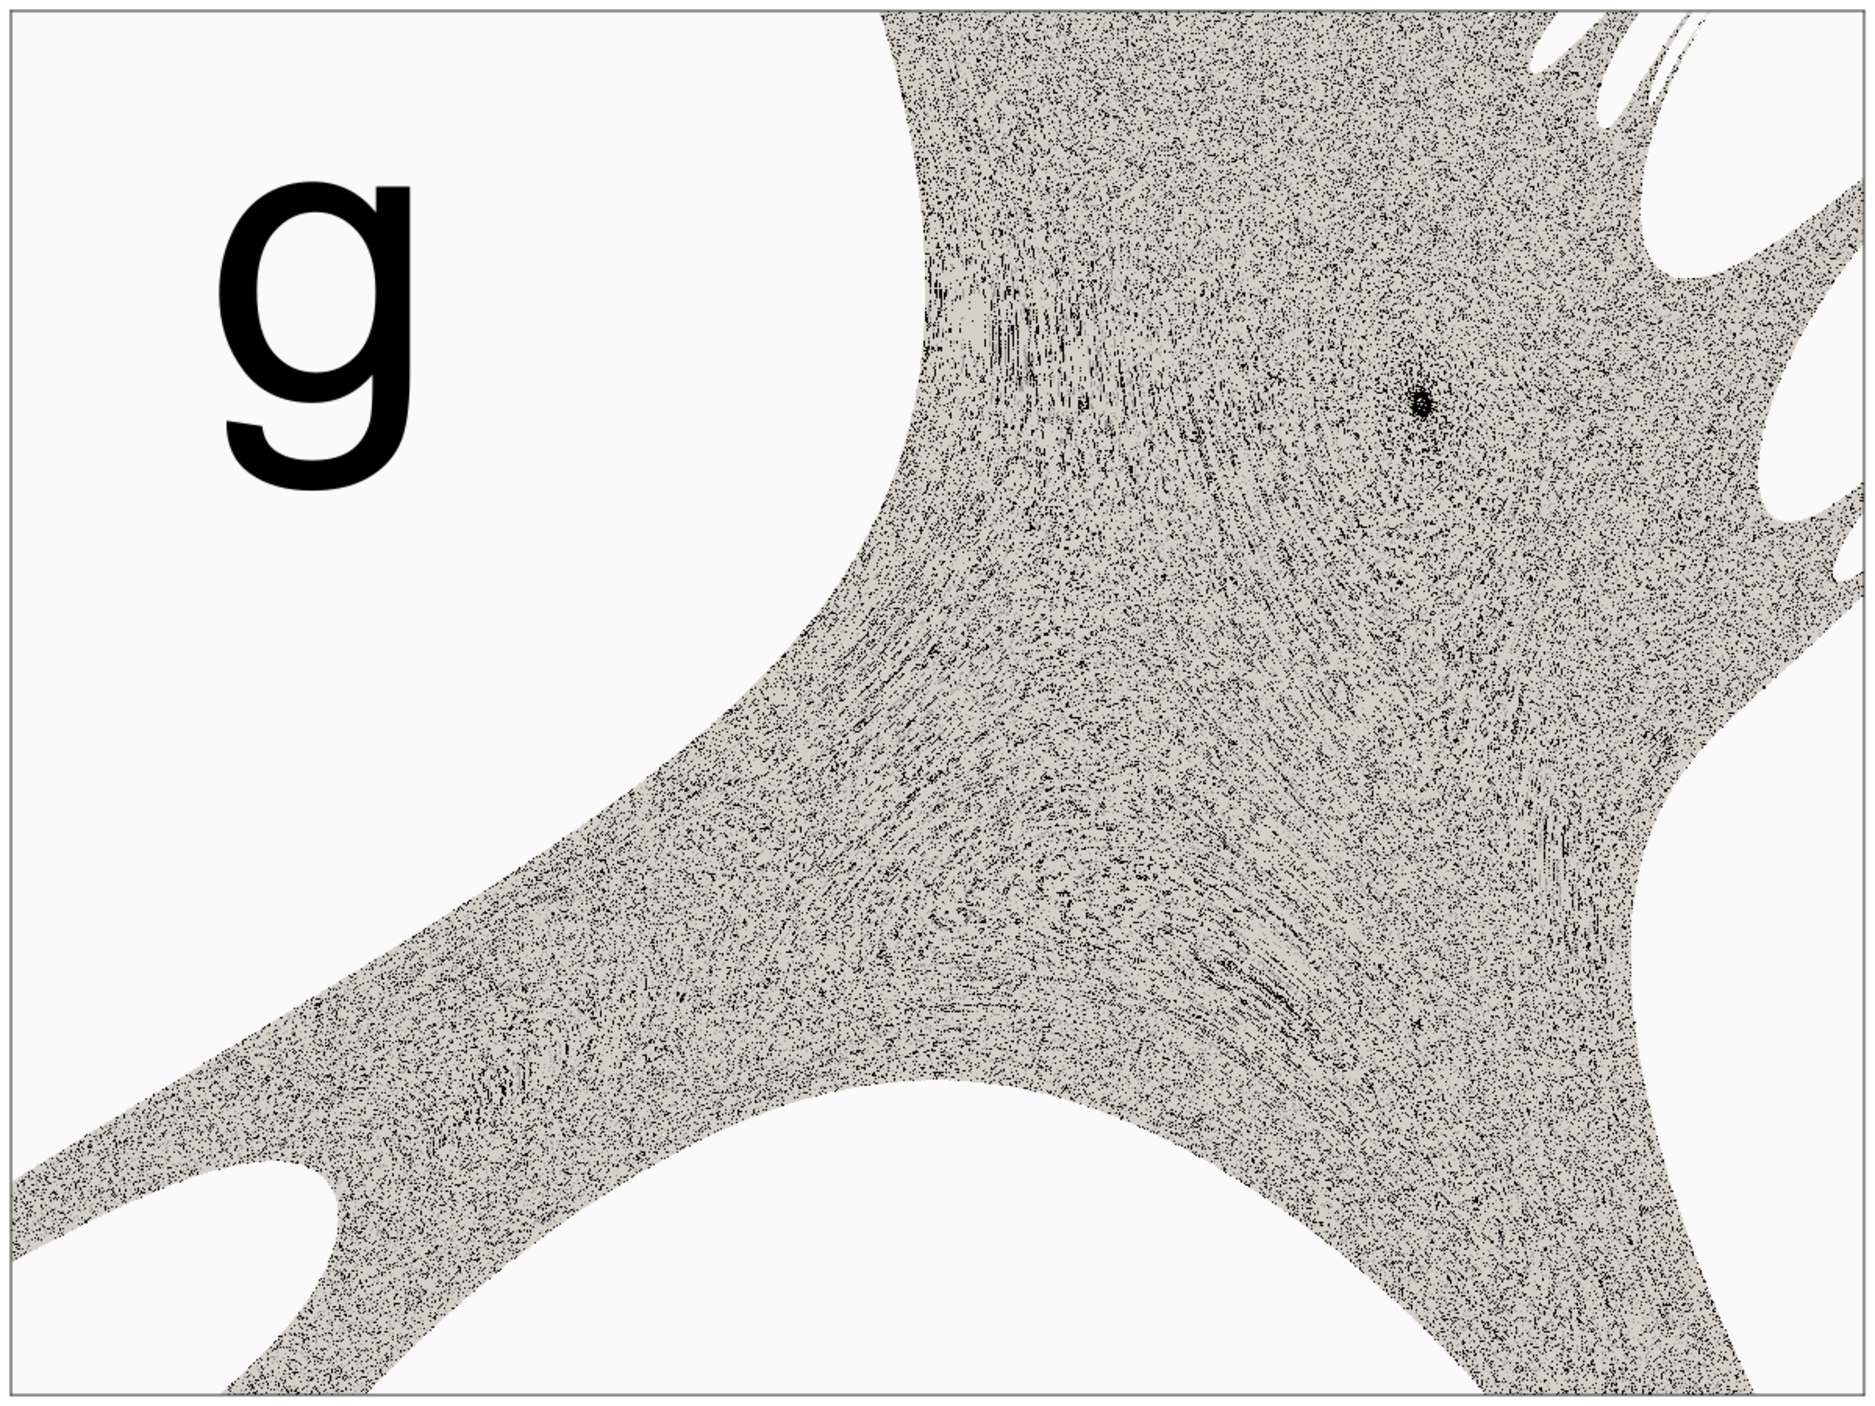
\includegraphics[width=0.32\textwidth]{m11_lu}
		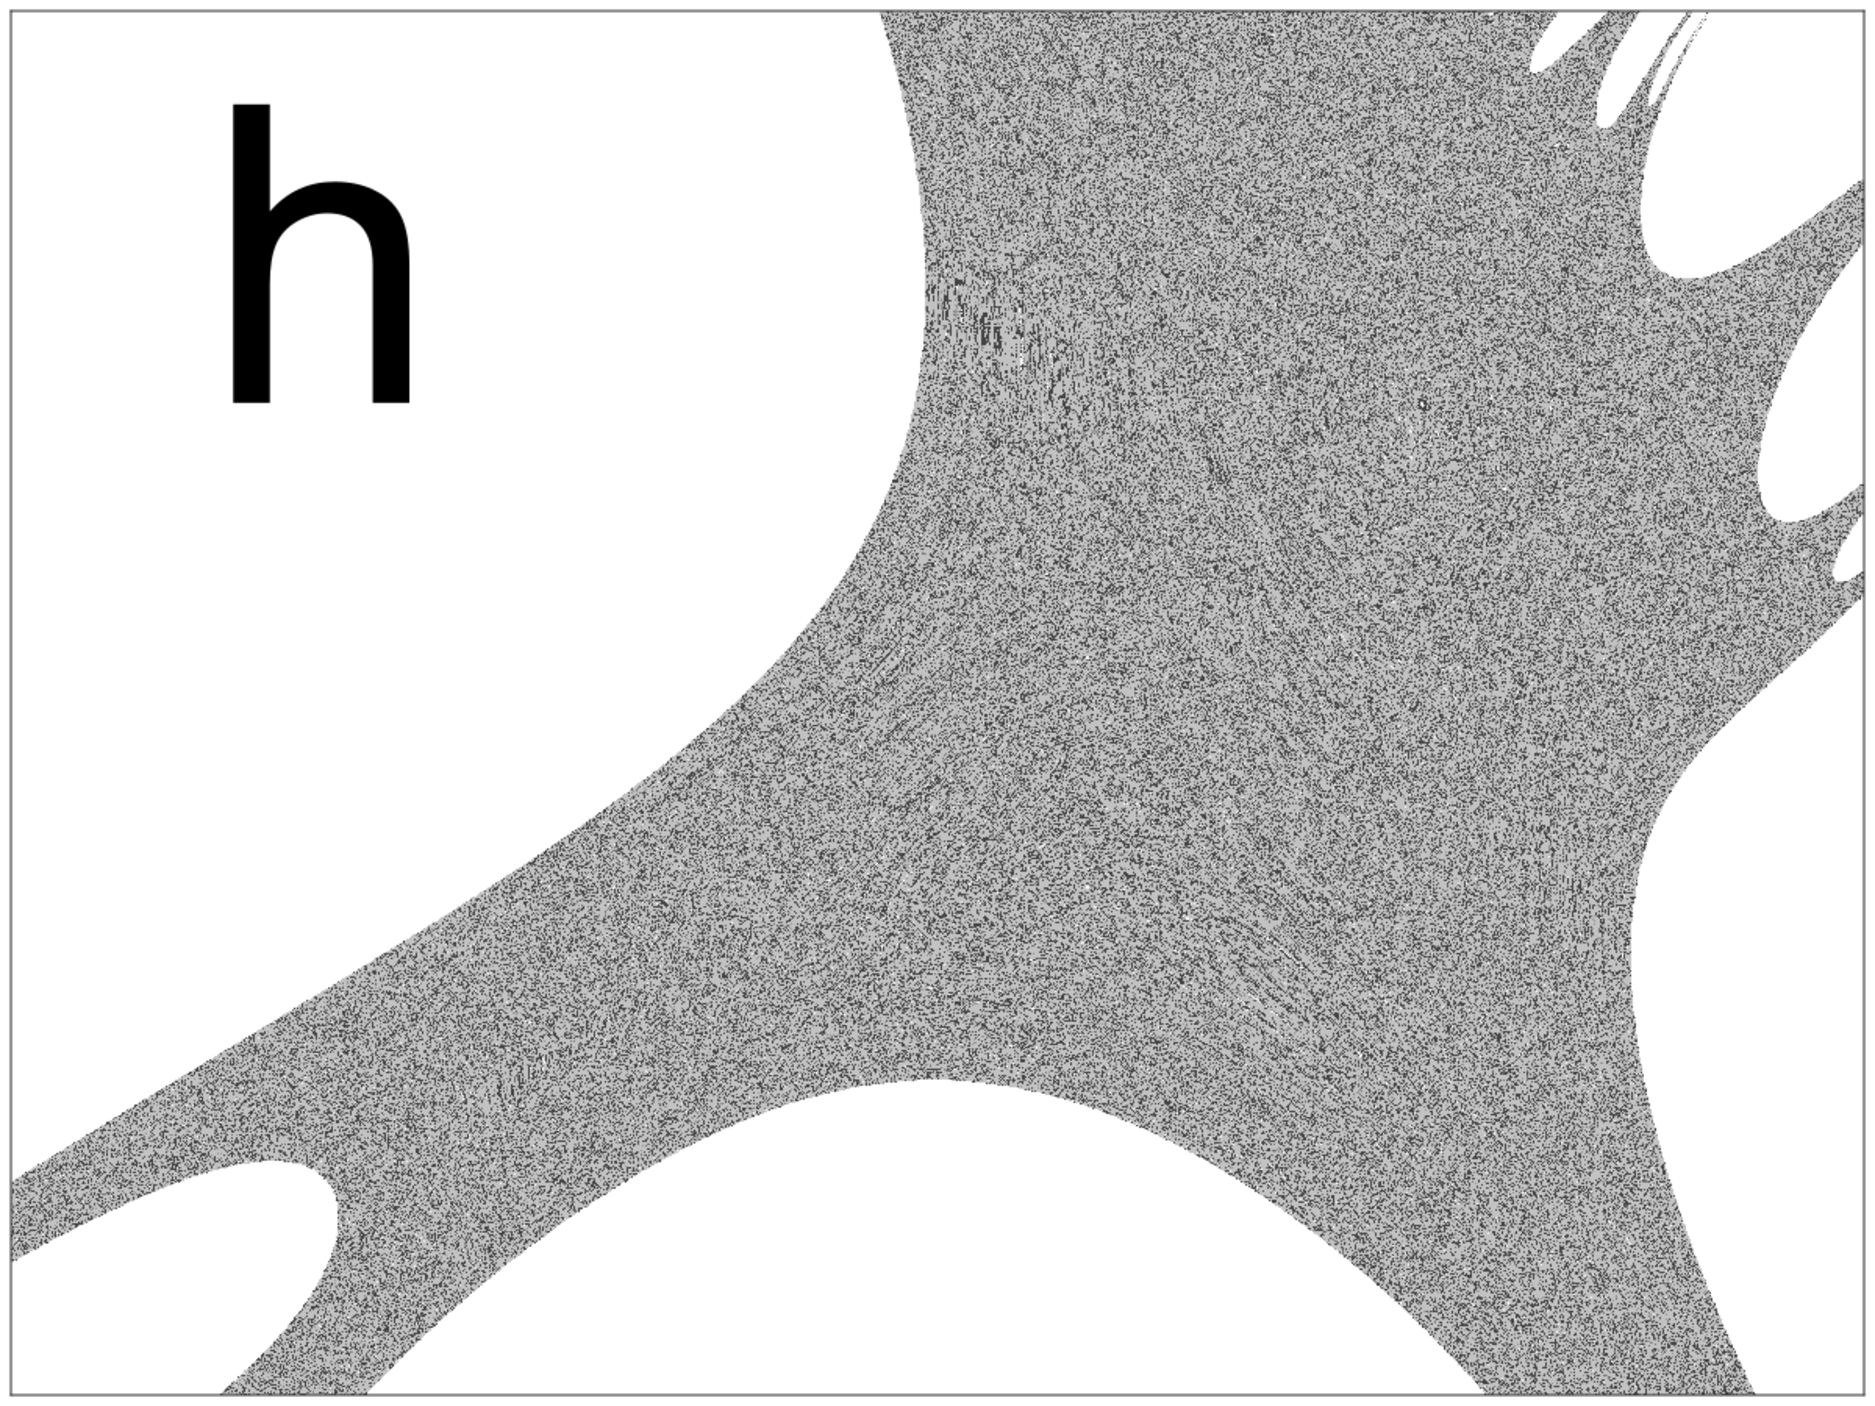
\includegraphics[width=0.32\textwidth]{m12_lu}
		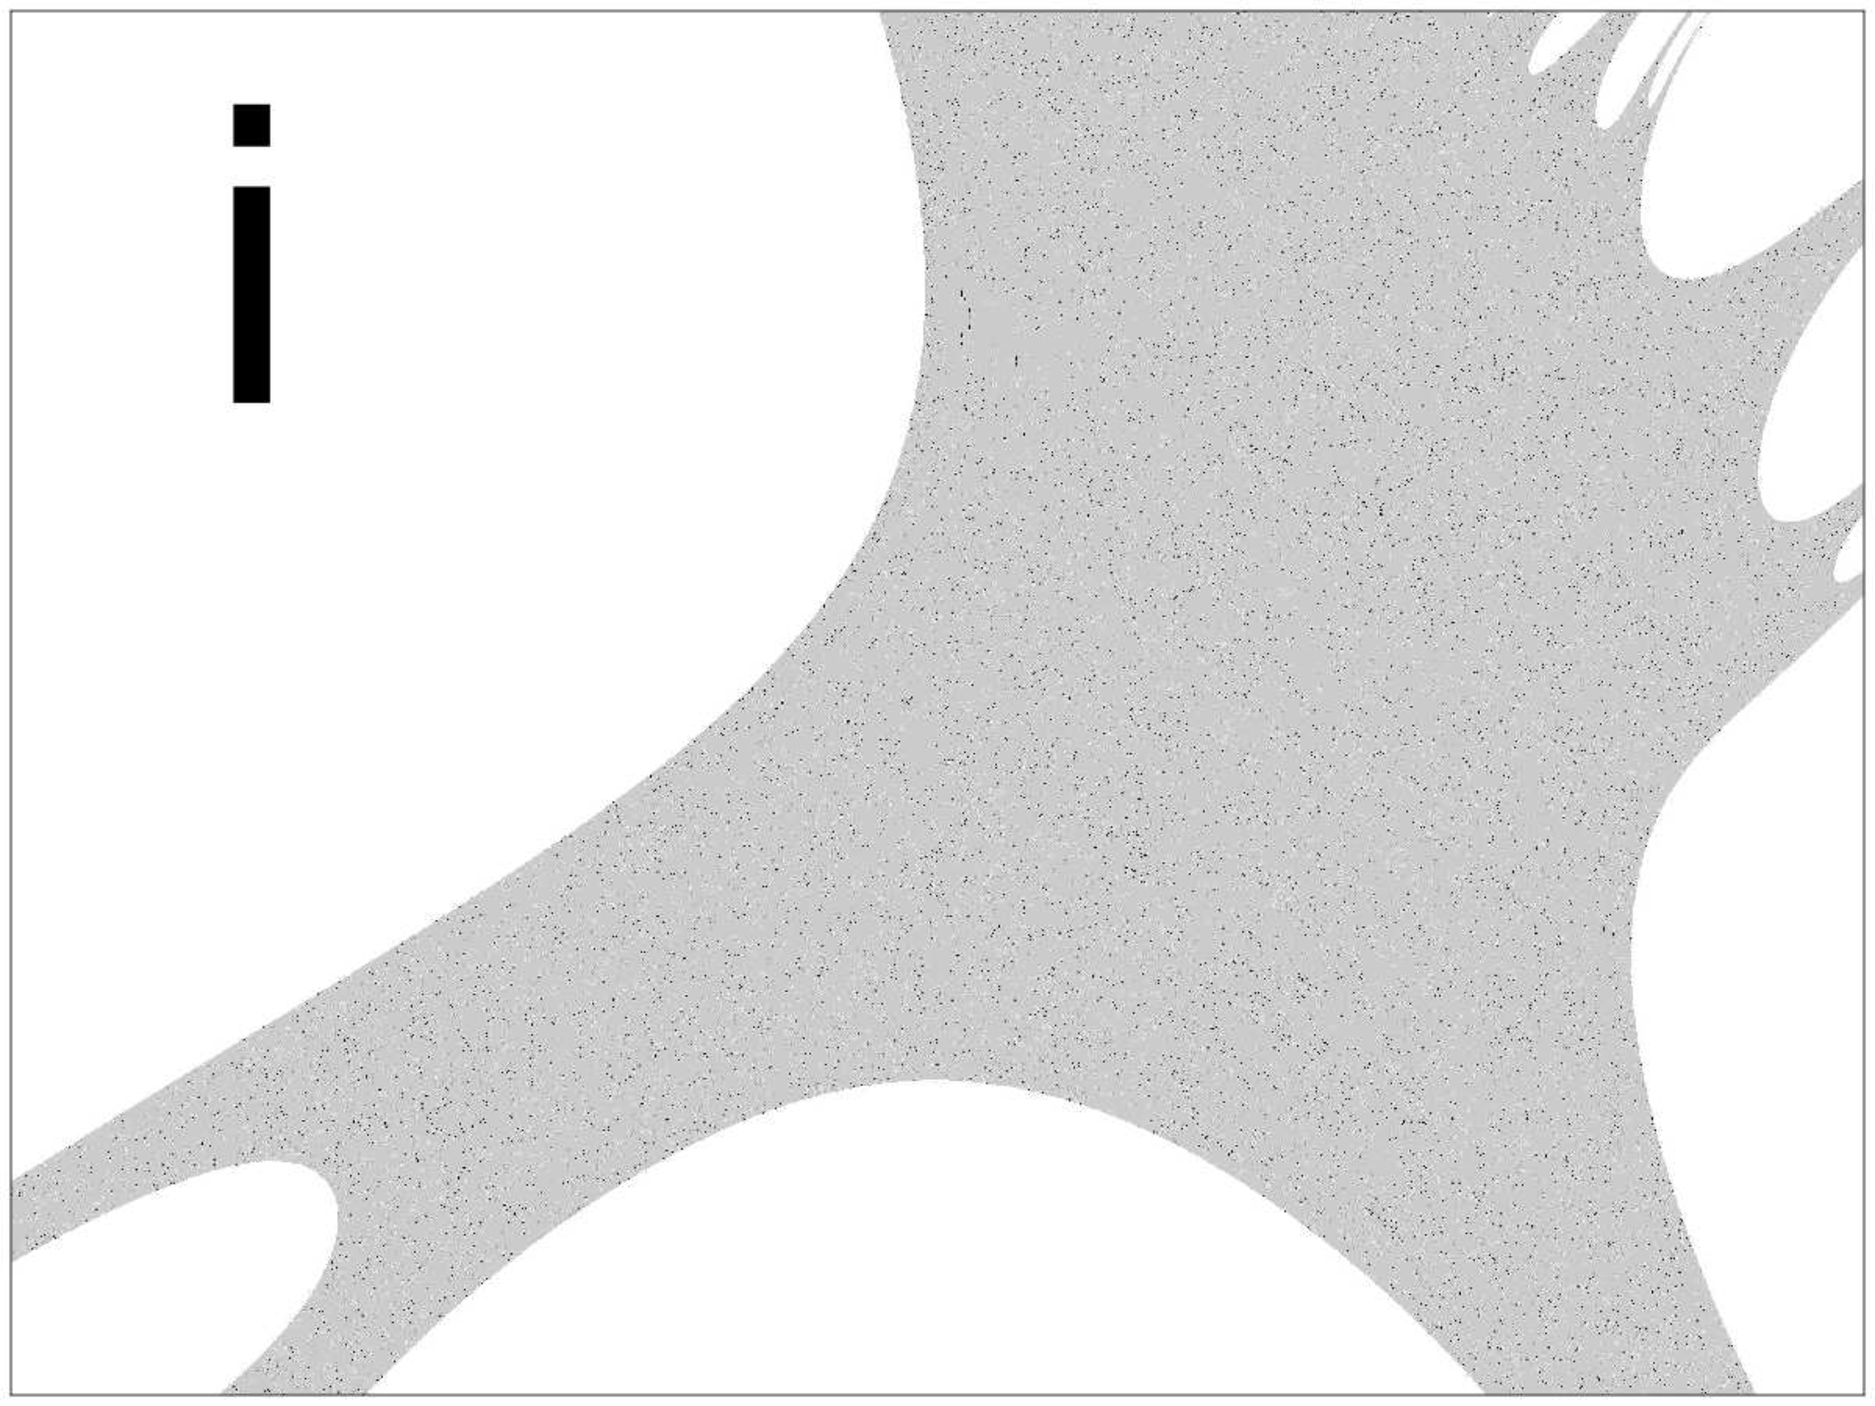
\includegraphics[width=0.32\textwidth]{m13_lu}\\
		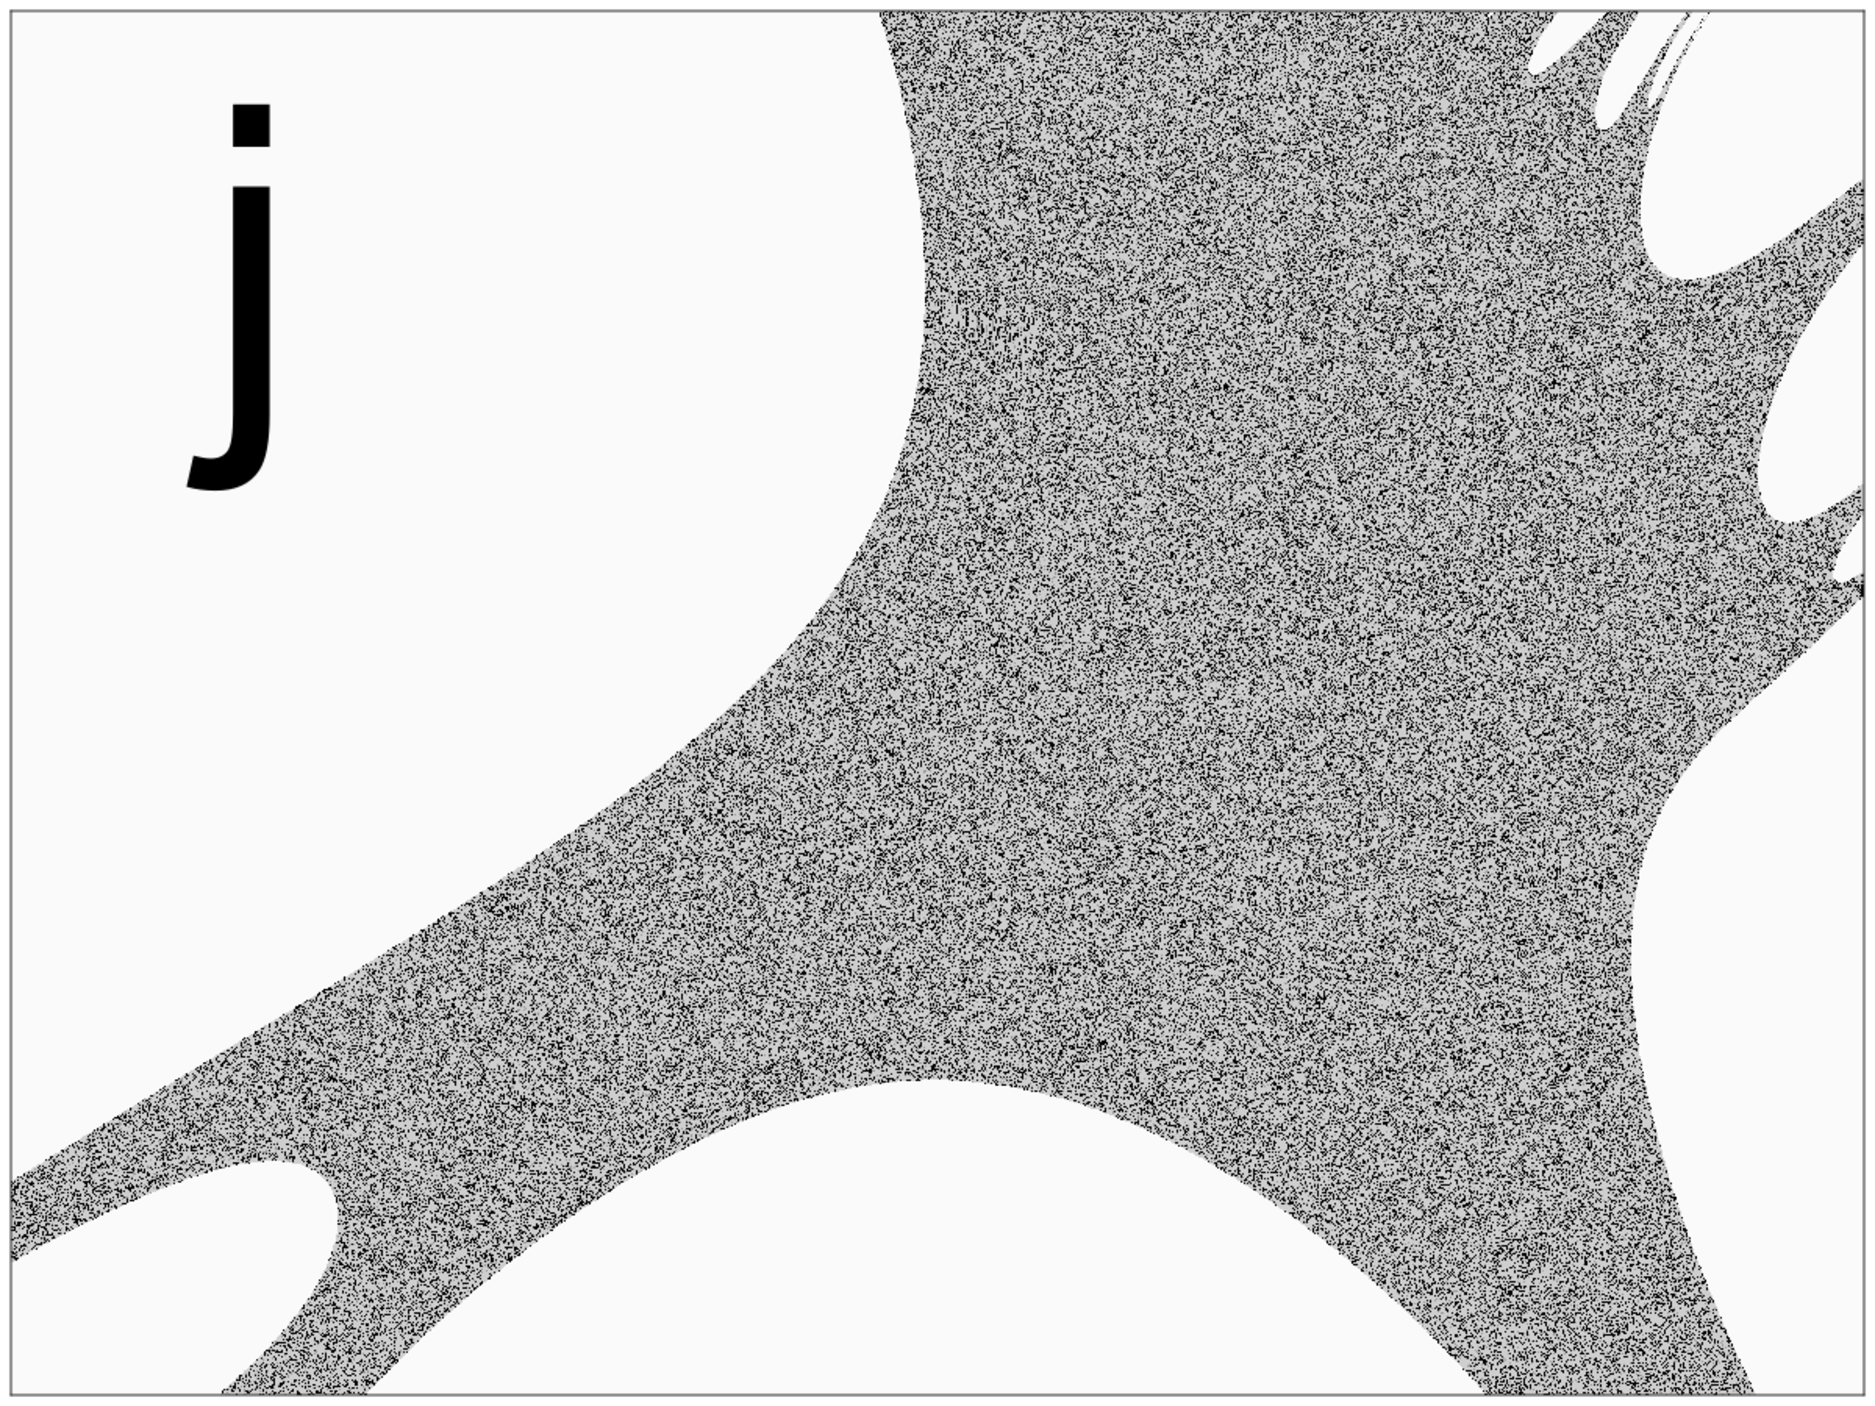
\includegraphics[width=0.32\textwidth]{m14_lu}
		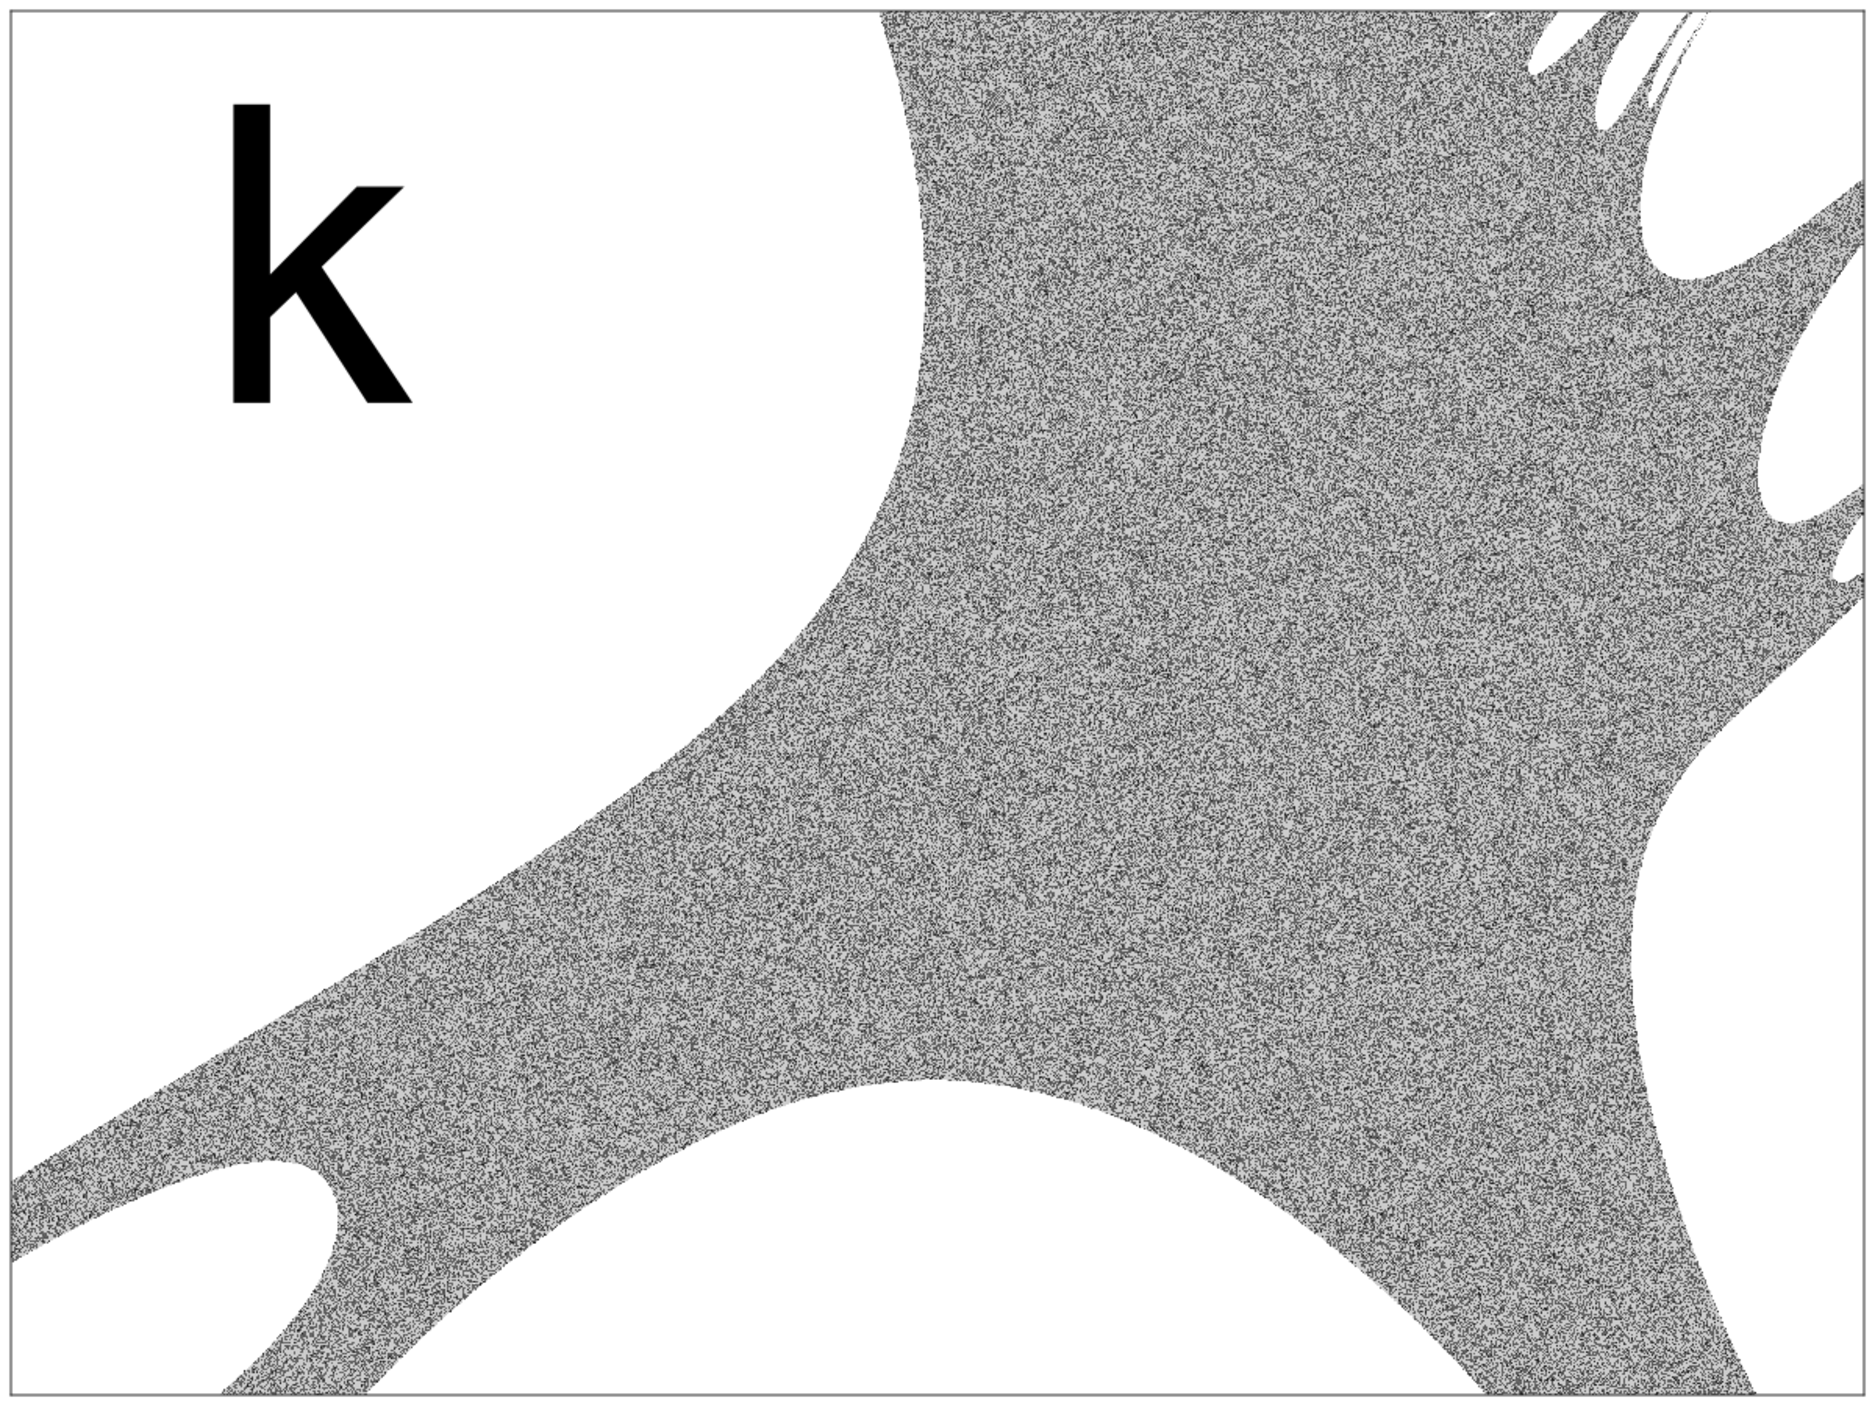
\includegraphics[width=0.32\textwidth]{m17_lu}
		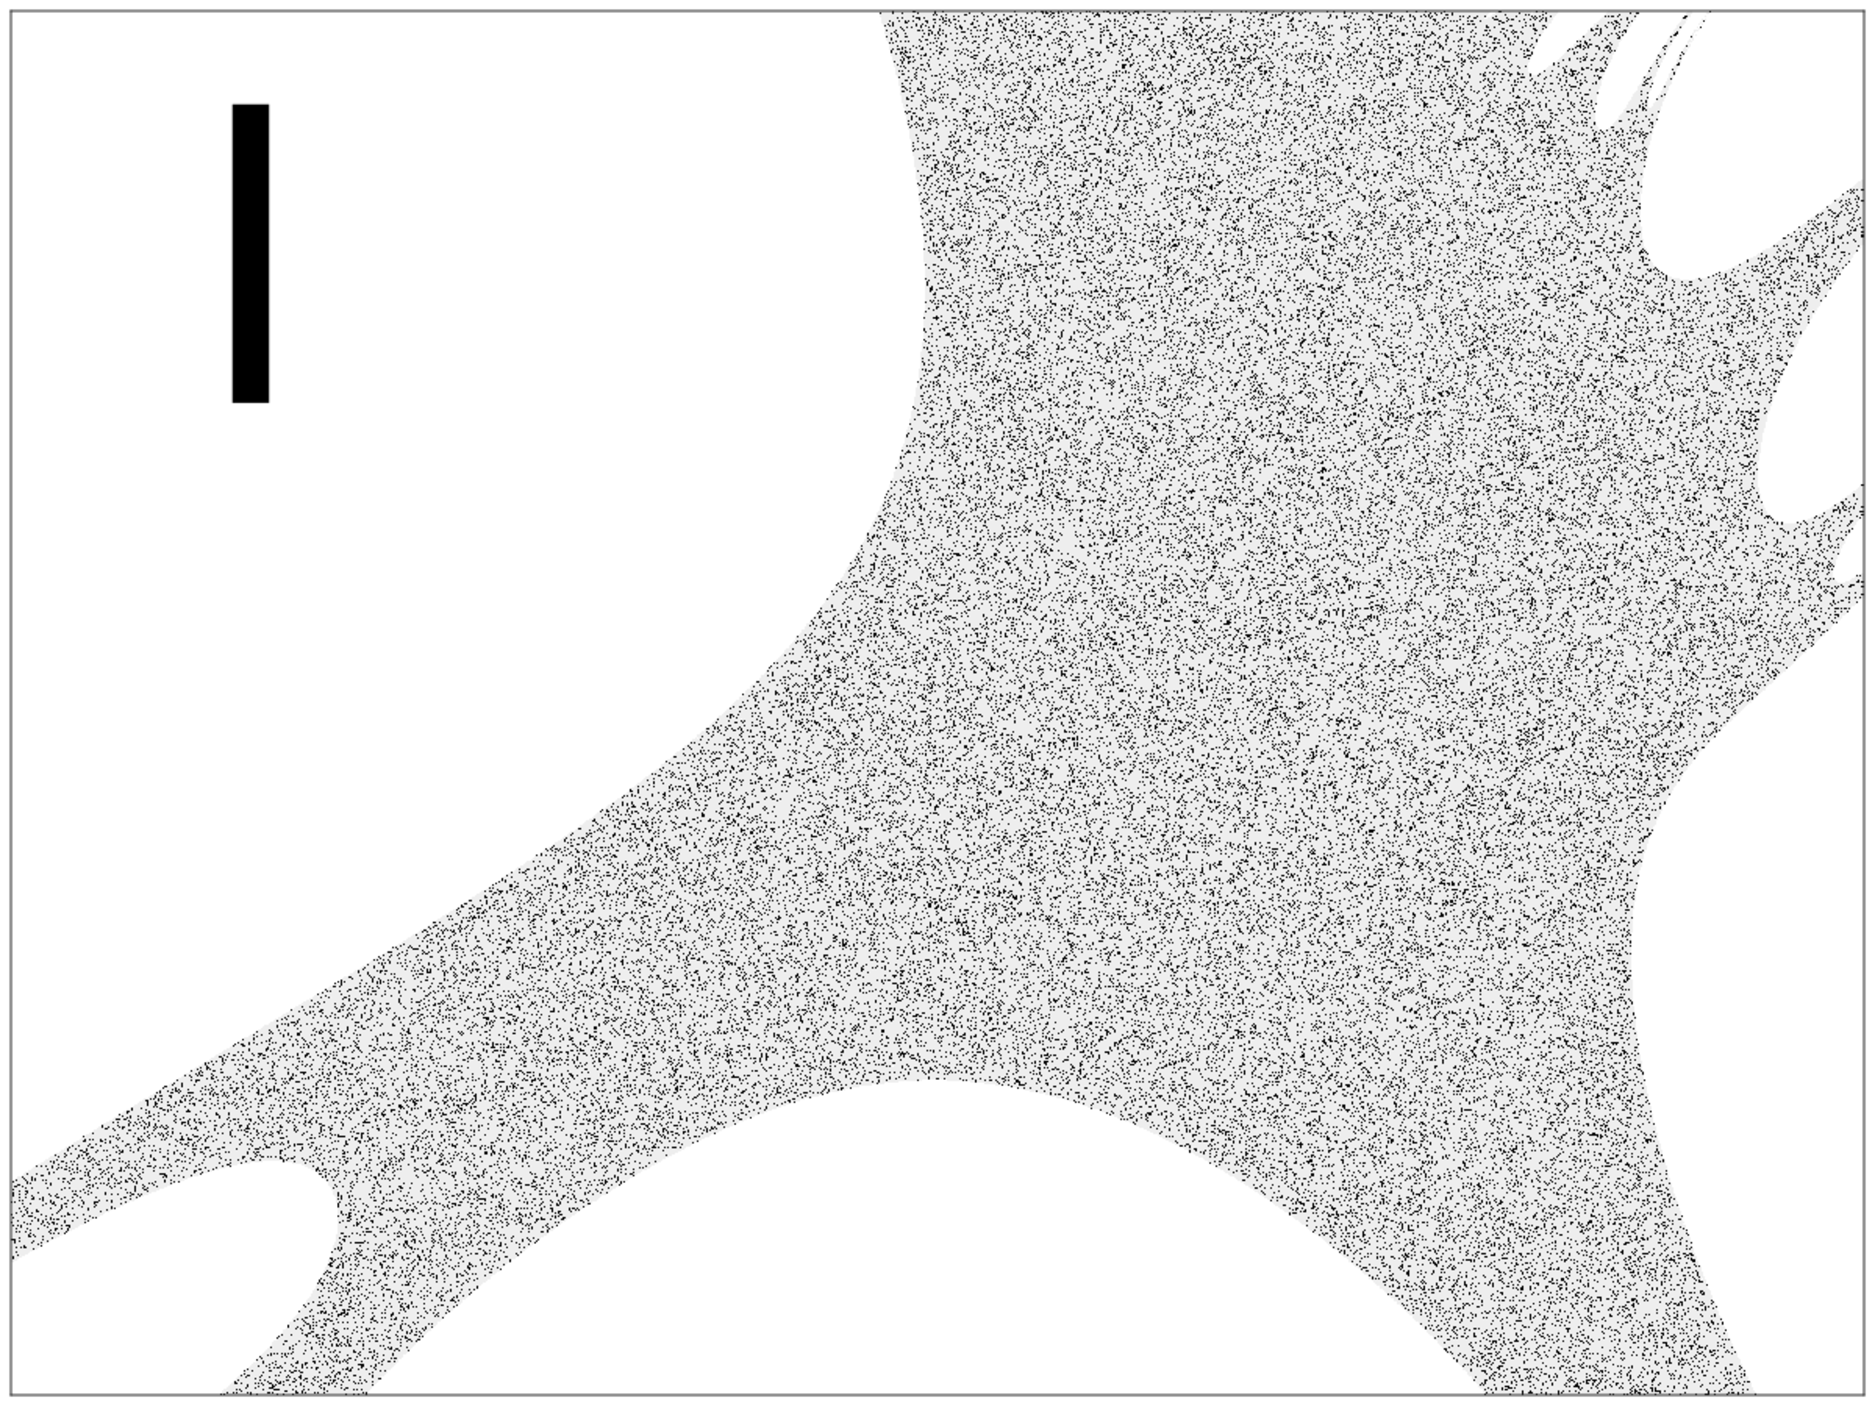
\includegraphics[width=0.32\textwidth]{m18_lu}\\
	\end{tabular}
	\caption{Áreas coexistentes en el dominio de atracción para: (a) $n_f=5$, (b) $n_f=6$, (c) $n_f=7$, (d) $n_f=8$, (e) $n_f=9$, (f) $n_f=10$, (g) $n_f=11$, (h) $n_f=12$, (i) $n_f=13$, (j) $n_f=14$, (k) $n_f=17$, (l) $n_f=18$.}
	\label{fig:avvelo}
\end{figure*}

Con el fin de poder distinguir las diferentes áreas coexistentes, se ha utilizado una amplia gama de tonos grises en cada Figura.
Se debe tener en cuenta que cada figura tiene su propio rango de grises, esto significa que, por ejemplo, un área casi blanca cuando $n_f = 5$ (Figura \ref{fig:avvelo} .a) corresponde a un período de $6$, mientras que un área más oscura en una Figura con mayor $n_f$ puede corresponder a un período superior a mil (Figura \ref{fig:avvelo} .e).
Estas cifras permiten reflejar los complejos dominios de atracción que aparecen al digitalizar.

Se puede ver en la Figura \ref{fig:avvelo} cuanto menor es el valor de $n_f$, mayor es el área de ICs que tiende a diverger y/o converger a puntos fijos.
A medida que $n_f$ aumenta, el área de puntos divergentes y fijos disminuye.
Estas Figuras junto con el Cuadro \ref{tabla} permiten interpretar fácilmente el comportamiento del sistema.
En el Cuadro \ref{tabla} las longitudes de las secuencias que aparecen en el dominio de atracción para cada $n_f$ se ordenan por el número de circuitos integrados menos numerosos que convergen en ese ciclo.
Además, entre paréntesis se presenta la tasa de ocurrencia.
De hecho, las Figuras con valores más bajos de $n_f$ presentan superficies irregulares o rugosas, señalando que los ciclos de diferentes longitudes coexisten.
Por ejemplo, para $n_f = 5$ hay una prevalencia de ciclos de períodos cortos.
En ese caso, existen solo dos ciclos límite, la zona gris más clara corresponde al dominio de atracción de los ciclos límite de longitud seis, que es el ciclo menos numeroso, de acuerdo con el Cuadro \ref{tabla}, y la zona más oscura corresponde al dominio de atracción de longitud de ciclo dos.

Aunque para $n_f \geqslant 13$ (Figuras \ref{fig:avvelo}.i a \ref{fig:avvelo}.l), el dominio de atracción parece ser suave y uniforme, todavía hay ciclos con diferentes períodos que coexisten en el atractor por $ n_f = 14 $, $ 17 $ y $ 18 $.
Esto se puede ver si ampliamos una Sección de las figuras (Figura \ref{fig:m_zoom}).
%
\begin{figure}
	\centering
	\begin{subfigure}[t]{0.49\textwidth}
		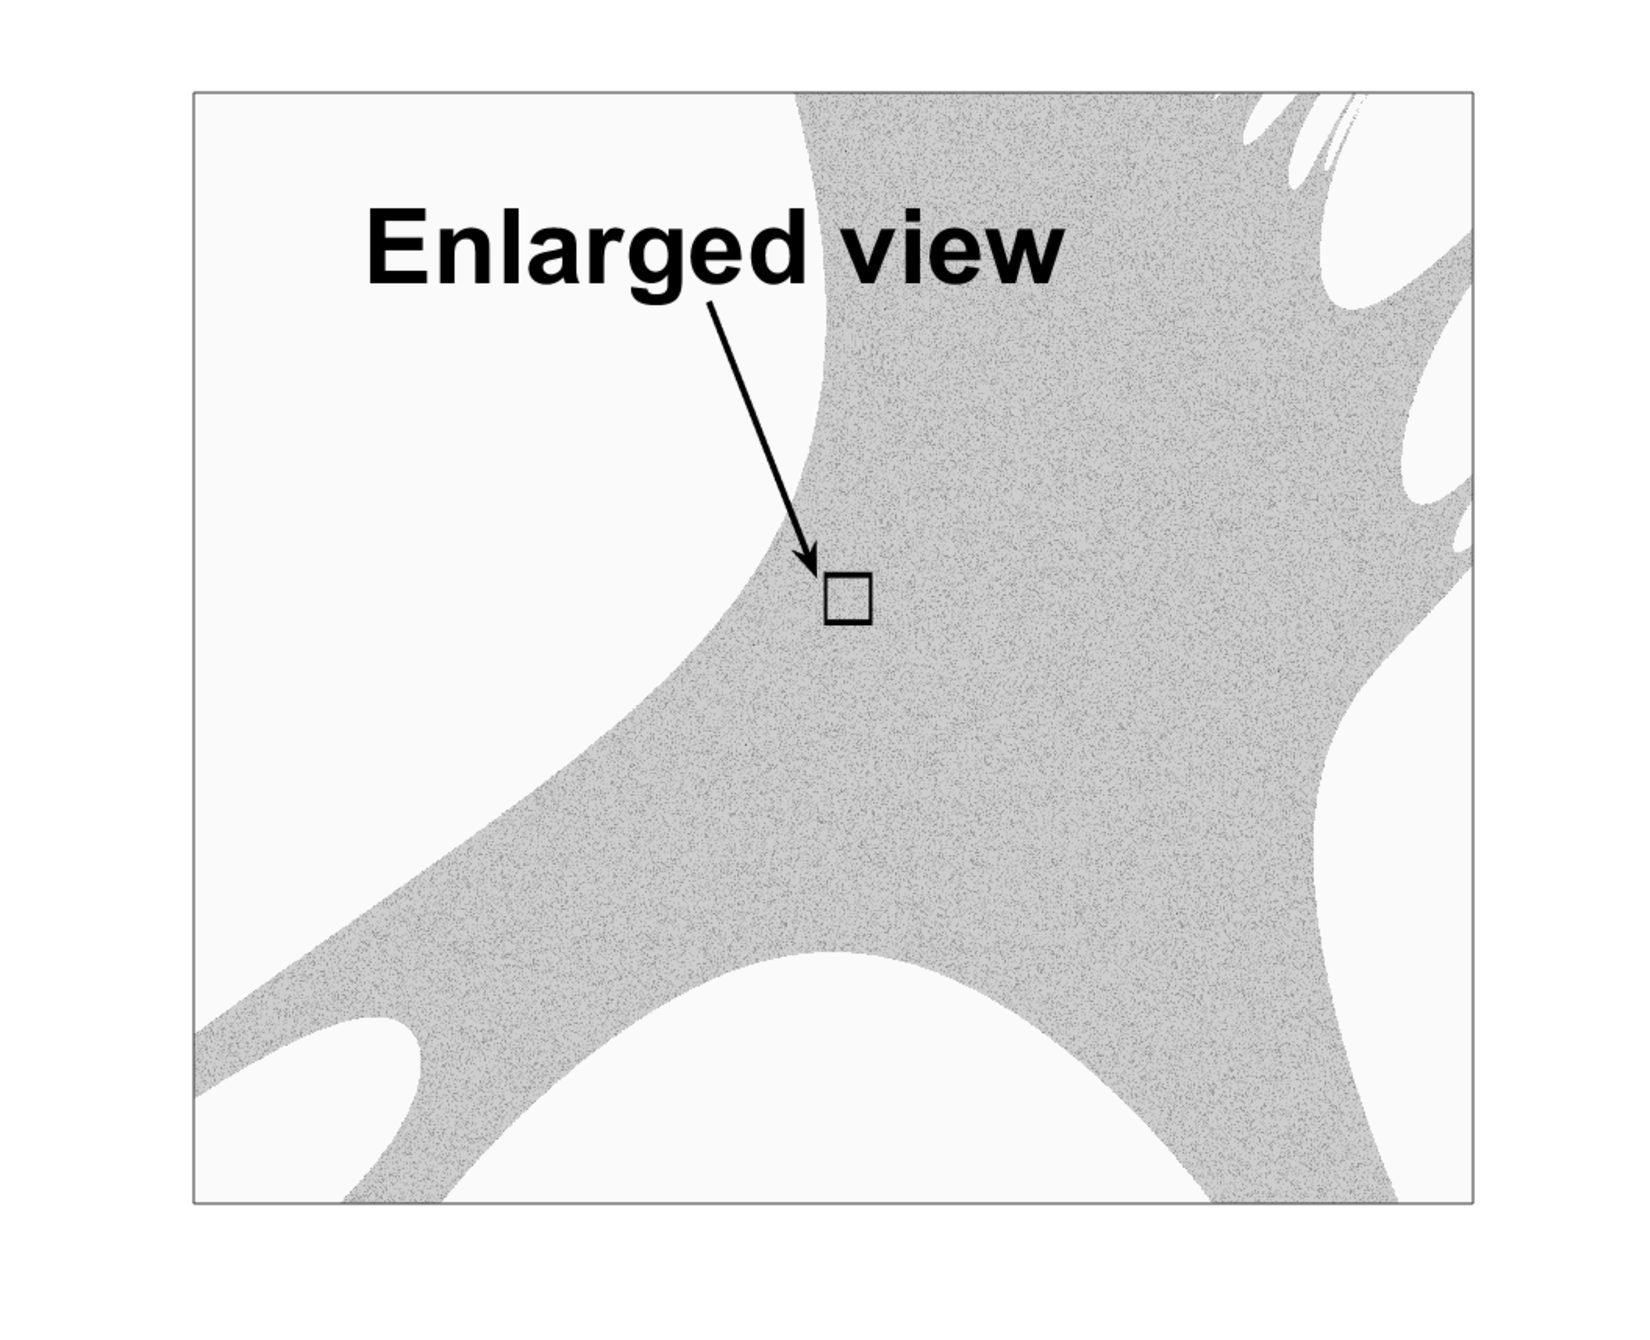
\includegraphics[width=\textwidth]{m_zoom}
		\caption{Sección rectangular del dominio de atracción, sección $[0.3\pm 0.001, -0.2\pm 0.001]$.}
		\label{fig:gull}
	\end{subfigure}
	\hfill 
	\begin{subfigure}[t]{0.49\textwidth}
		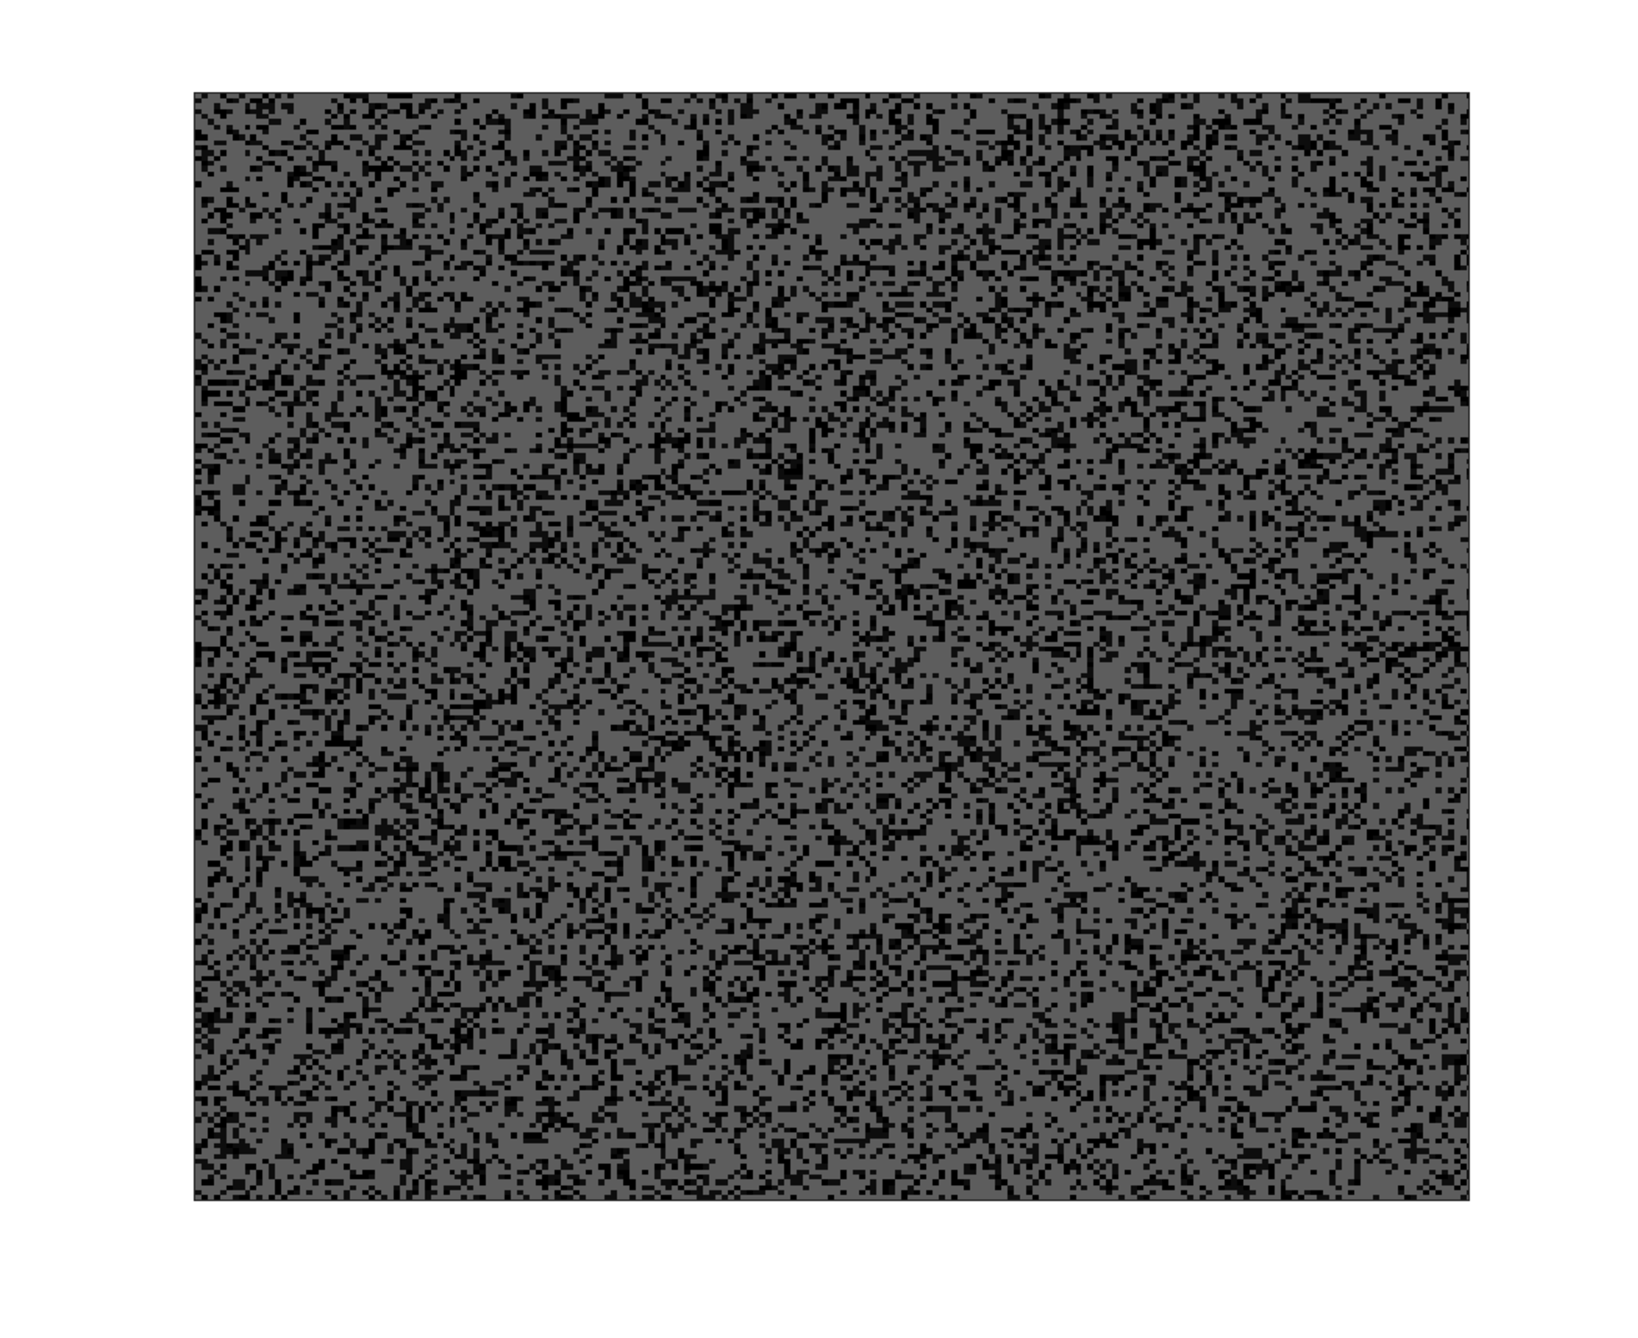
\includegraphics[width=\textwidth]{m14_lu_zoomO}
		\caption{$n_f=14$.}
		\label{fig:tiger}
	\end{subfigure}
	\hfill  
	\begin{subfigure}[t]{0.49\textwidth}
		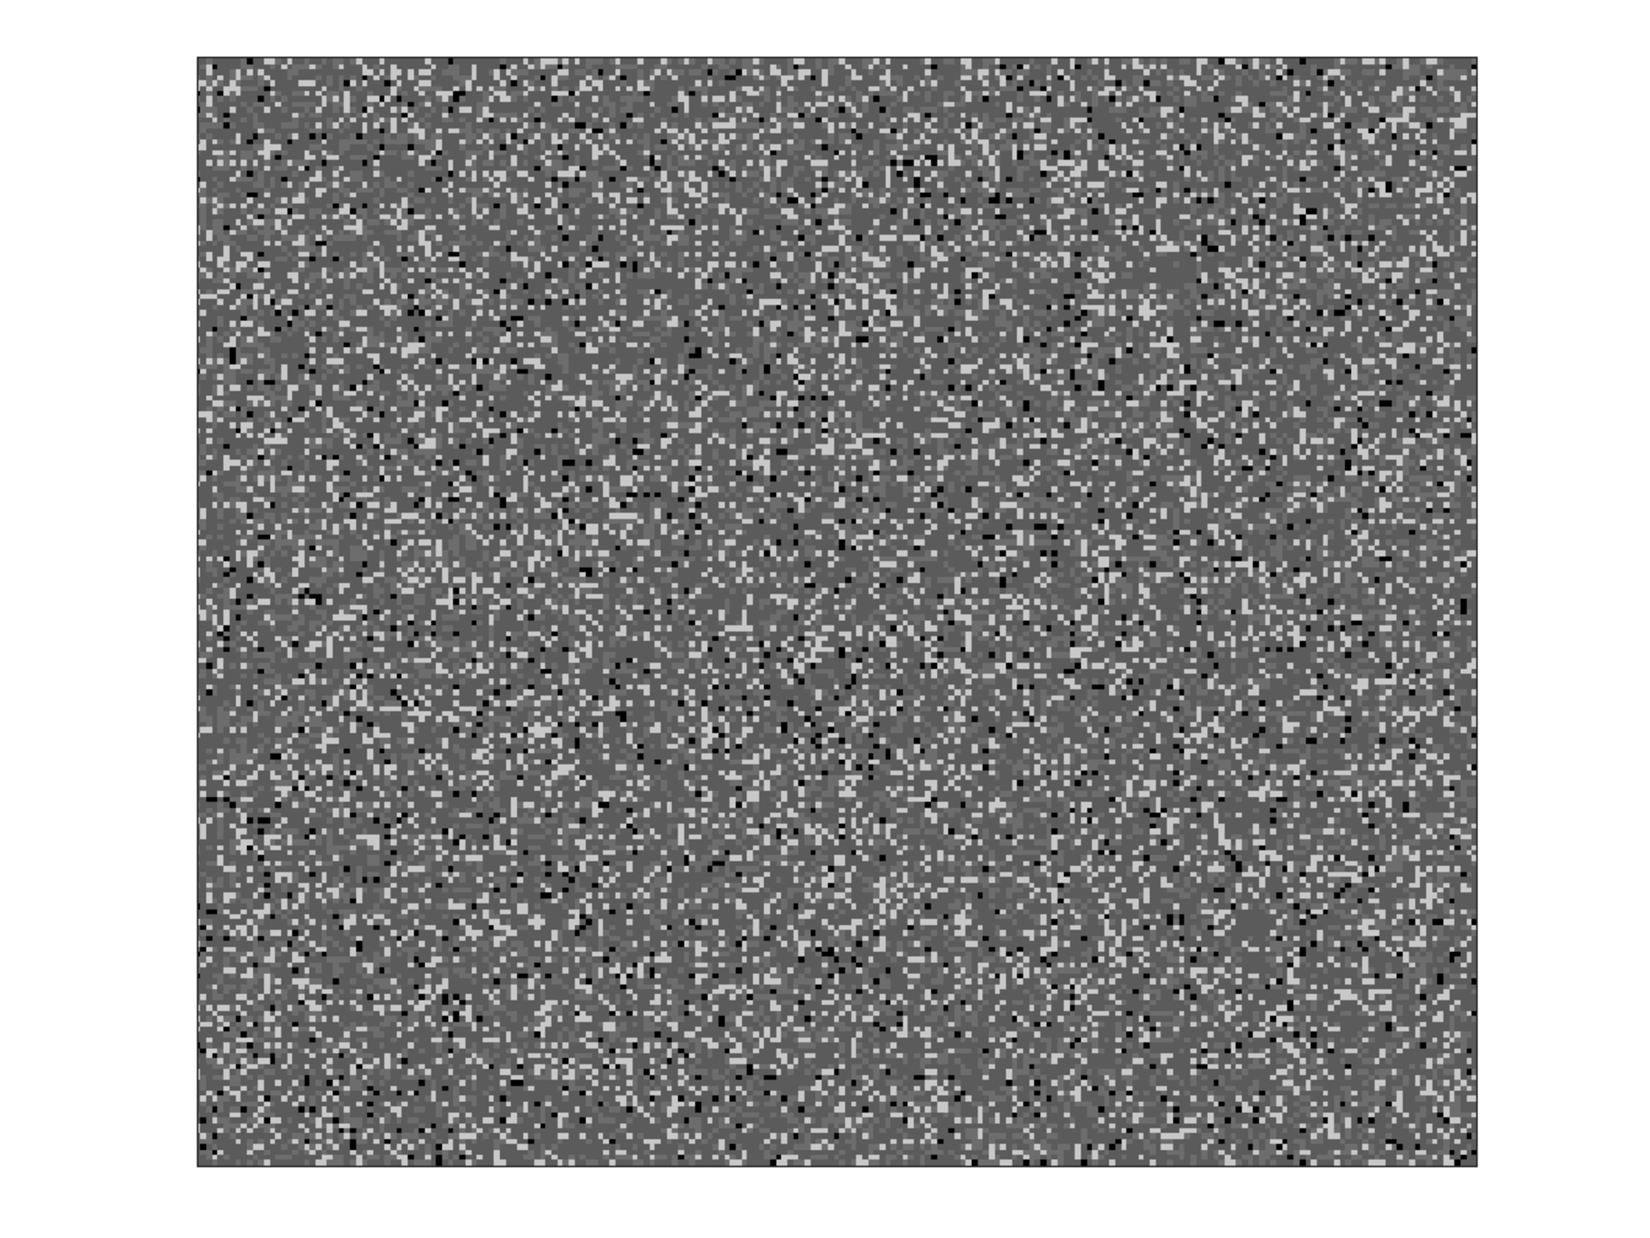
\includegraphics[width=\textwidth]{m17_lu_zoomO}
		\caption{$n_f=17$.}
		\label{fig:mouse}
	\end{subfigure}
	\hfill   
	\begin{subfigure}[t]{0.49\textwidth}
		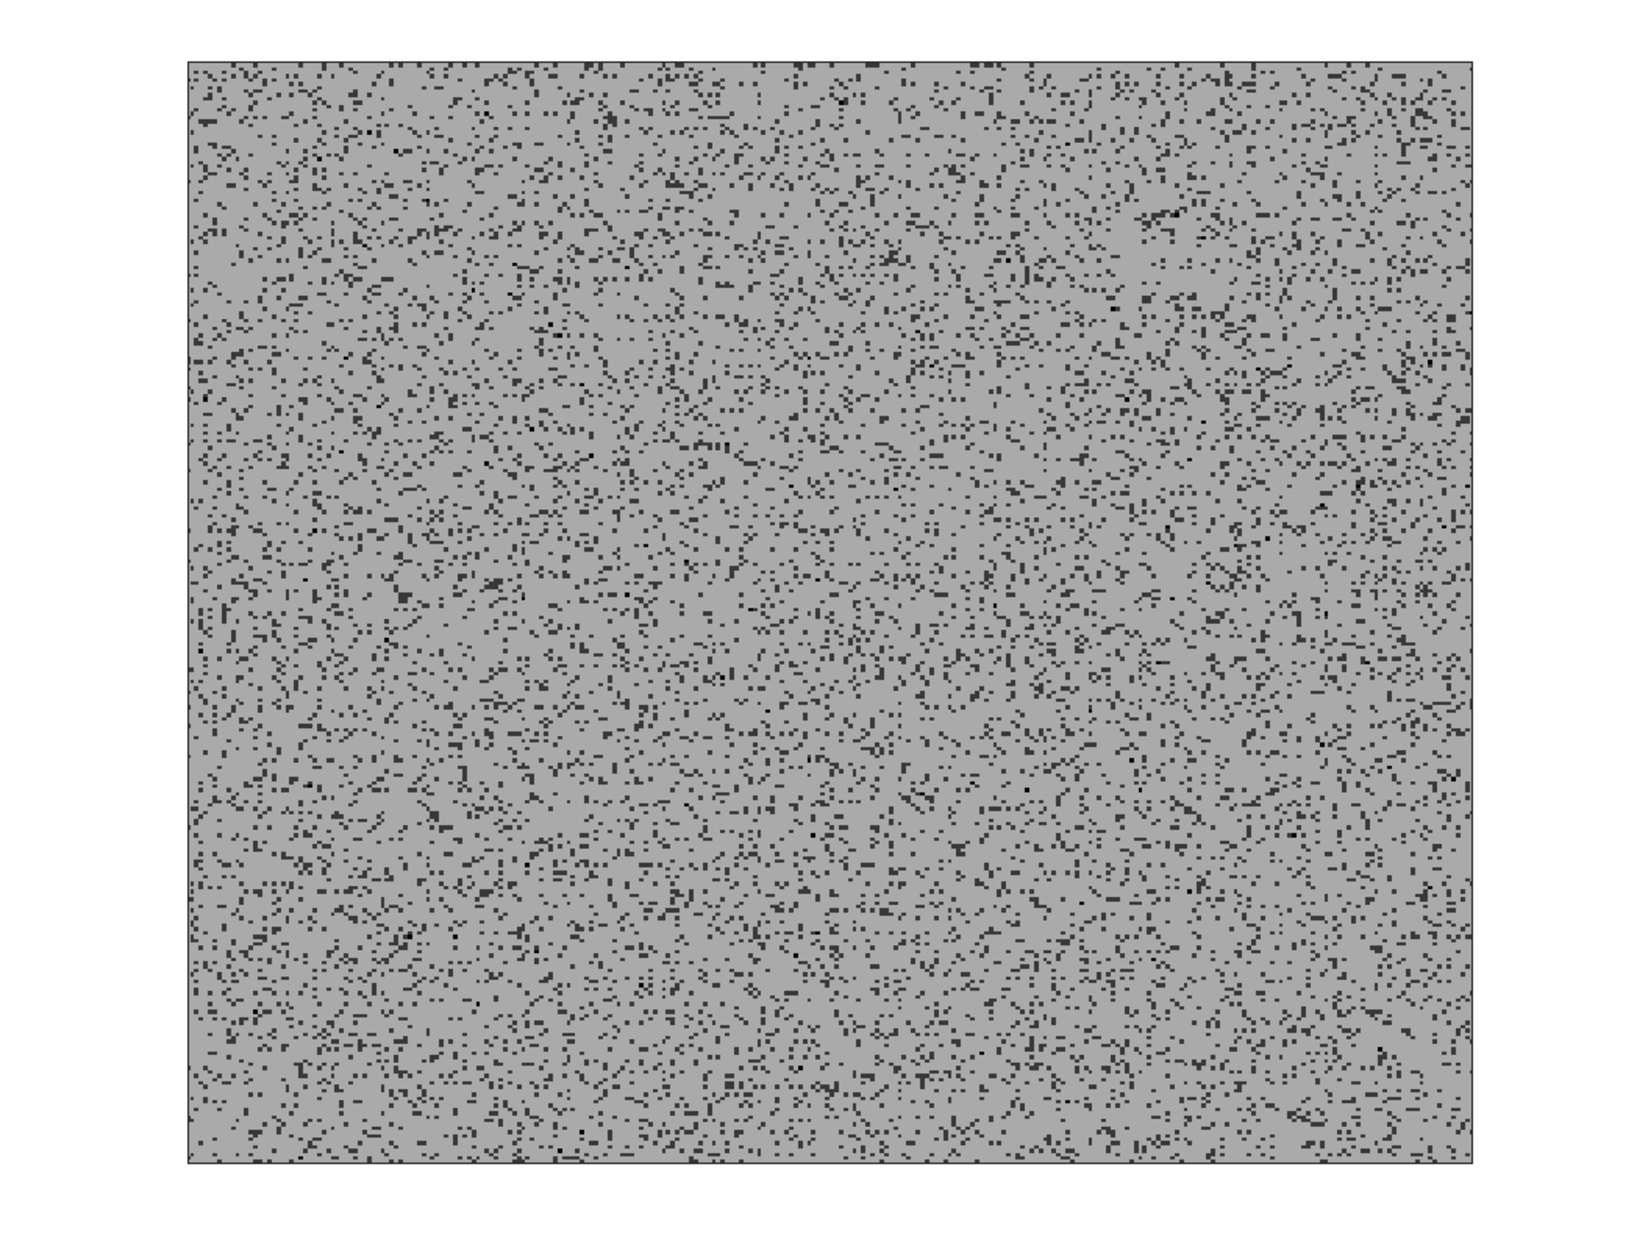
\includegraphics[width=\textwidth]{m18_lu_zoomO}
		\caption{$n_f=18$.}
		\label{fig:mouse}
	\end{subfigure}
	\caption{Vistas ampliadas del dominio de atracción para distintos valores de $n_f$.}\label{fig:m_zoom}
\end{figure}

Sin embargo, cuando queremos hacer una comparación general de lo que ocurre con los períodos cuando varían las precisiones, se requiere una escala de colores, ver Figura \ref{fig:m}.
%
\begin{figure*}
	\centering
	\begin{tabular}{cc}
		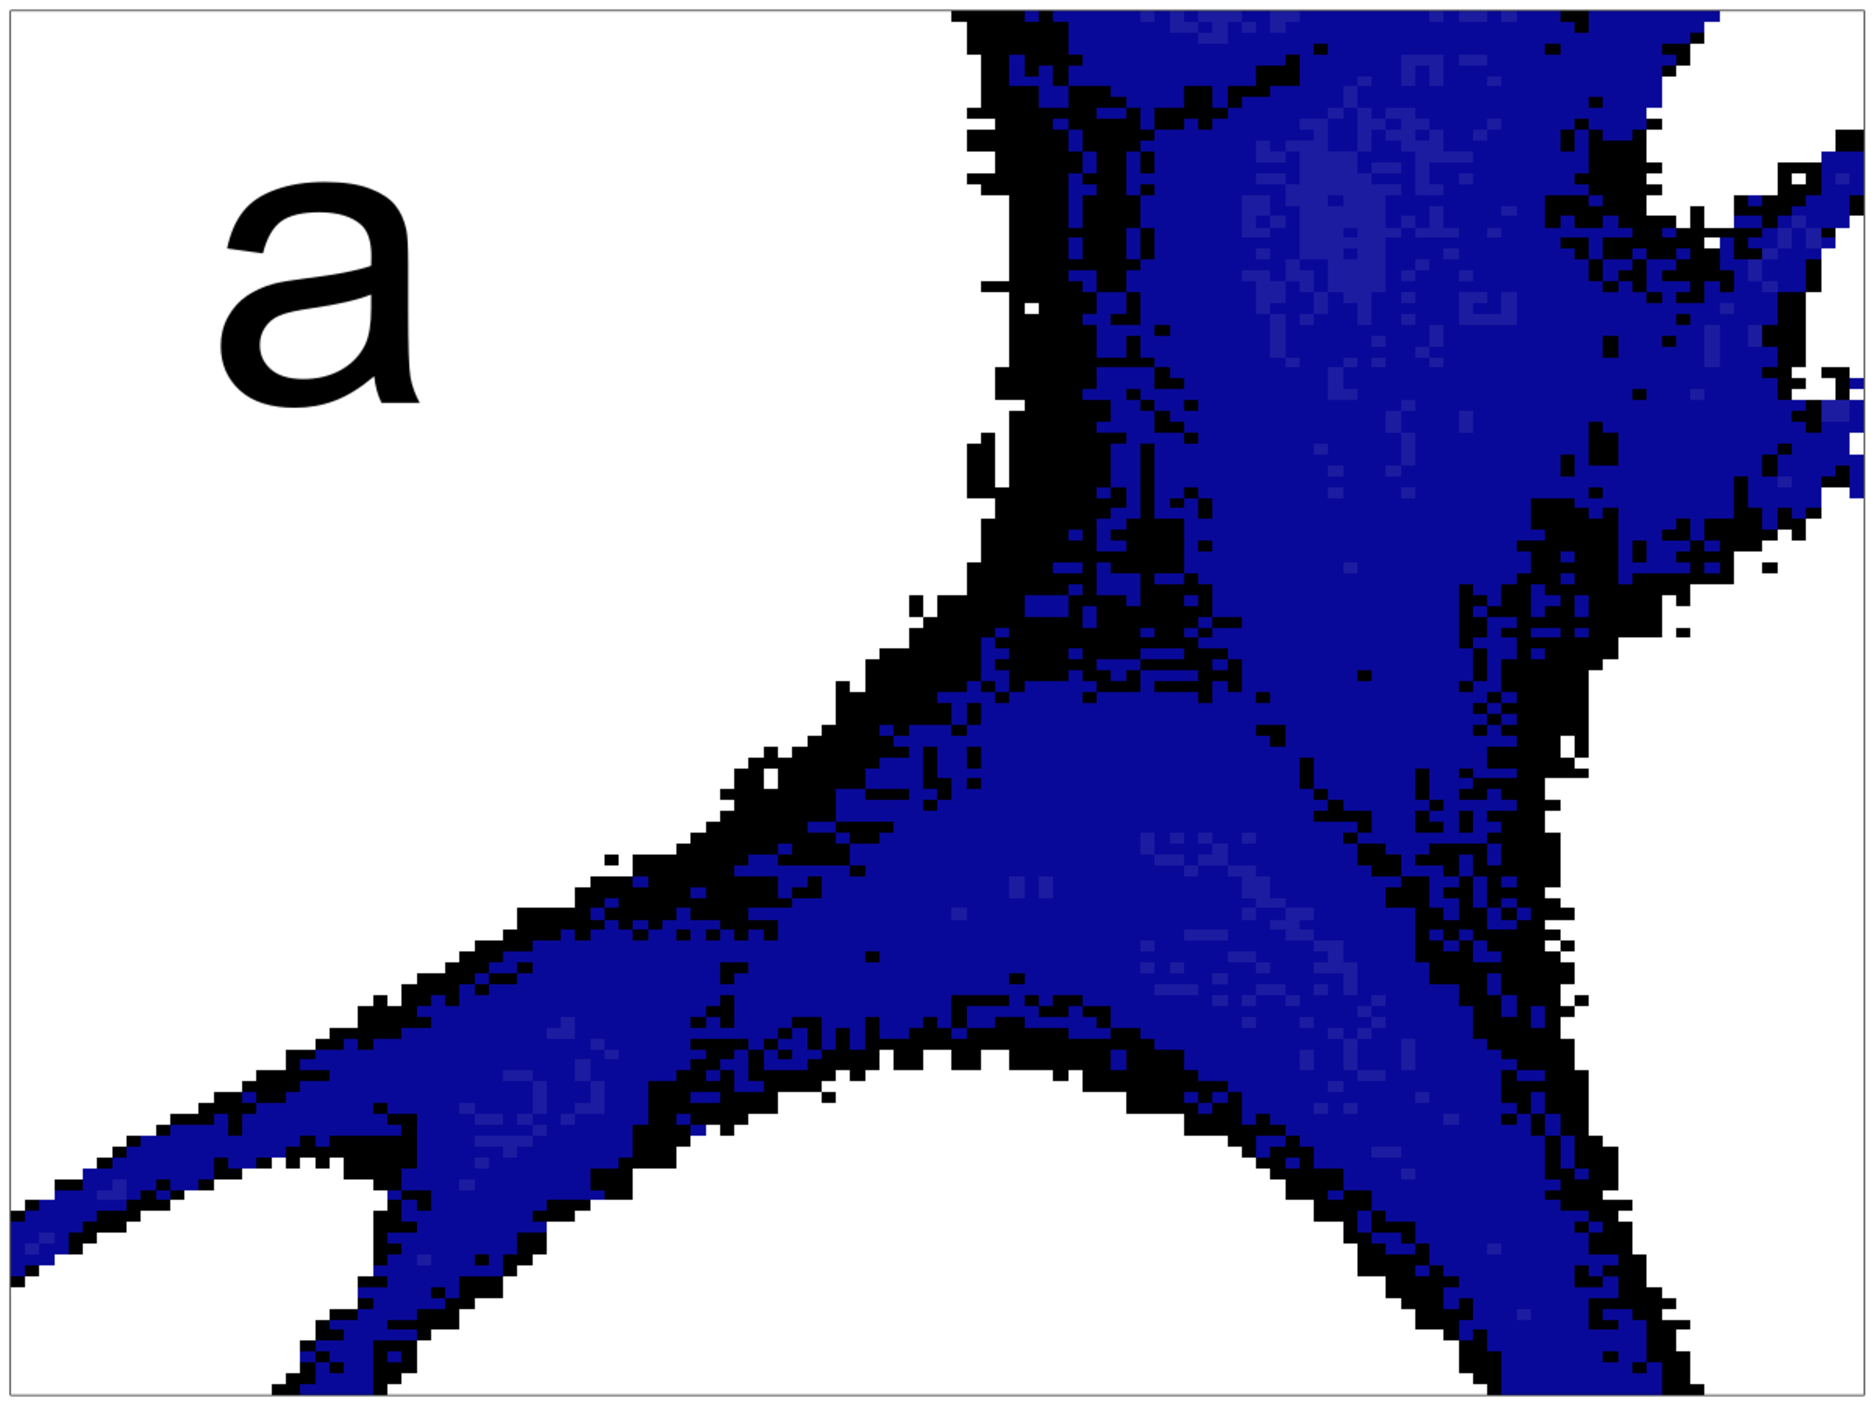
\includegraphics[width=0.32\textwidth]{m5}
		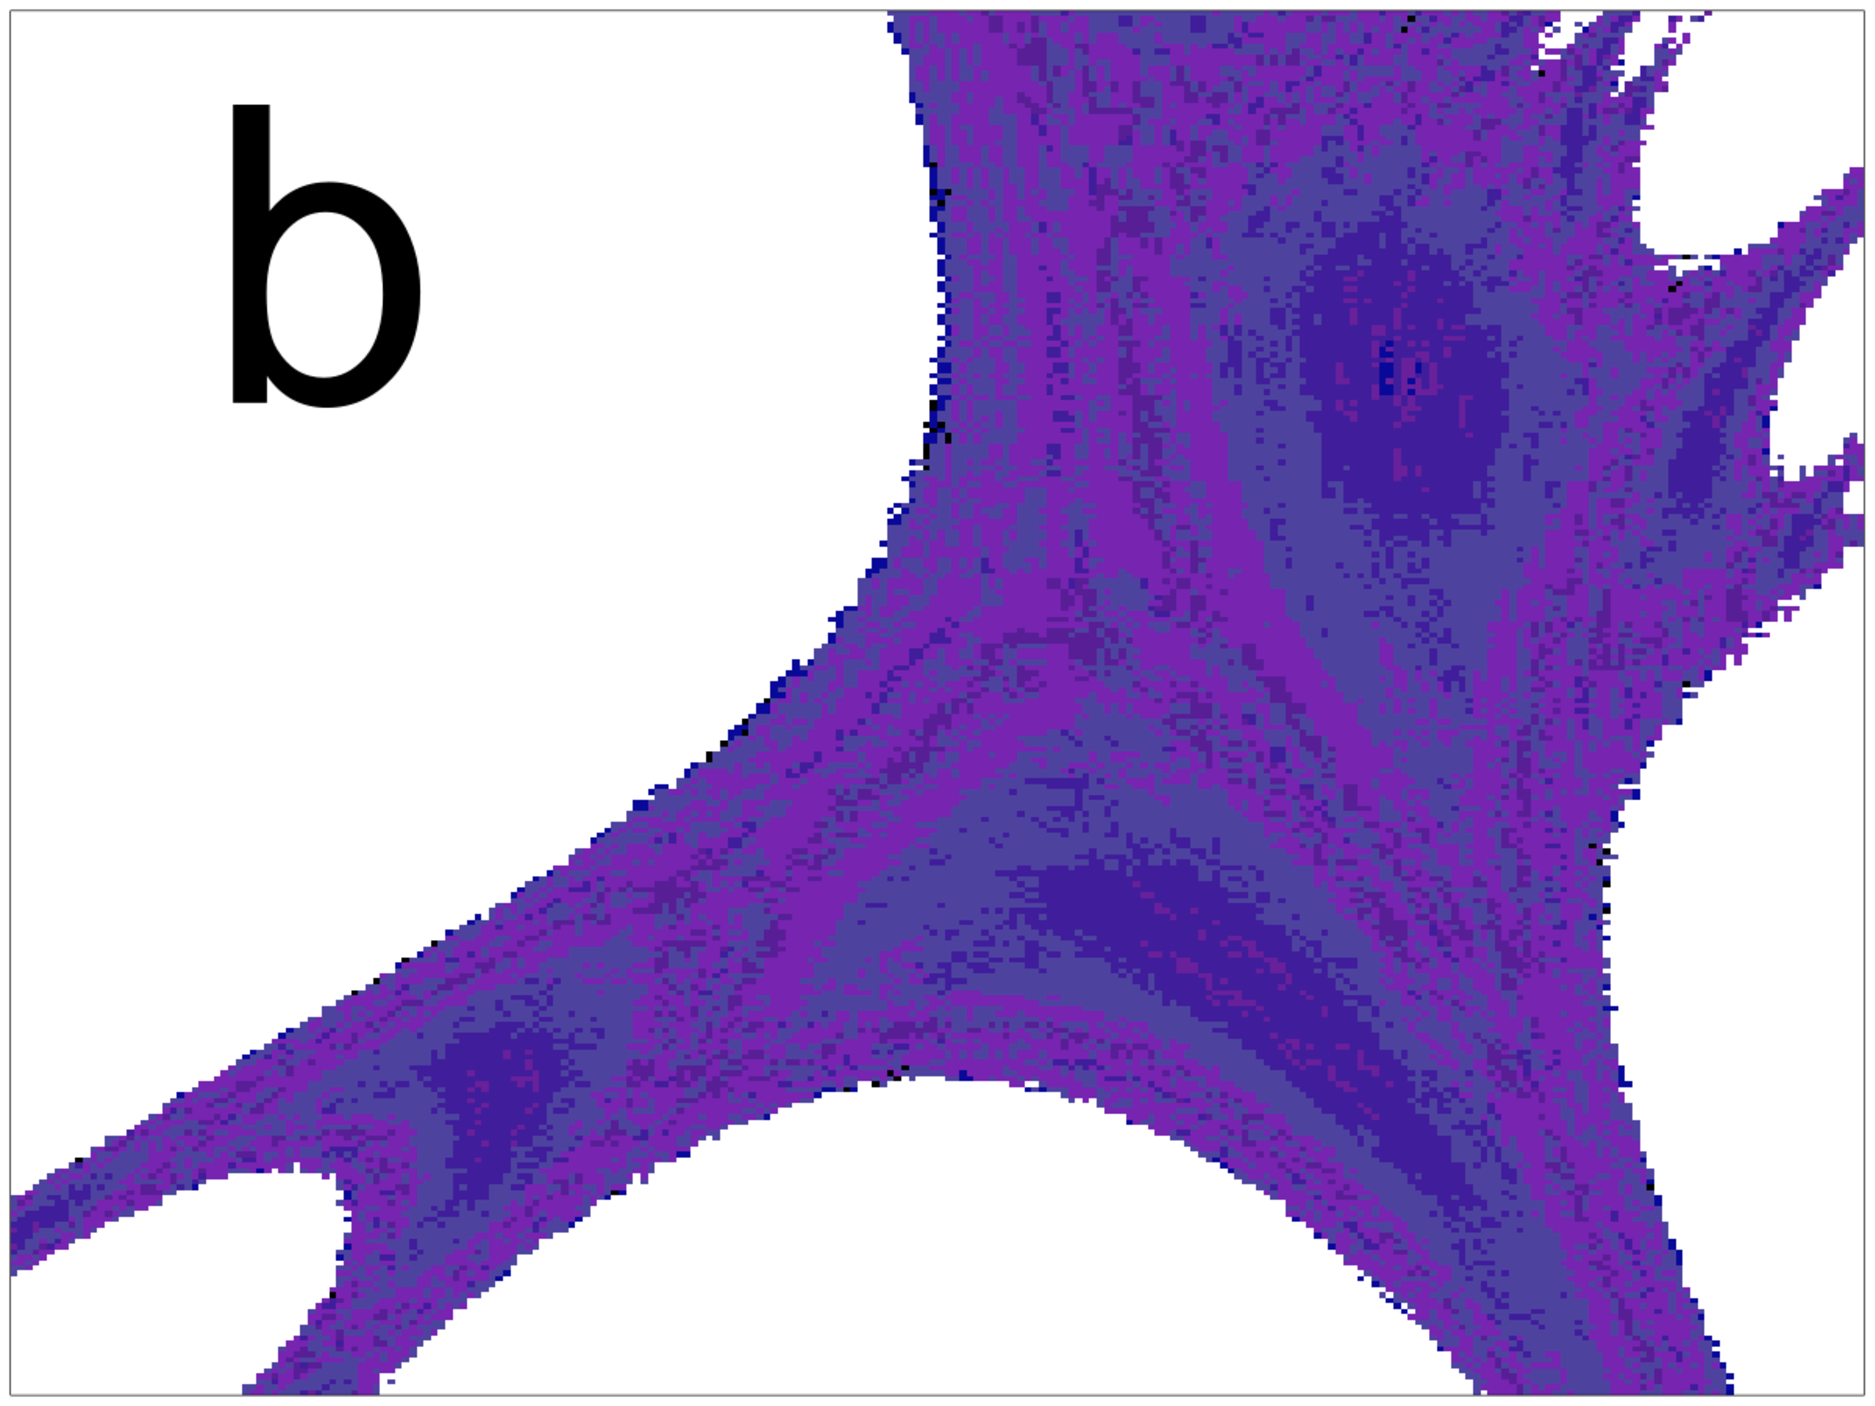
\includegraphics[width=0.32\textwidth]{m6}
		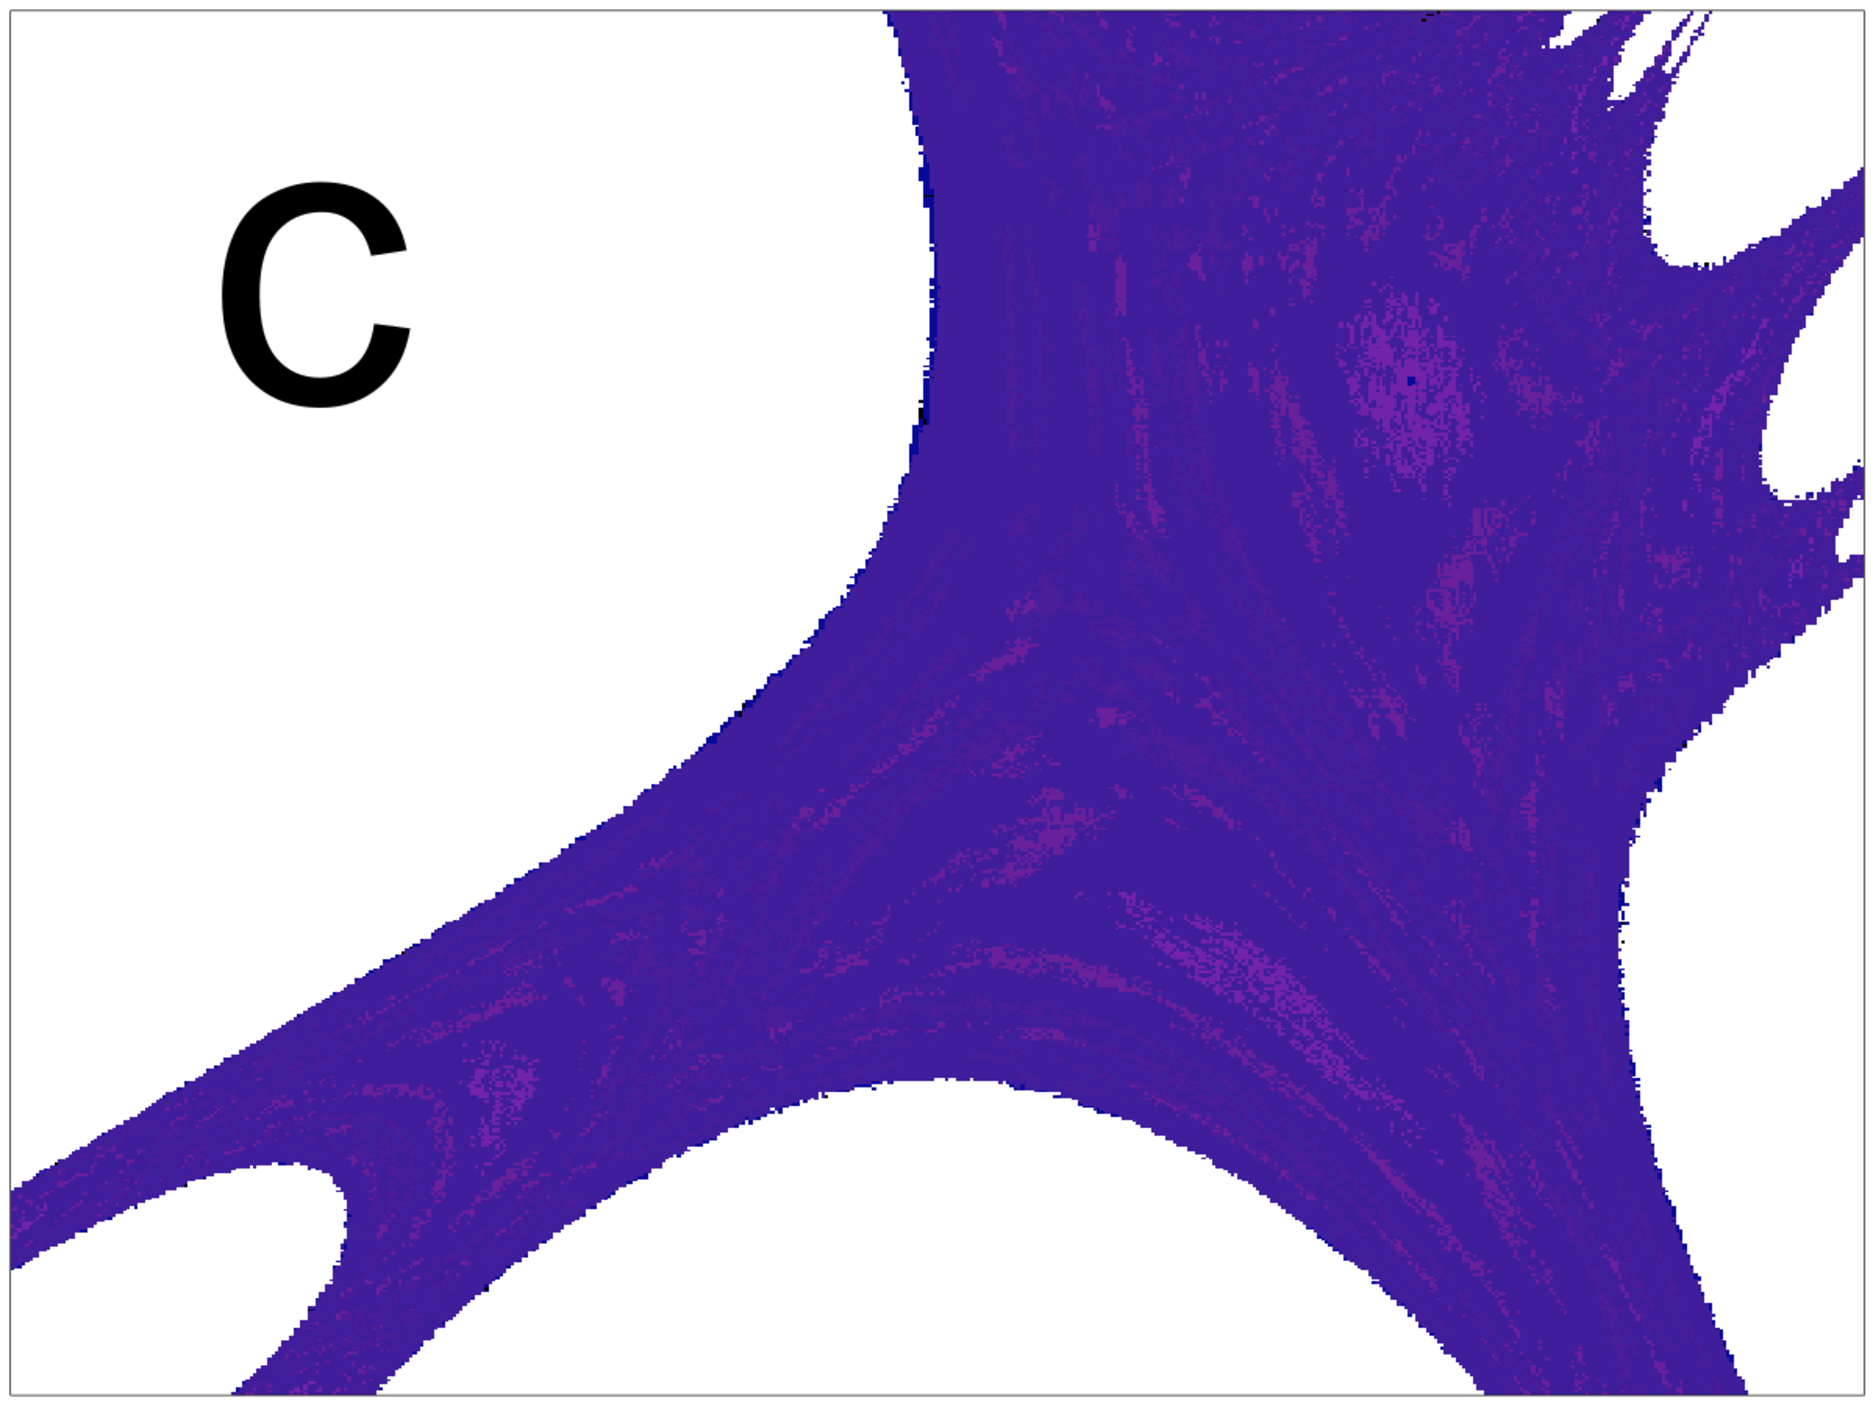
\includegraphics[width=0.32\textwidth]{m7}\\
		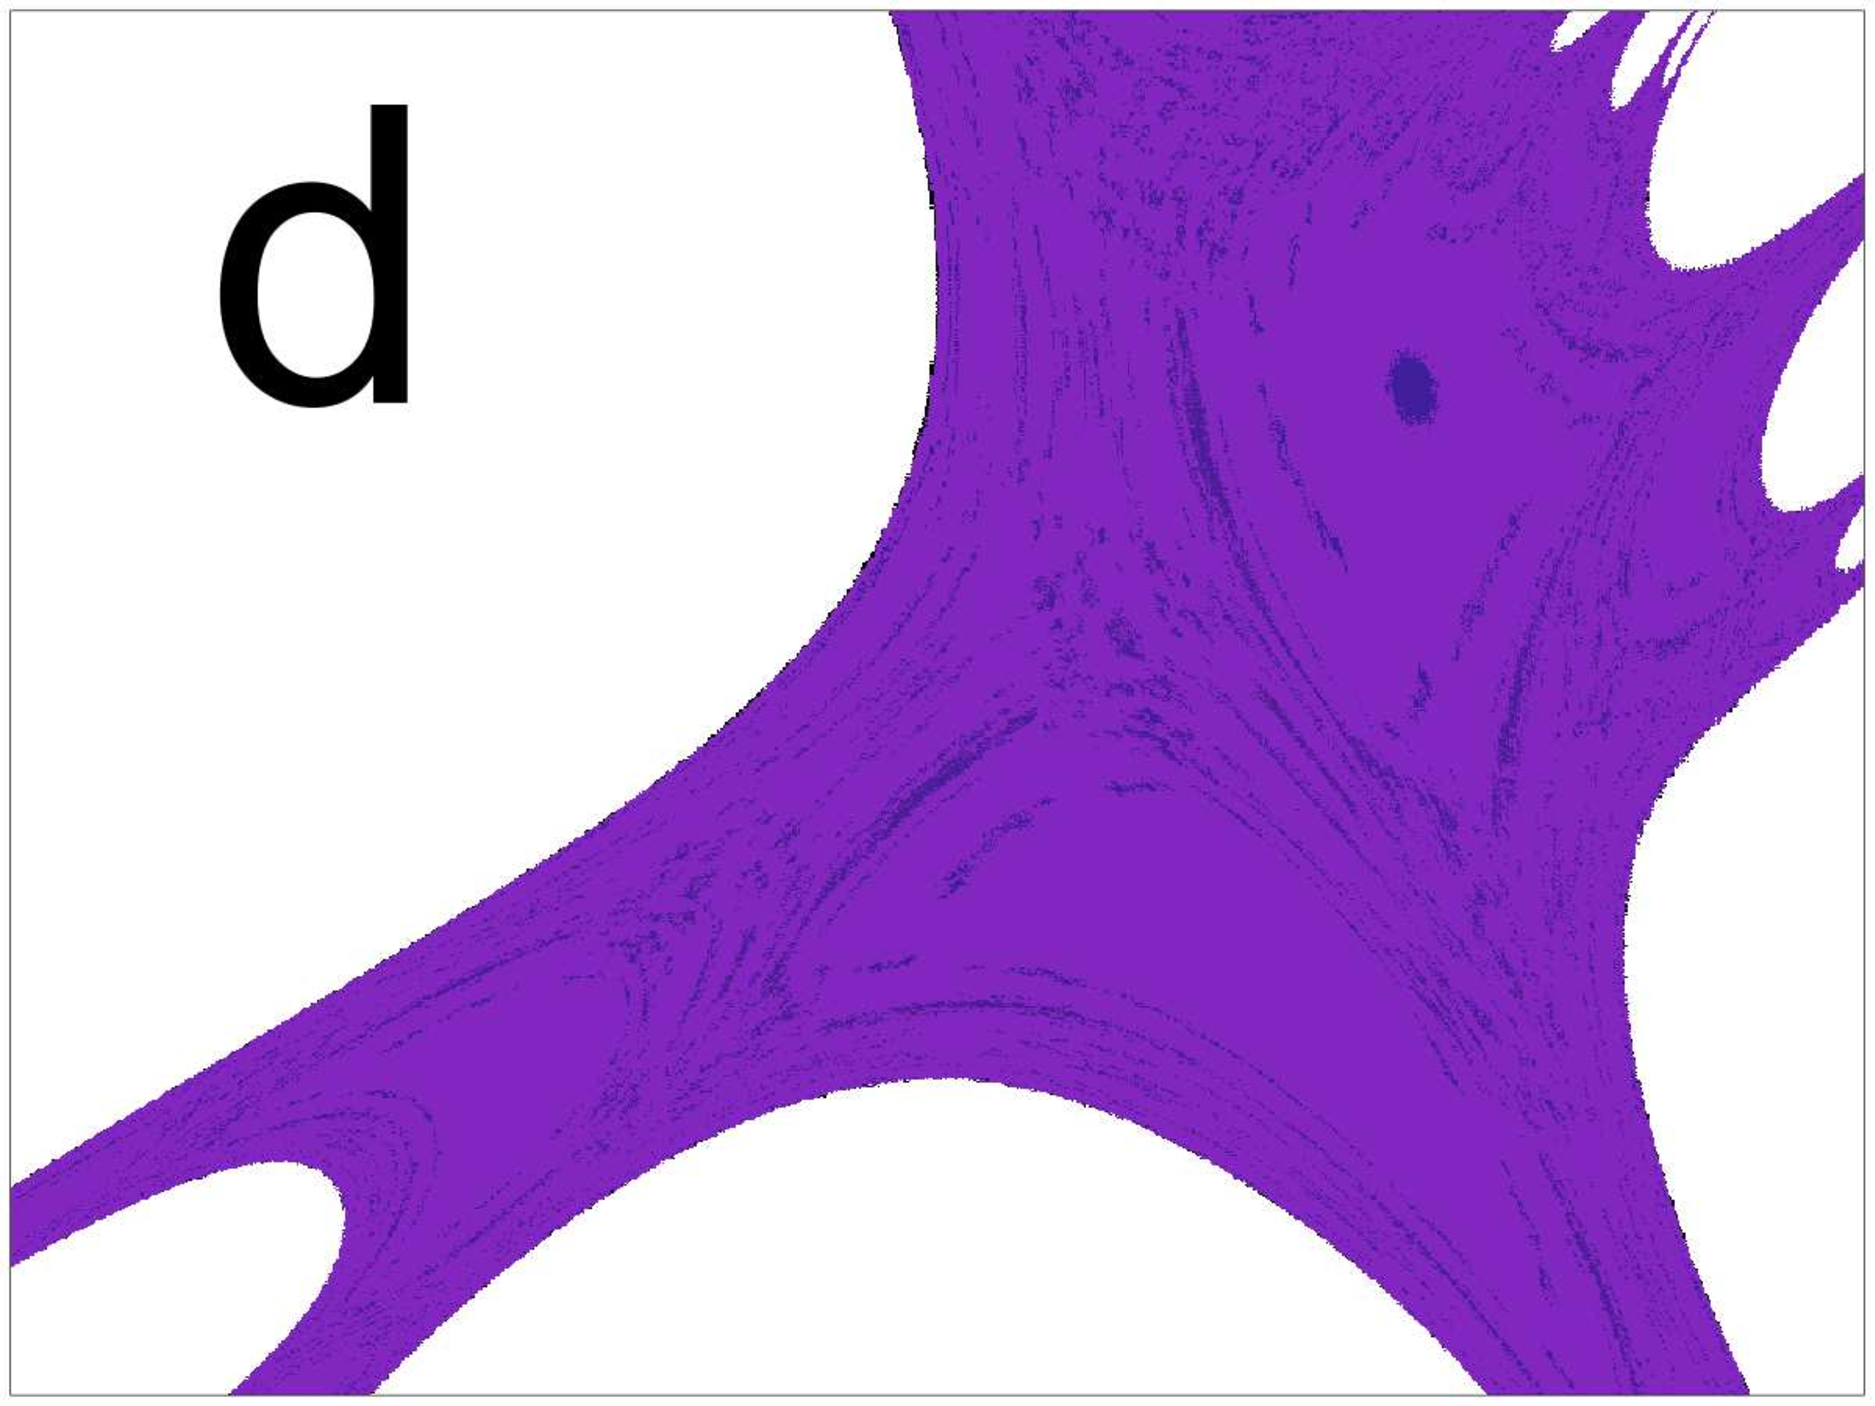
\includegraphics[width=0.32\textwidth]{m8}
		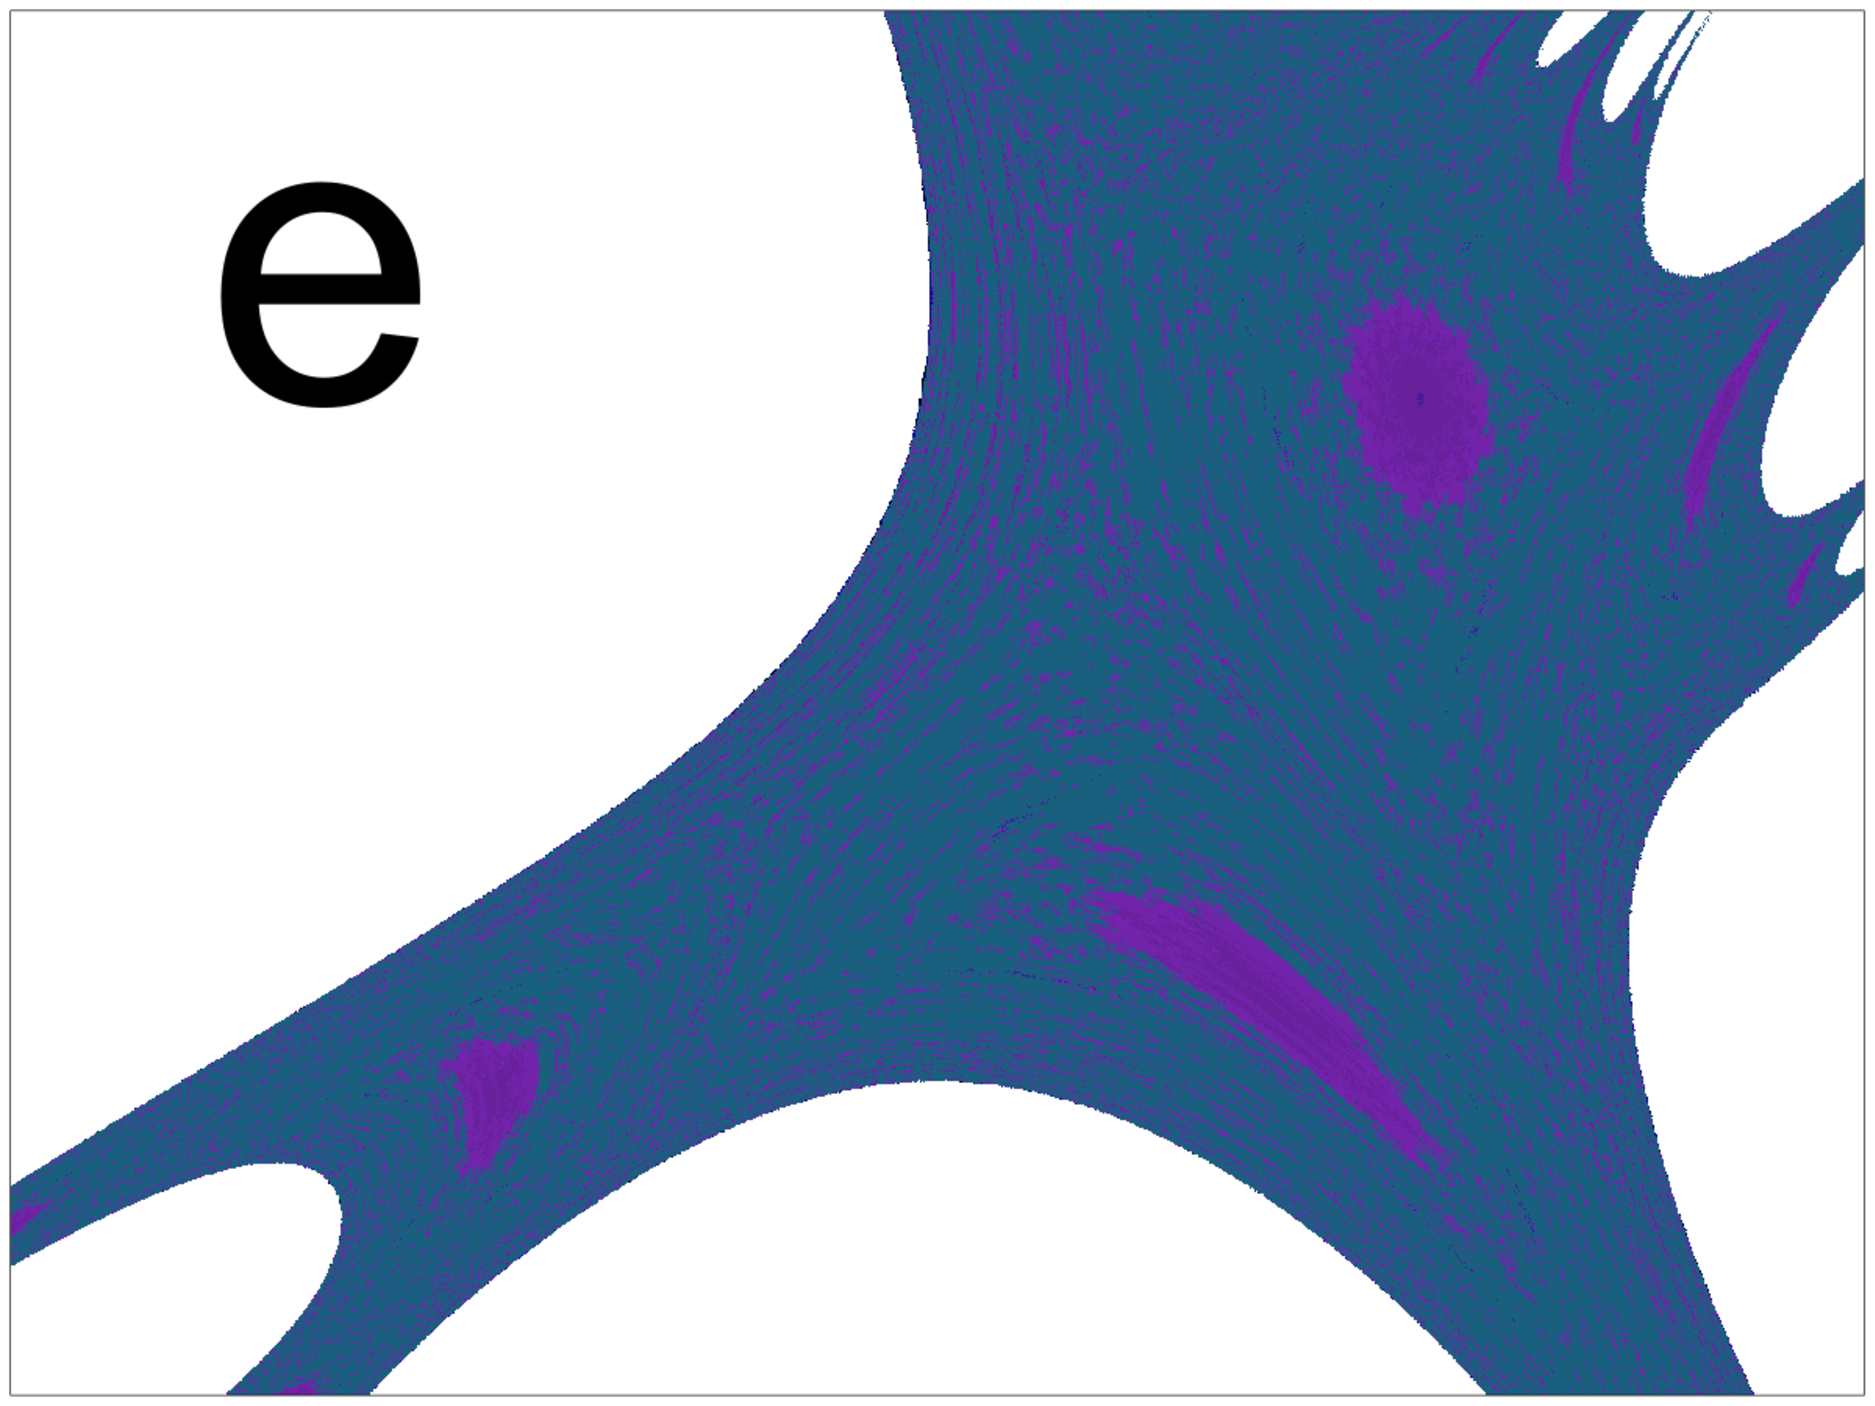
\includegraphics[width=0.32\textwidth]{m9}
		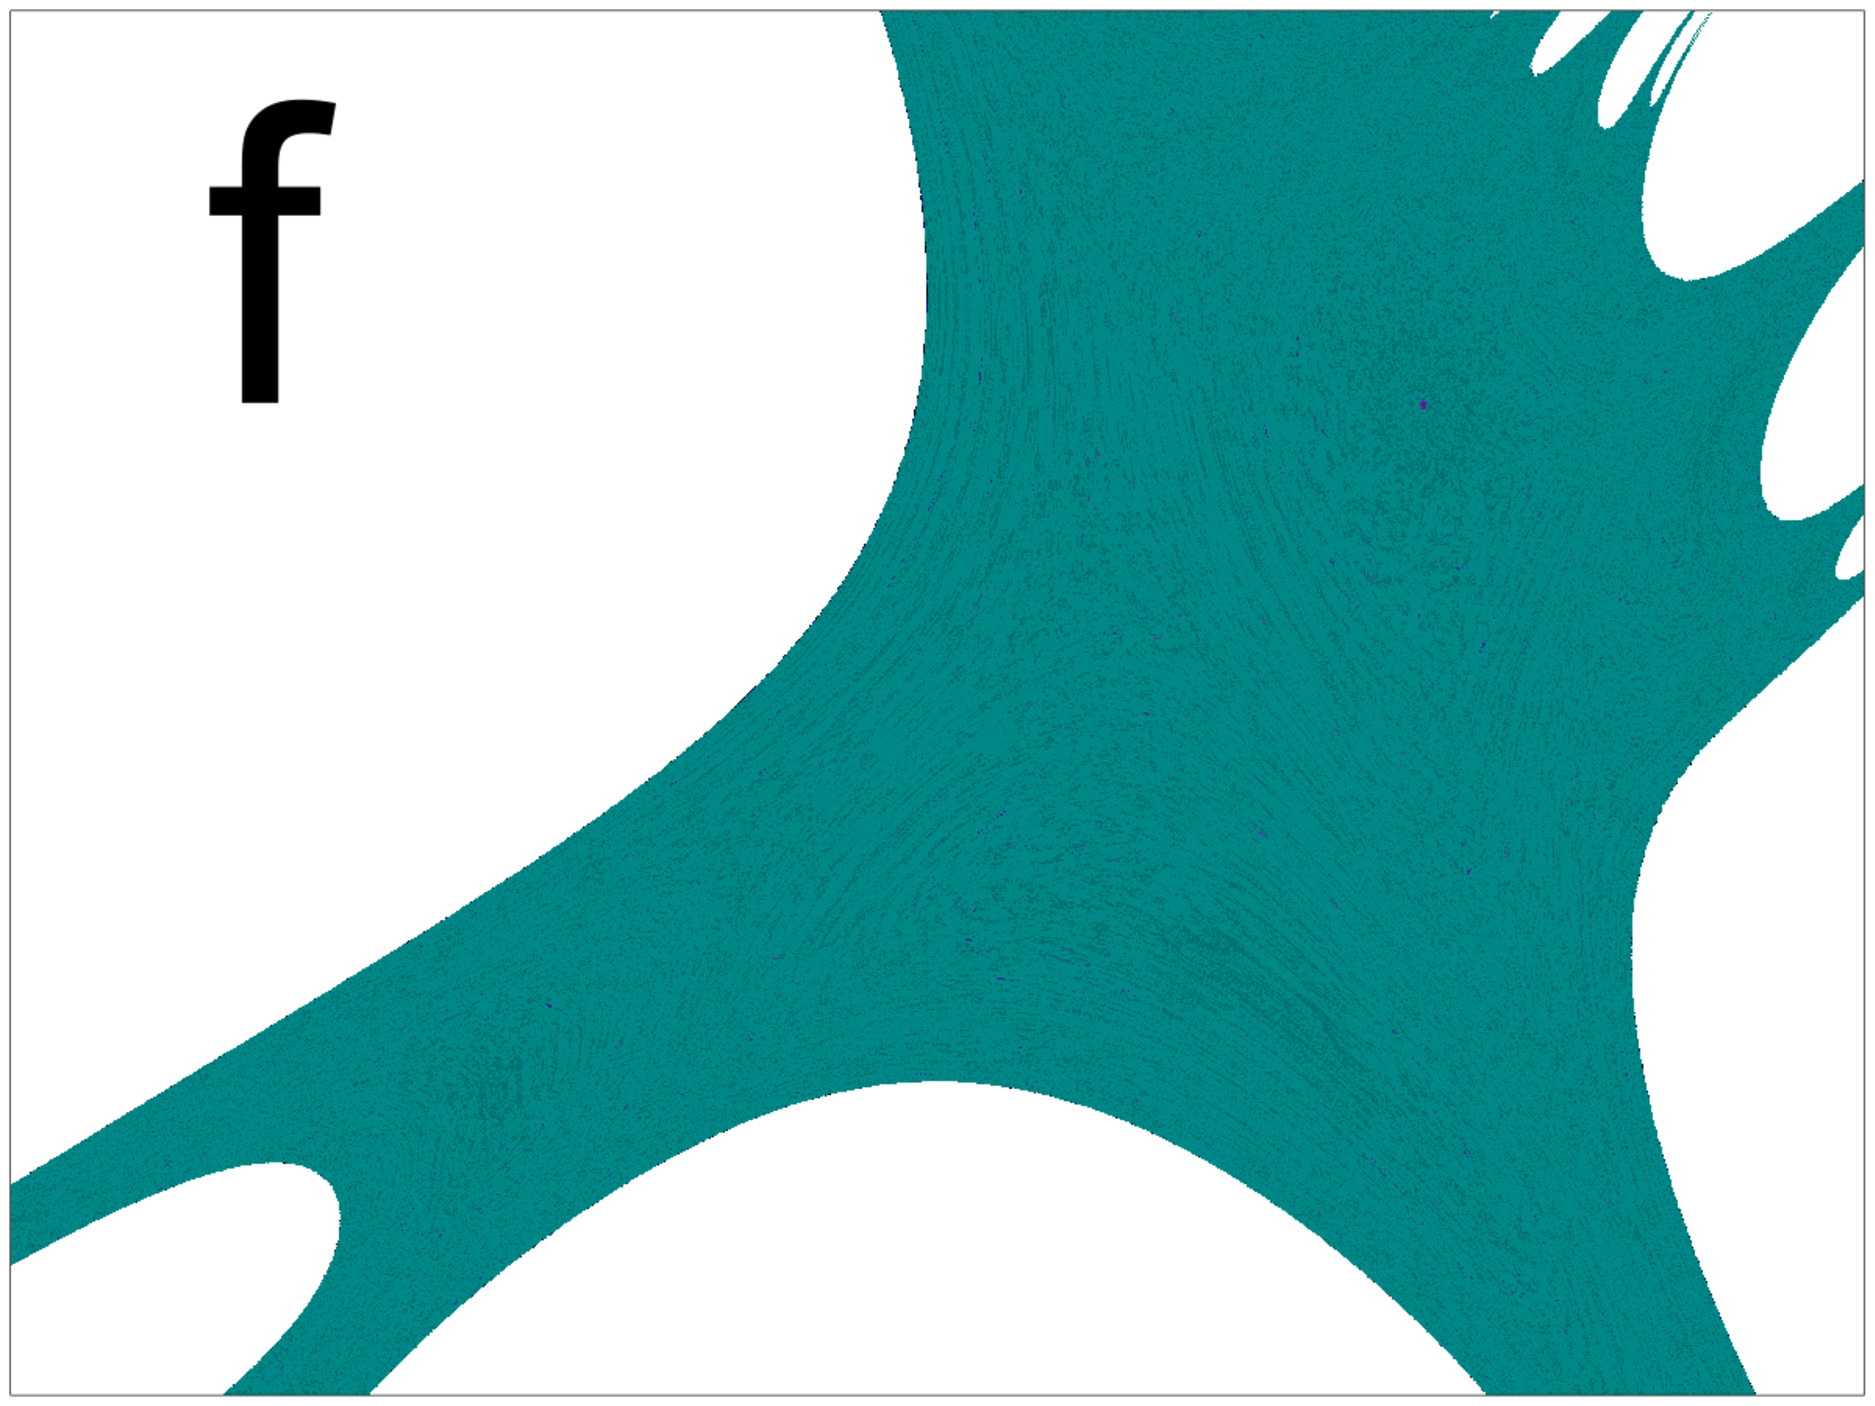
\includegraphics[width=0.32\textwidth]{m10}\\
		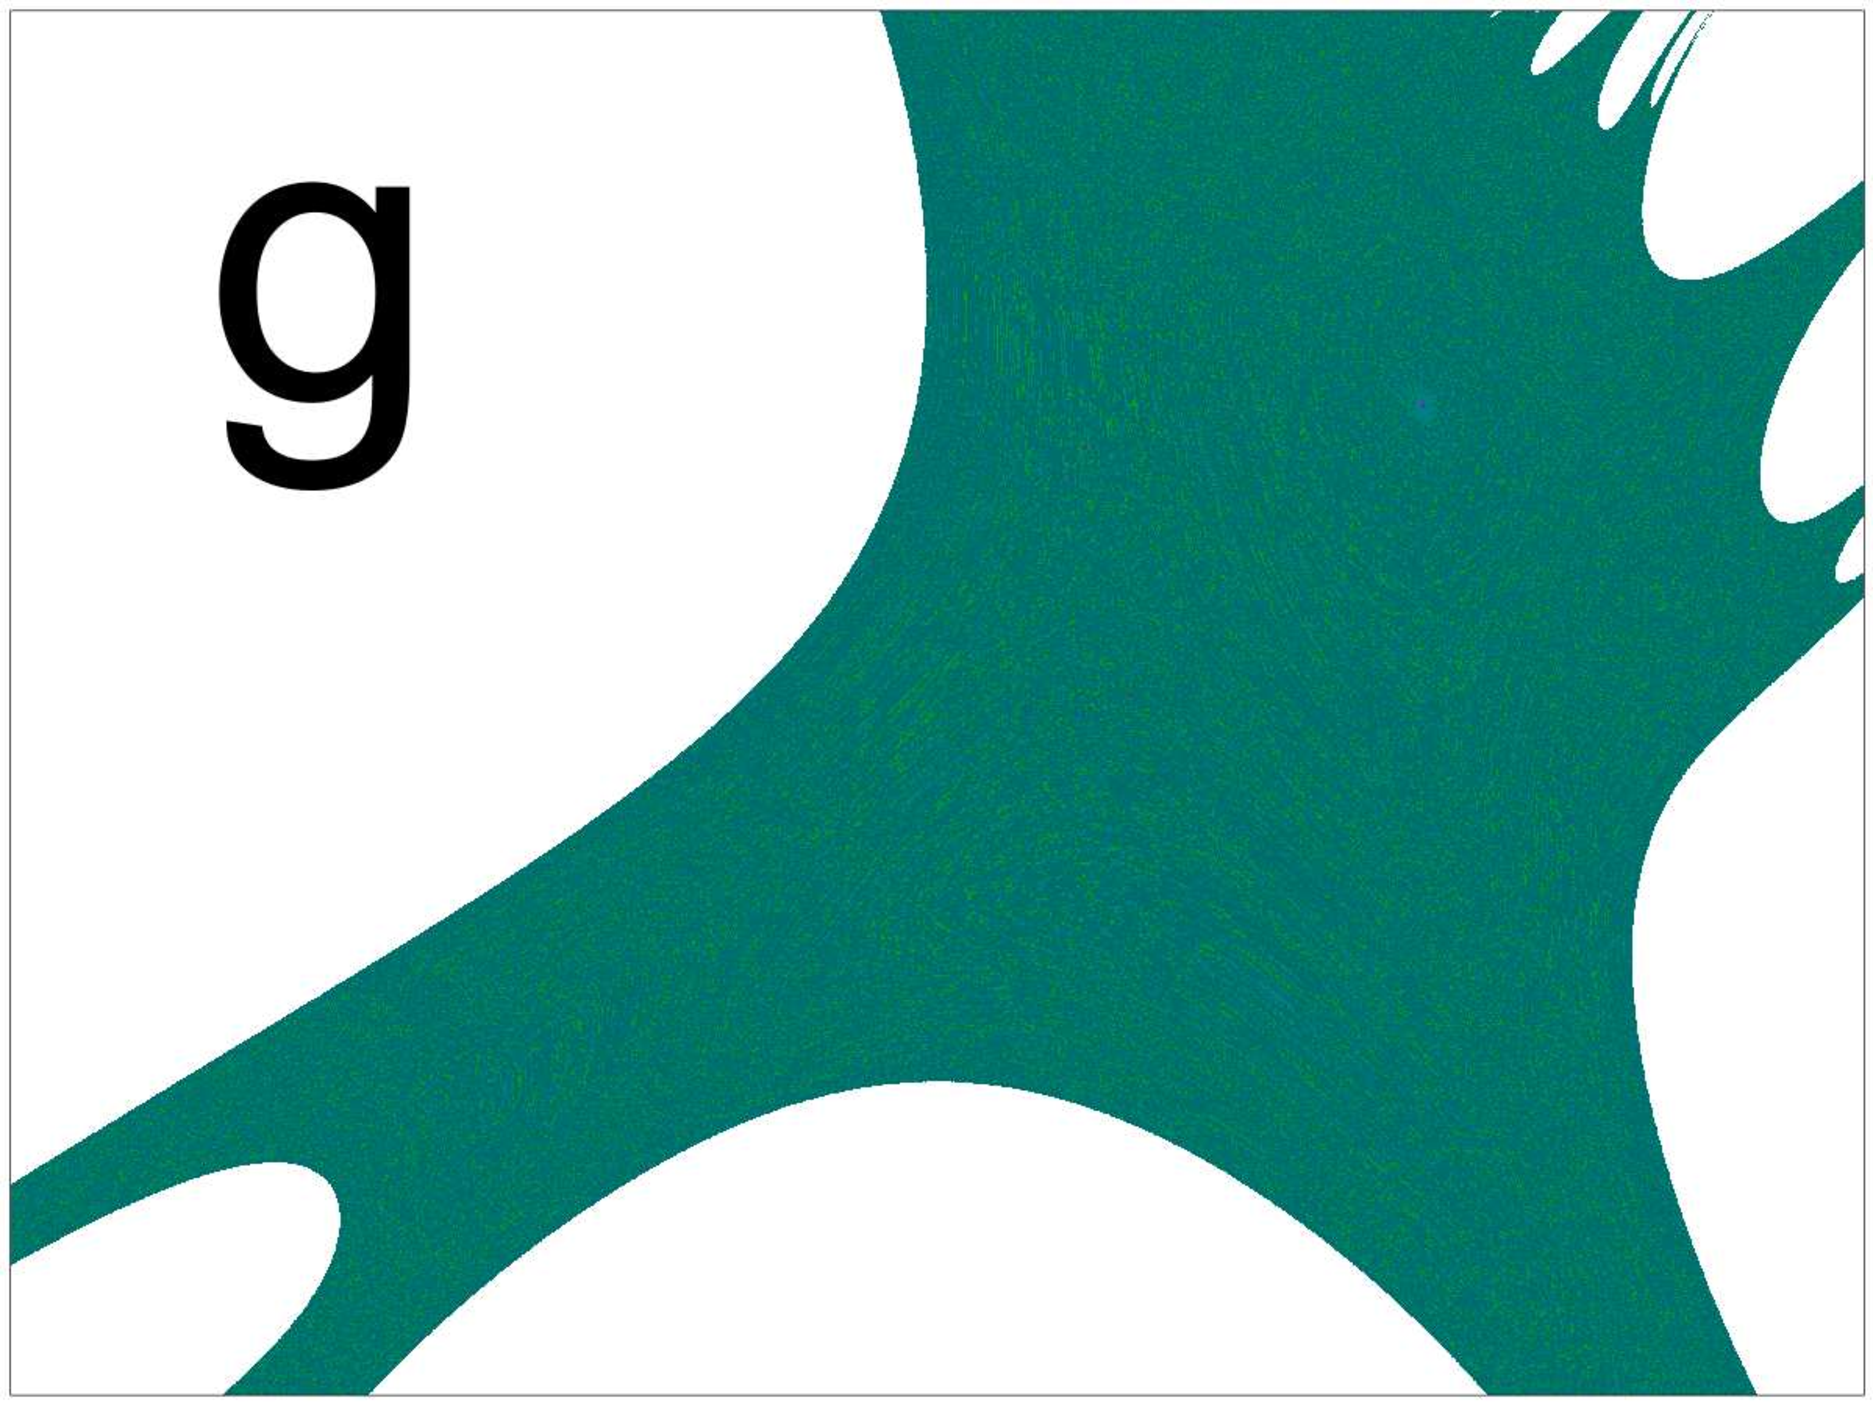
\includegraphics[width=0.32\textwidth]{m11}
		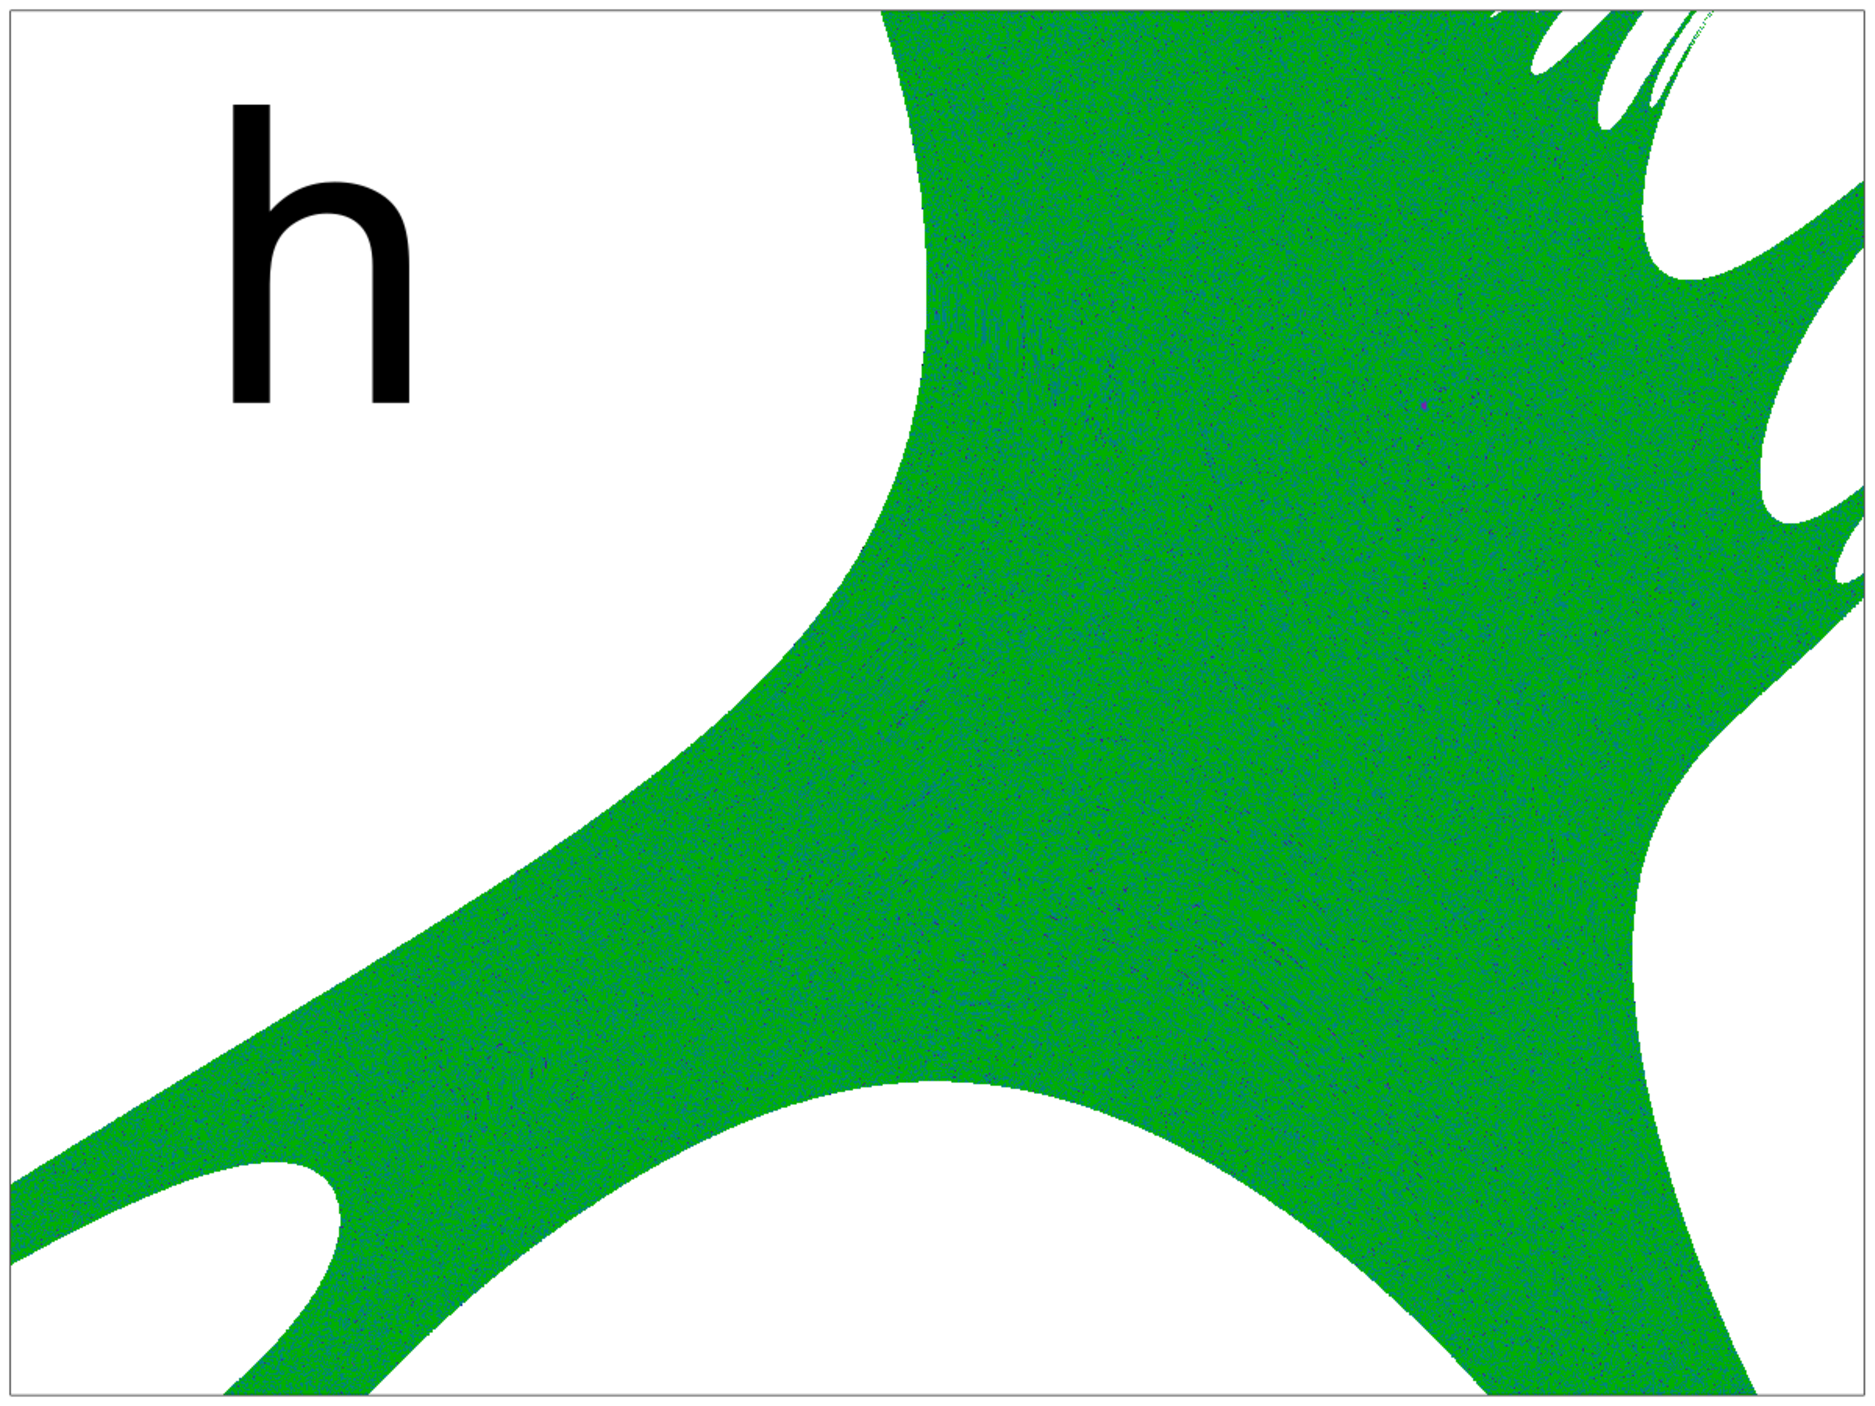
\includegraphics[width=0.32\textwidth]{m12}
		
\includegraphics[width=0.32\textwidth]{m13}\\
		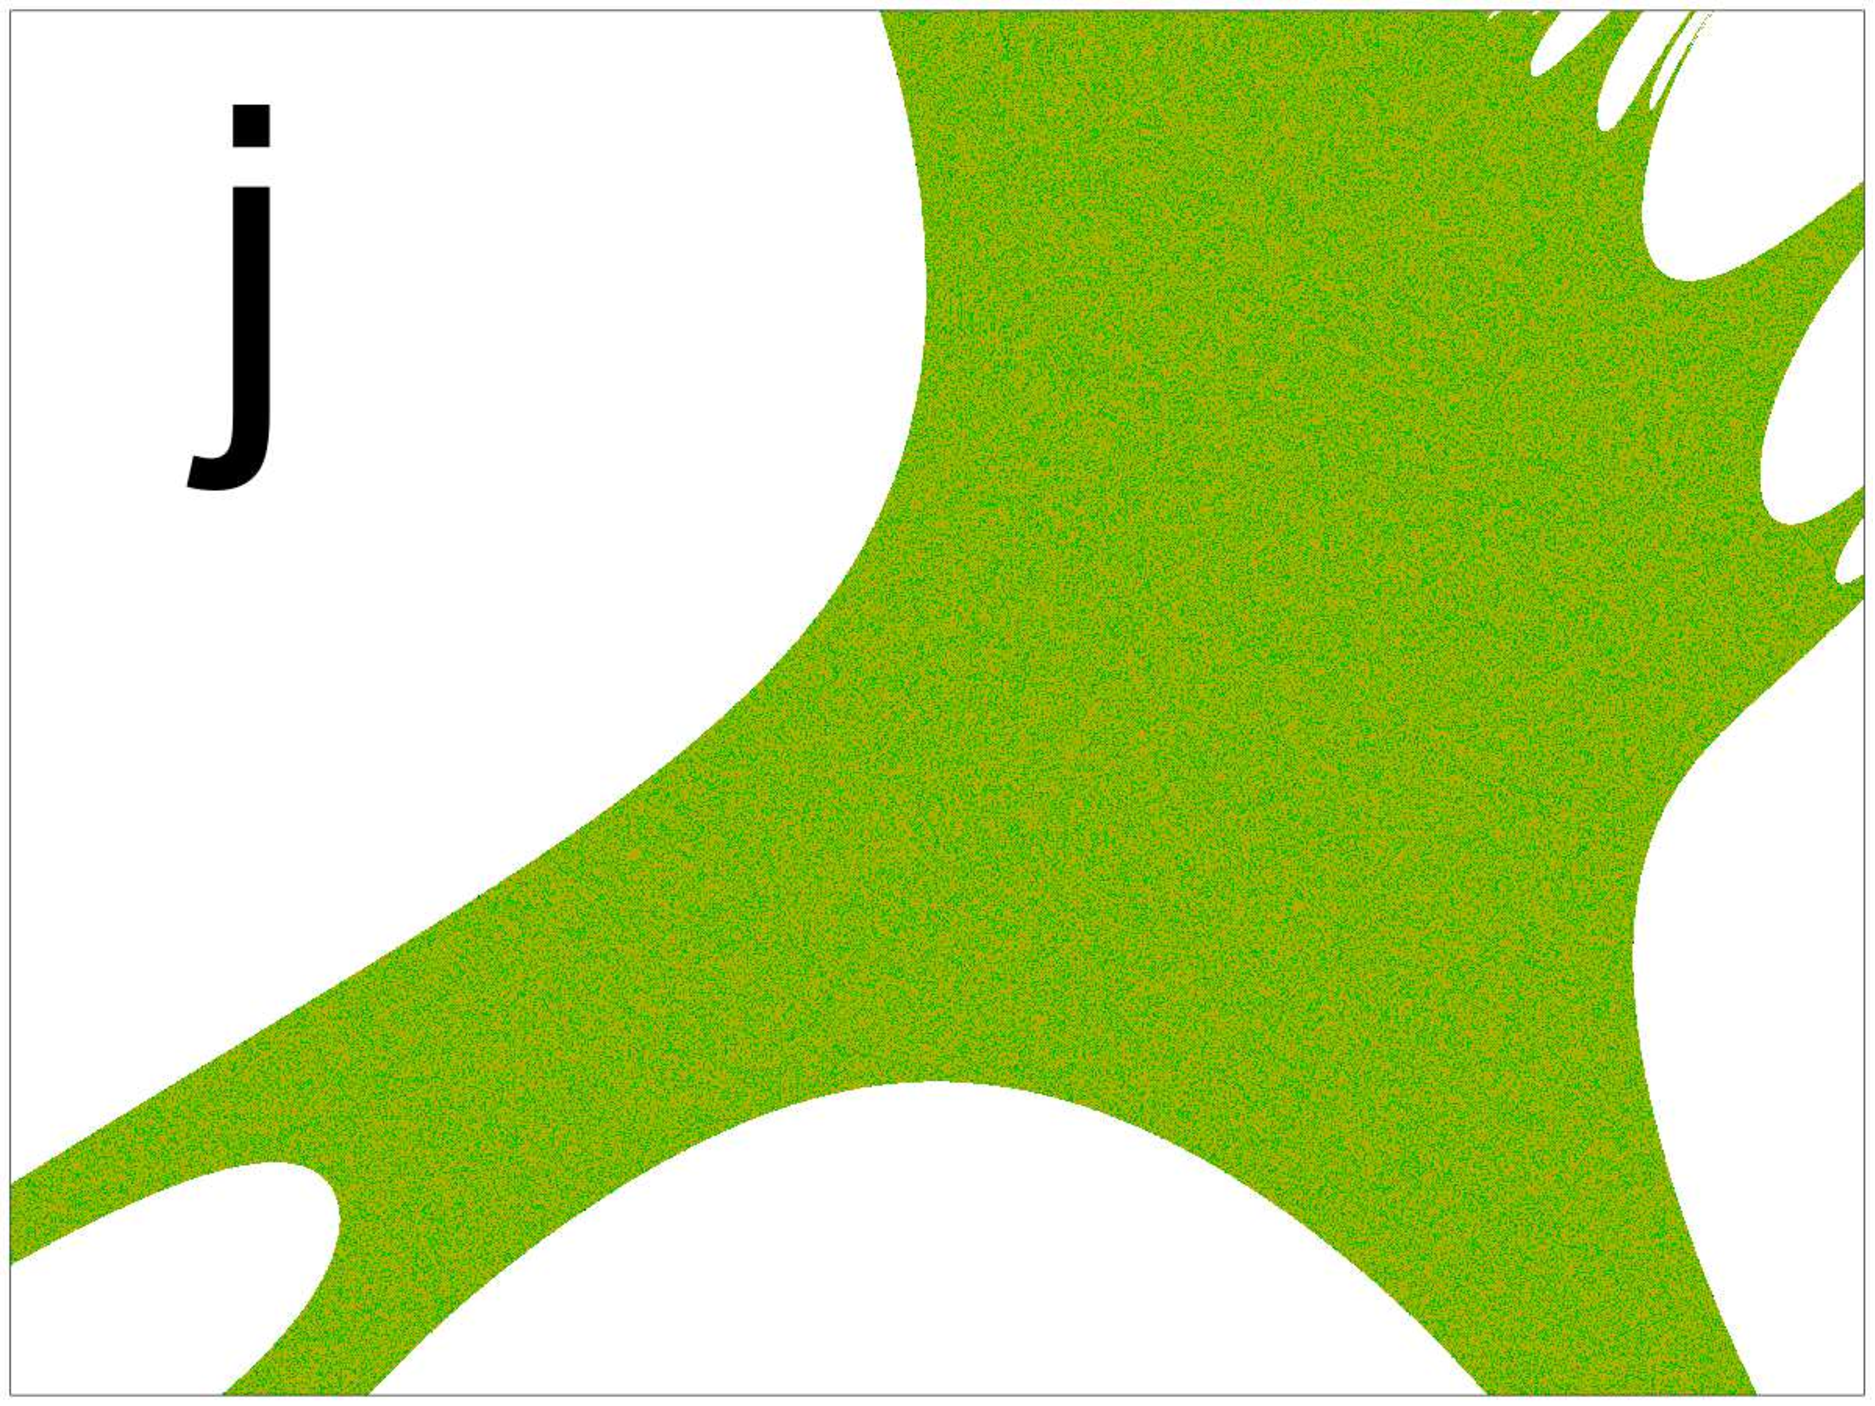
\includegraphics[width=0.32\textwidth]{m14}
		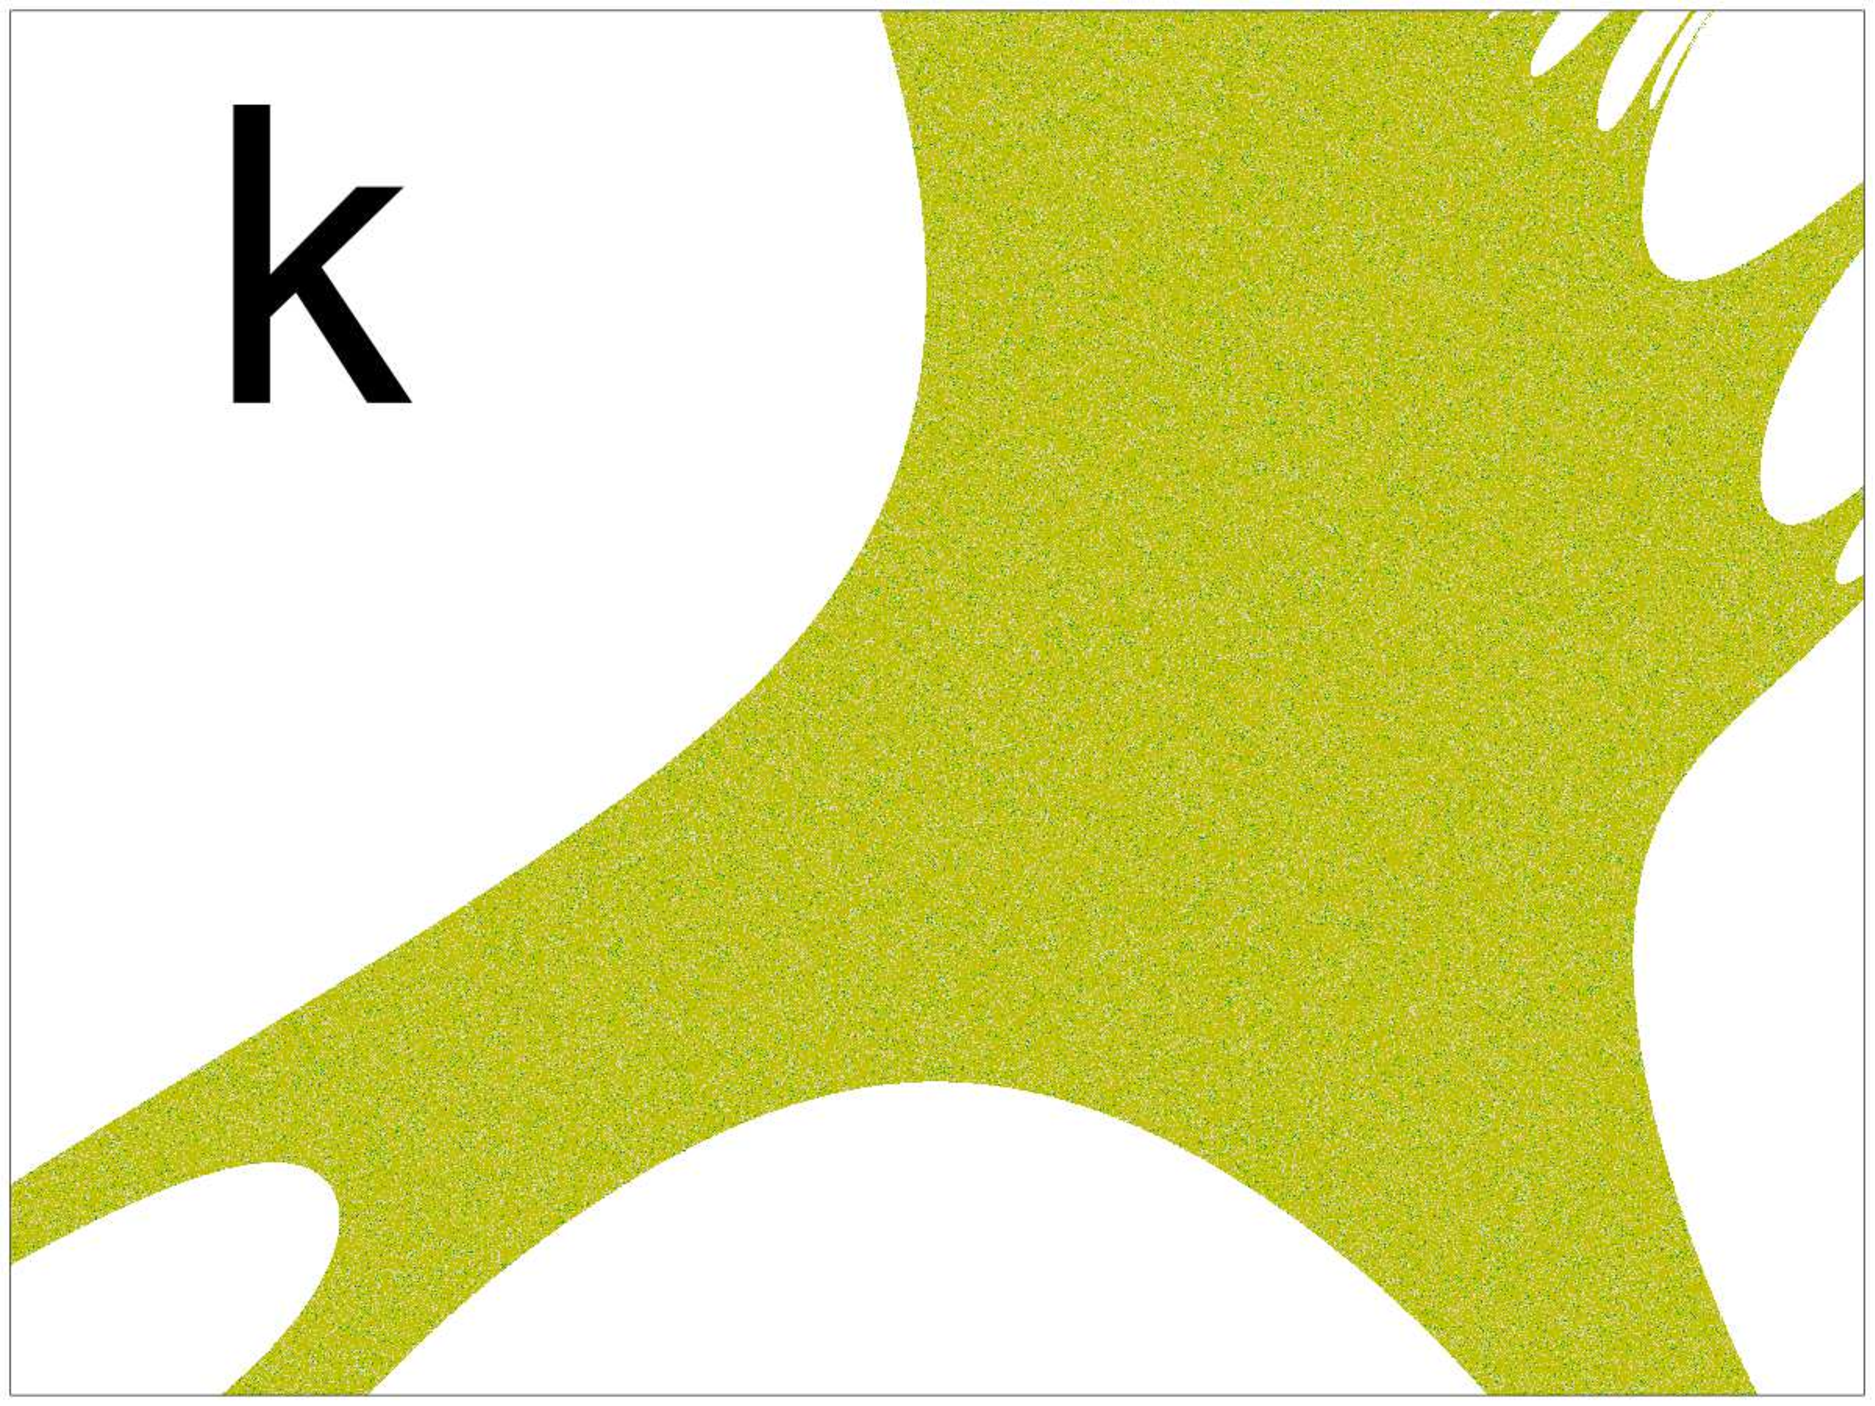
\includegraphics[width=0.32\textwidth]{m17}
		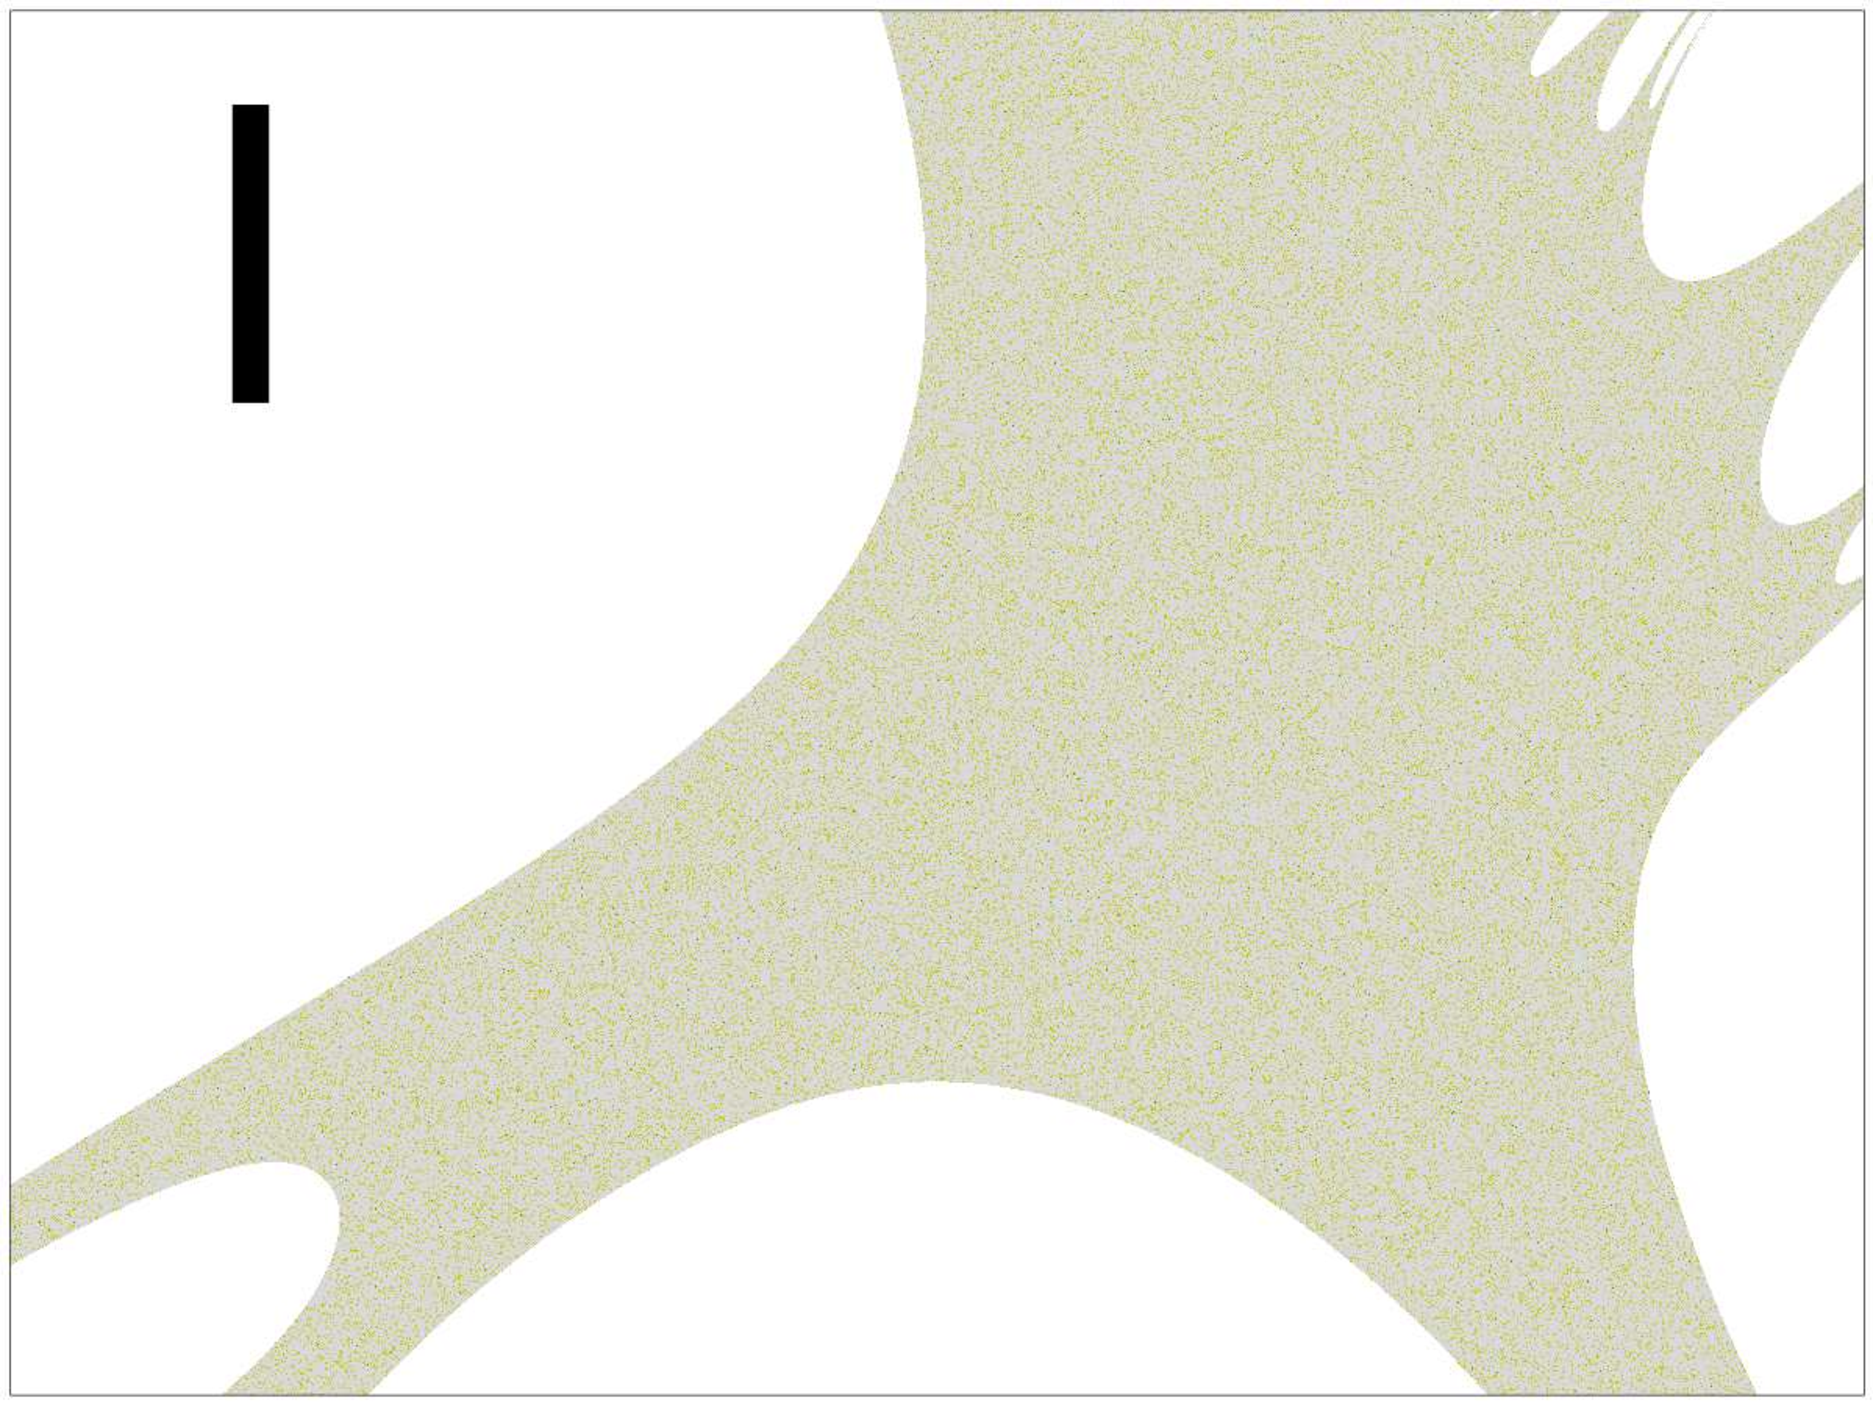
\includegraphics[width=0.32\textwidth]{m18}\\
		\\   
		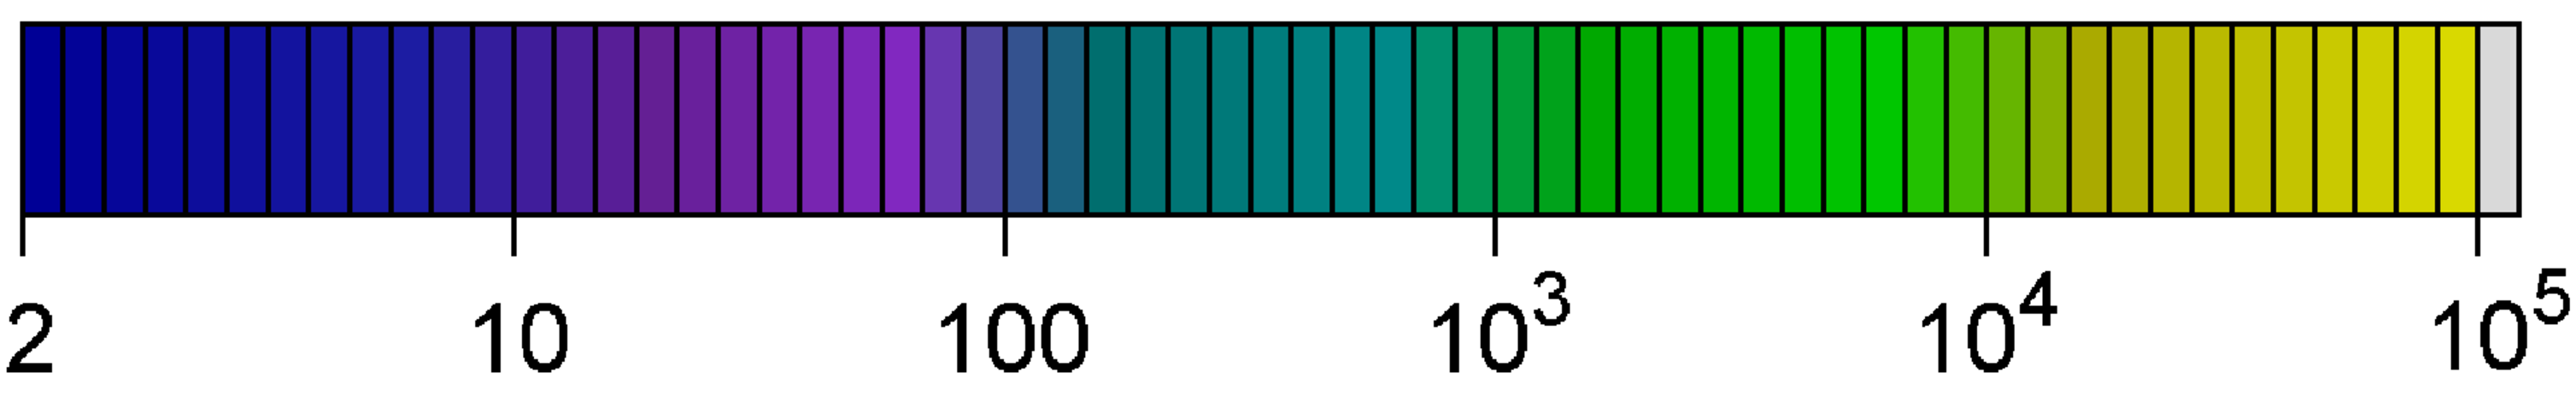
\includegraphics[width=0.75\textwidth]{ColorMapConEje}
	\end{tabular}
	\caption{Evolución de las longitudes de período de los dominios de atracción para: (a) $n_f=5$, (b) $n_f=6$, (c) $n_f=7$, (d) $n_f=8$, (e) $n_f=9$, (f) $n_f=10$, (g) $n_f=11$, (h) $n_f=12$, (i) $n_f=13$, (j) $n_f=14$, (k) $n_f=17$, (l) $n_f=18$.}
	\label{fig:m}
\end{figure*}

La Figura \ref{fig:m} muestra que a medida que aumenta el valor de $n_f$ el color del área se vuelve más uniforme y claro, lo que indica que las CIs convergen a ciclos de períodos más largos.
Esto también se puede ver en el Cuadro \ref{tabla}, donde a medida que $n_f$ aumenta, la longitud del ciclo límite predominante también aumenta.

Para comparar los valores obtenidos con las secuencias reales, se iteraron los atractores en punto flotante con mantisa de $236$ bits (IEEE754 de punto flotante binario de precisión óctuple) lo que aquí se llamó \textit{punto flotante} o simplemente \textit{flotante}, es la aritmética más cercana a los números reales a la que podemos acceder con tiempos de cómputo razonables.
Se puede observar que cuando se empleó la precisión mencionada, todos los períodos resultaron ser superiores a $10 ^ 5$ y convergieron al atractor caótico que se ve en la Figura \ref{fig:atractores3592}.d.

\begin{table*}[!t]
	% increase table row spacing, adjust to taste
	\renewcommand{\arraystretch}{1.3}
	\caption{Longitudes de períodos dentro del dominio de atracción $x$ e $y$ $\epsilon$  $[-2,2]$.}
	\label{tabla}
	\centering
	\fontsize{9}{9}\selectfont
	\begin{tabular}{l  l  }
		\hline
		$n_f$   & $T$ {\scriptsize(Porcentage de CIs que convergen a esta longitude deperíodo)}\\ \hline\hline
		$5$     & $2$ {\scriptsize($92.7\%$ )};$6$  {\scriptsize($7.3\% )$}                                                                                                                                                                  \\
		$6$     & $88$ {\scriptsize($41.6 \% )$};$44$ {\scriptsize($36.7 \% )$};$12$ {\scriptsize($13.8\% )$};$16$ {\scriptsize($6.2 \% )$};$2$ {\scriptsize($0.8 \% )$};$24$ {\scriptsize($0.6 \% )$};$26$ {\scriptsize($0.2 \%)$}          \\
		$7$     & $12$ {\scriptsize($83.5 \% )$};$14$ {\scriptsize($8.9\% )$};$24$ {\scriptsize($5.2\% )$};$34$ {\scriptsize($1.8 \% )$};$2$ {\scriptsize($0.6\% )$}                                                                         \\
		$8$     & $68$ {\scriptsize($91.7\%)$};$14$ {\scriptsize($6.2\%)$};$12$ {\scriptsize($1.8 \%)$};$17$ {\scriptsize($0.2\% )$};$15$ {\scriptsize($0.1 \%)$}                                                                            \\
		$9$     & $140$ {\scriptsize($54.5 \%)$};$123$ {\scriptsize($25.4 \%)$};$34$ {\scriptsize($8.6\%)$};$44$ {\scriptsize($4.3 \%)$};$38$ {\scriptsize($3.9 \%)$};$22$ {\scriptsize($2.9 \%)$};$48$;$2$;$12$;$4$ {\scriptsize($<0.1\%)$} \\
		$10$    & $655$ {\scriptsize($78.2\%)$};$212$ {\scriptsize($21.1\%)$};$143$ {\scriptsize($0.5\%)$};$12$ {\scriptsize($0.1\%)$};$2$;$36$;$13$;$20$;$10$;$4$ {\scriptsize($<0.1\%)$}                                                   \\
		$11$    & $153$ {\scriptsize($78.1\%)$};$461$ {\scriptsize($10.8\% )$};$1381$ {\scriptsize($8.7\%)$};$434$ {\scriptsize($2.3\%)$};$18$;$30$;$53$;$32$;$34$;$10$;$2$ {\scriptsize($<0.1\% )$}                                         \\
		$12$    & $2,278$ {\scriptsize($64.4\%)$};$438$ {\scriptsize($22.4\% )$};$598$ {\scriptsize($7.6\% )$};$886$ {\scriptsize($4.7 \%)$};$12$ {\scriptsize($0.7\%)$};$87$;$2$;$42$;$23$;$32$;$10$ {\scriptsize($<0.1\% )$}               \\
		$13$    & $11,510$ {\scriptsize($ 98.9\%)$};$1052$ {\scriptsize($1 \%)$};$12$;$26$;$2$;$10$ {\scriptsize($<0.1\% )$}                                                                                                                 \\
		$14$    & $21,333$ {\scriptsize($69.2\% )$};$5.804$ {\scriptsize($16.5\%  )$};$4,795$ {\scriptsize($7.9\%  )$};$1,264$ {\scriptsize($5.8 \% )$};$2,429$ {\scriptsize($0.5\% )$}                                                      \\
		& $46$;$23$;$21$;$10$;$12$;$17$ {\scriptsize($<0.1\%  )$}                                                                                                                                                                    \\
		$15$    & $10,099$ {\scriptsize($58.6 \%)$};$1.762$ {\scriptsize($19.4 \%)$};$14,887$ {\scriptsize($18.3\%)$};$1,598$ {\scriptsize($3.4\%)$};$750$;$105$;$23$;$14$;$2$;$10$ {\scriptsize($<0.1\%)$}                                  \\
		$16$    & $54,718$ {\scriptsize($87.5\% )$};$5,017$ {\scriptsize($4.7\% )$};$>10^5$ {\scriptsize($3.7\% )$};$5,367$ {\scriptsize($2.5\% )$};$703$ {\scriptsize($0.9\% )$}                                                            \\
		& $1,159$;$1,802$ {\scriptsize($0.2\% )$};$377$;$75$;$10$ {\scriptsize($<0.1\%  )$}                                                                                                                                          \\
		$17$    & $37,812$ {\scriptsize($53.1\% )$};$38,456$ {\scriptsize($24.1\% )$};$>10^5$ {\scriptsize($16.0\%)$};$34,749$ {\scriptsize($3.0\% )$};$3,362$;$718$ {\scriptsize($1.5\%)$}                                                  \\
		& $3,006$,$5,222$ {\scriptsize($0.1\% )$};$15$ {\scriptsize($<0.1 \%)$}                                                                                                                                                      \\
		$18$    & $>10^5$ {\scriptsize($87.4\%)$};$52,069$ {\scriptsize($12.5\% )$};$2,471$ {\scriptsize($0.1\% )$};$146$;$51$ {\scriptsize($<0.1 \%)$}                                                                                      \\
		$float$ & $>10^5$ {\scriptsize($100\% )$}                                                                                                                                                                                            \\ \hline
	\end{tabular}
	
\end{table*}

Sin embargo, alcanzar períodos largos no garantiza que los sistemas exhiban buenas propiedades con respecto a la aleatoriedad.
Por lo que se decidió estudiar más a fondo los datos obtenidos mediante el empleo de cuantificadores estadísticos.

Como se dijo, en la Figura \ref{fig:avvelo}.a las dos zonas grises corresponden a las condiciones iniciales que convergen a los dos ciclos coexistentes de período dos y seis, respectivamente.
Entonces, estos dos ciclos tendrán un valor determinado de  $H_{BP}$, $H_{hist}\mid_{T=2}=0.0625$, $H_{hist}\mid_{T=6}=0.1199$, $H_{BP}\mid_{T=2}=0.1053$ y $H_{BP} \mid_{T = 6} = 0.2723 $.
Sin embargo, el valor reportado de estos cuantificadores no puede ser el promedio de ambos, ya que la tasa de ocurrencia del ciclo dos es mucho mayor que la del ciclo seis (el período dos aparece $92.7 \%$ veces mientras que el período seis solo $7.3 \%$, ver Cuadro \ref{tabla}).
Por lo tanto, se calcularon los cuantificadores promedios ponderando cada cuantificador con su tasa de ocurrencia.
%
\begin{figure}
	\centering
	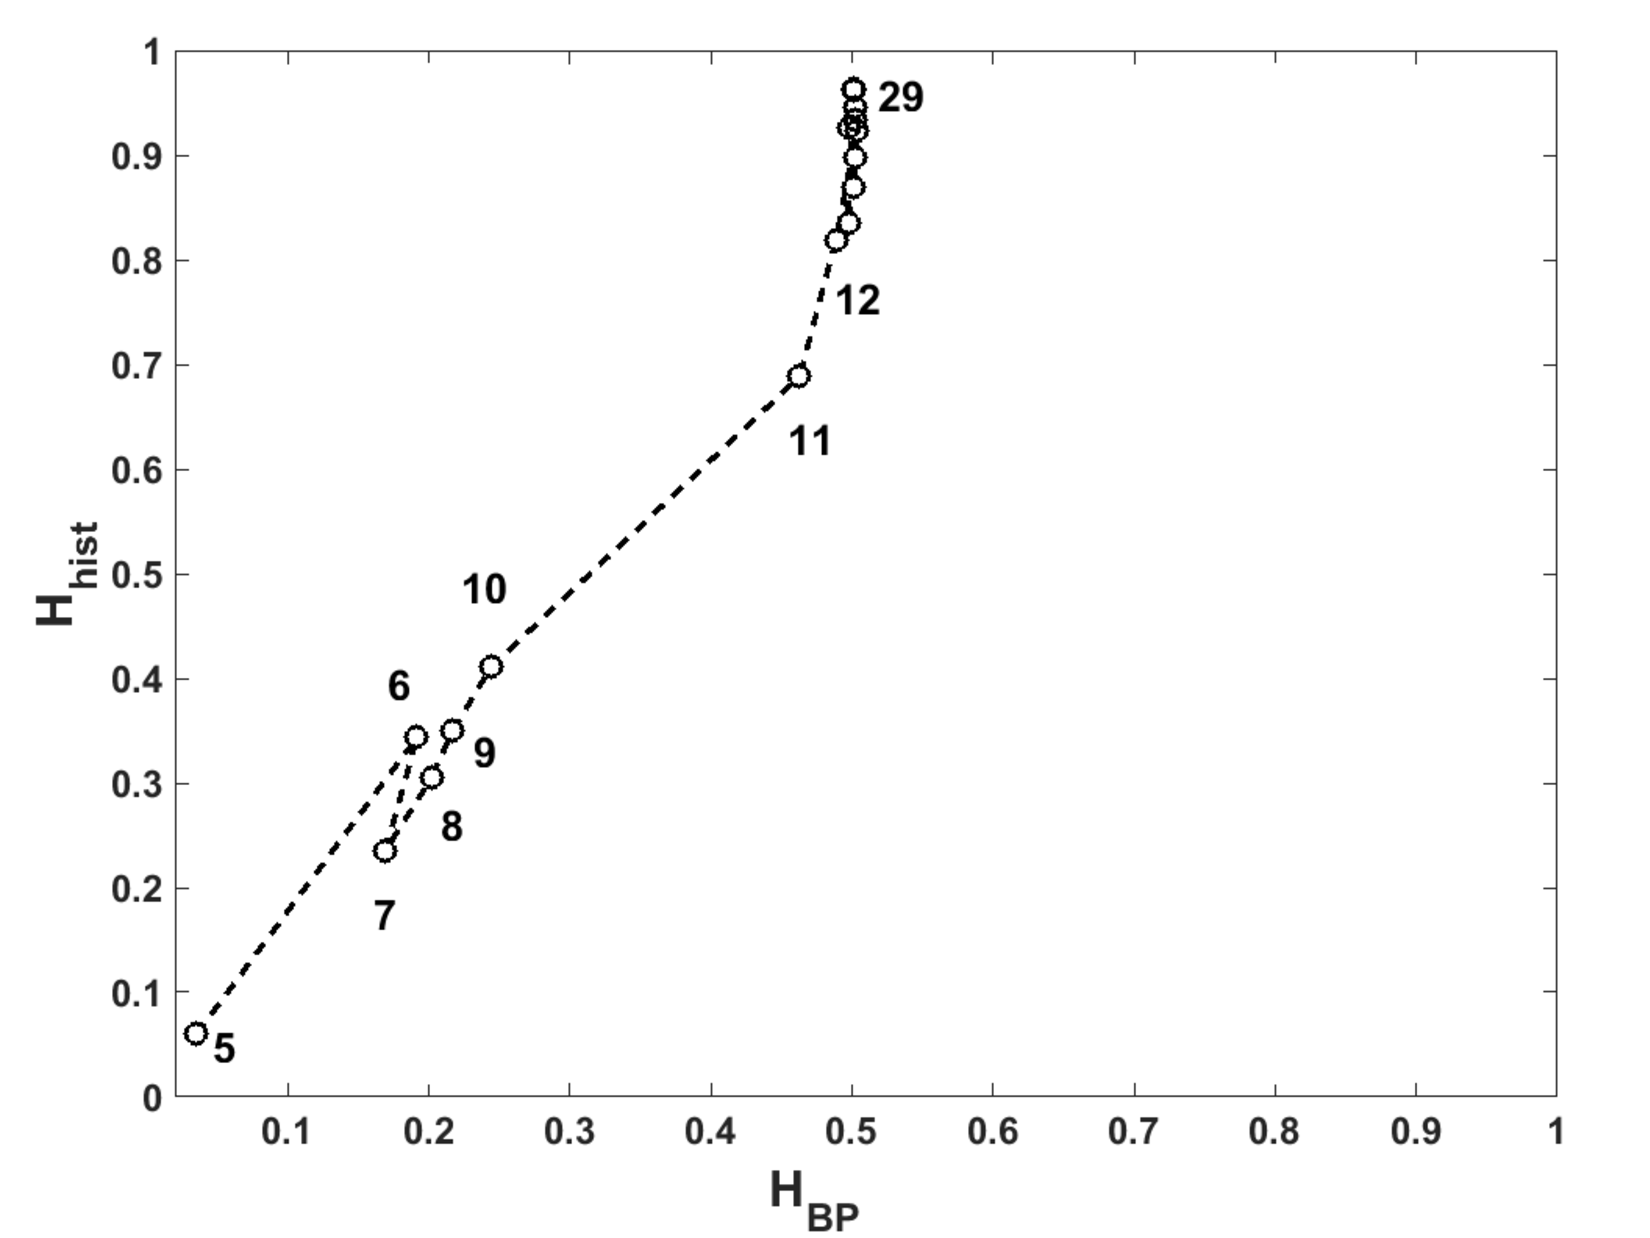
\includegraphics[width=0.85\columnwidth]{HBPvsHhistO}\\
	\caption{Plano $H_{hist}$ - $H_{BP}$ para diferentes números de bits. }\label{fig:HBPvsHhist}
\end{figure}

El plano $H_{hist}$ vs $H_{BP}$, que se muestra en la Figura \ref{fig:HBPvsHhist}, permite una visualización rápida del comportamiento en términos de aleatoriedad del sistema.
Como se dijo, en este plano el punto ``ideal'', desde el punto de vista estadístico, es $(1,1)$.
Aquí, el sistema parece estabilizarse para $n_f$ superior a $12$.
Se puede observar que mientras $H_{hist}$ se estabiliza cerca del valor máximo ($ H_{hist} = 1 $), el $H_{BP}$ tiende a estabilizarse a $0.5$.
Este valor de $ H_{BP} $ es característico de los sistemas caóticos y se debe a las ya mencionadas estructuras internas de sus atractores.

Un resumen del análisis observado de estos resultados se puede ver en la Figura \ref{puntos}.
%
\begin{figure}
	\centering
	\begin{subfigure}[b]{0.49\textwidth}
		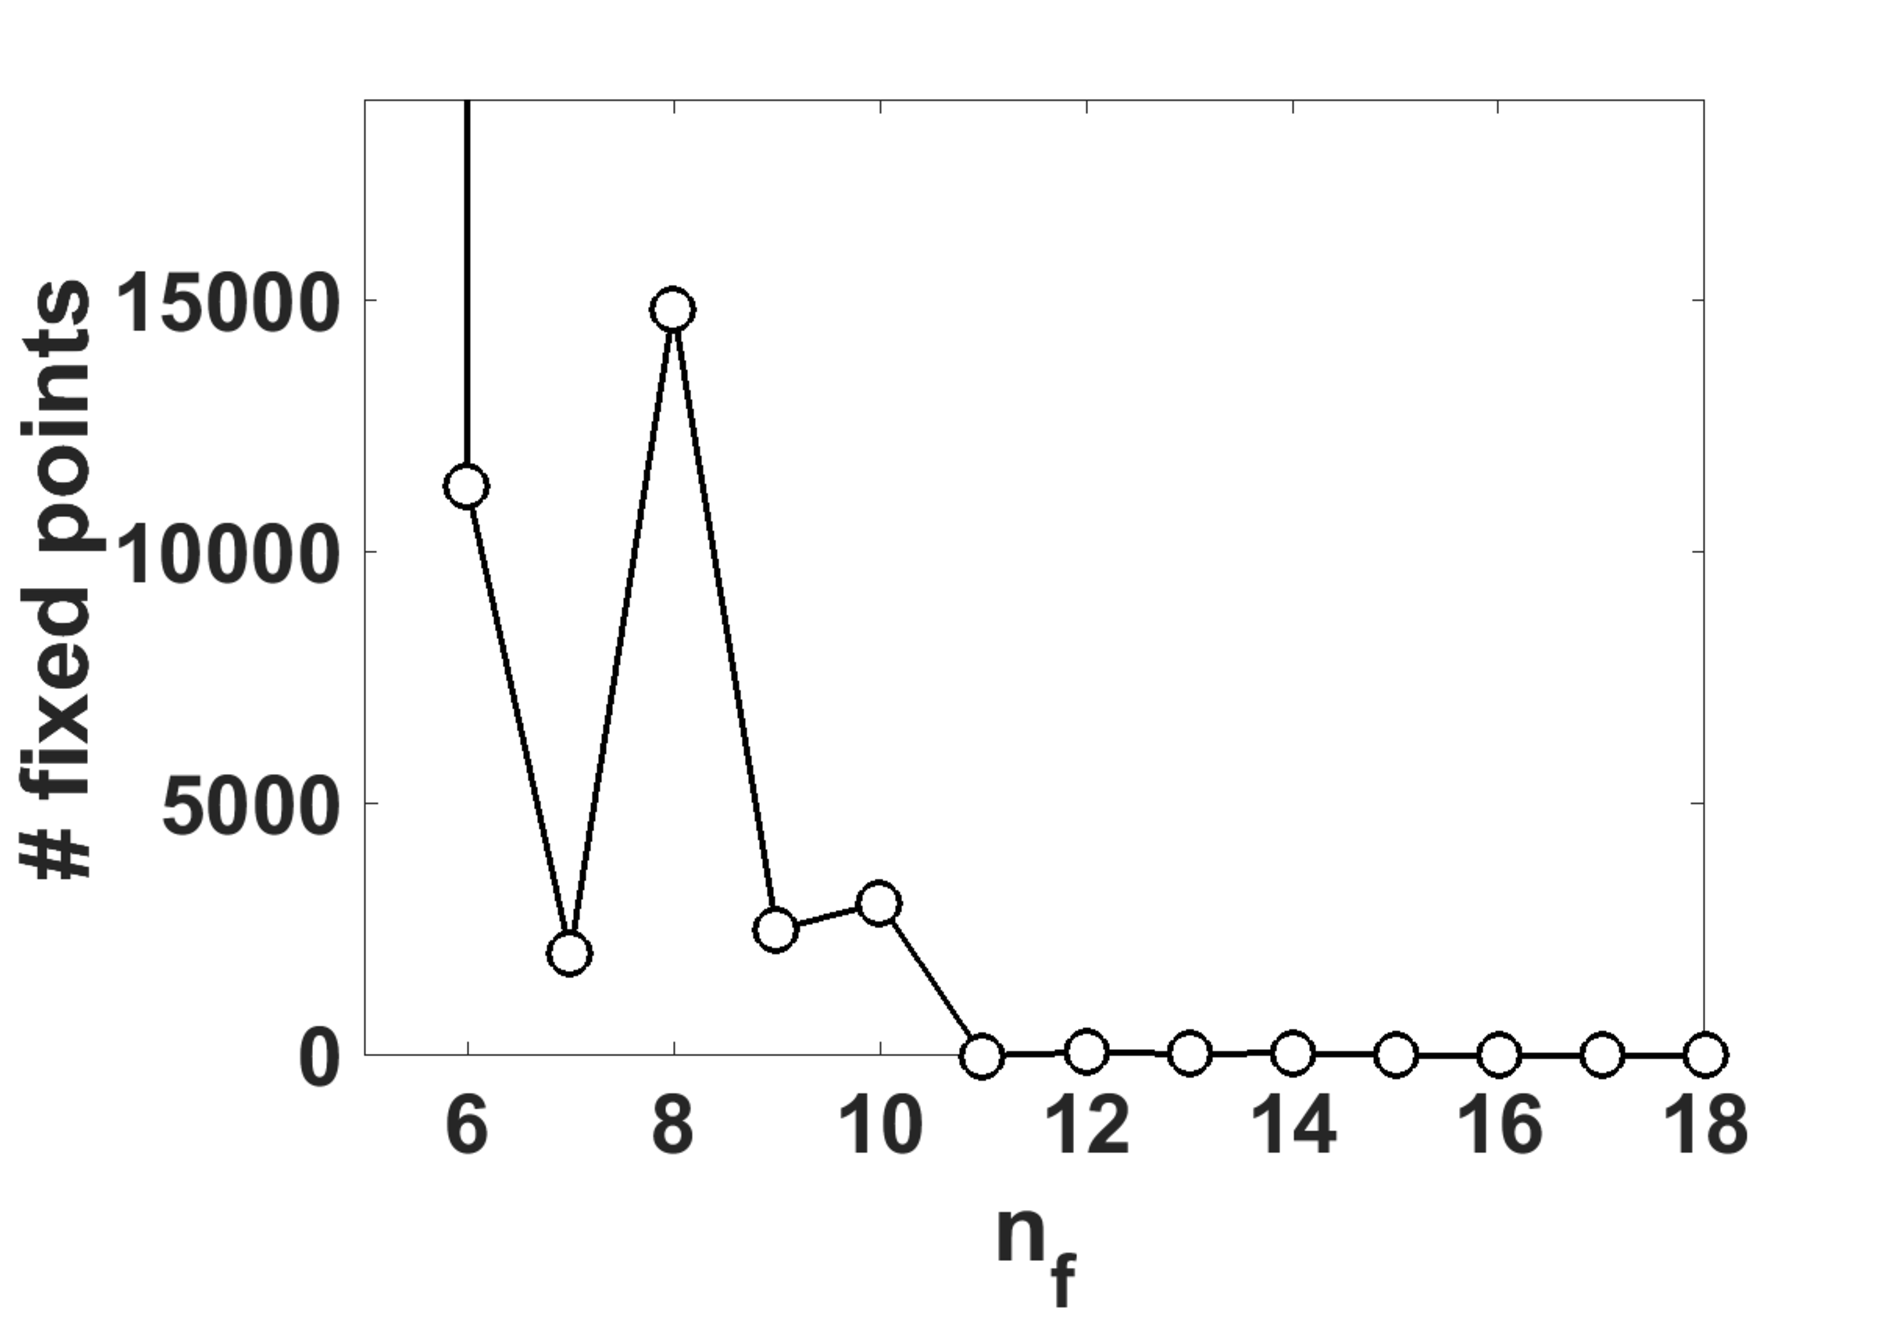
\includegraphics[width=\textwidth]{ptosfijosO}
		\caption{Número de puntos fijos.}
	\end{subfigure}
	\hfill 
	\begin{subfigure}[b]{0.49\textwidth}
		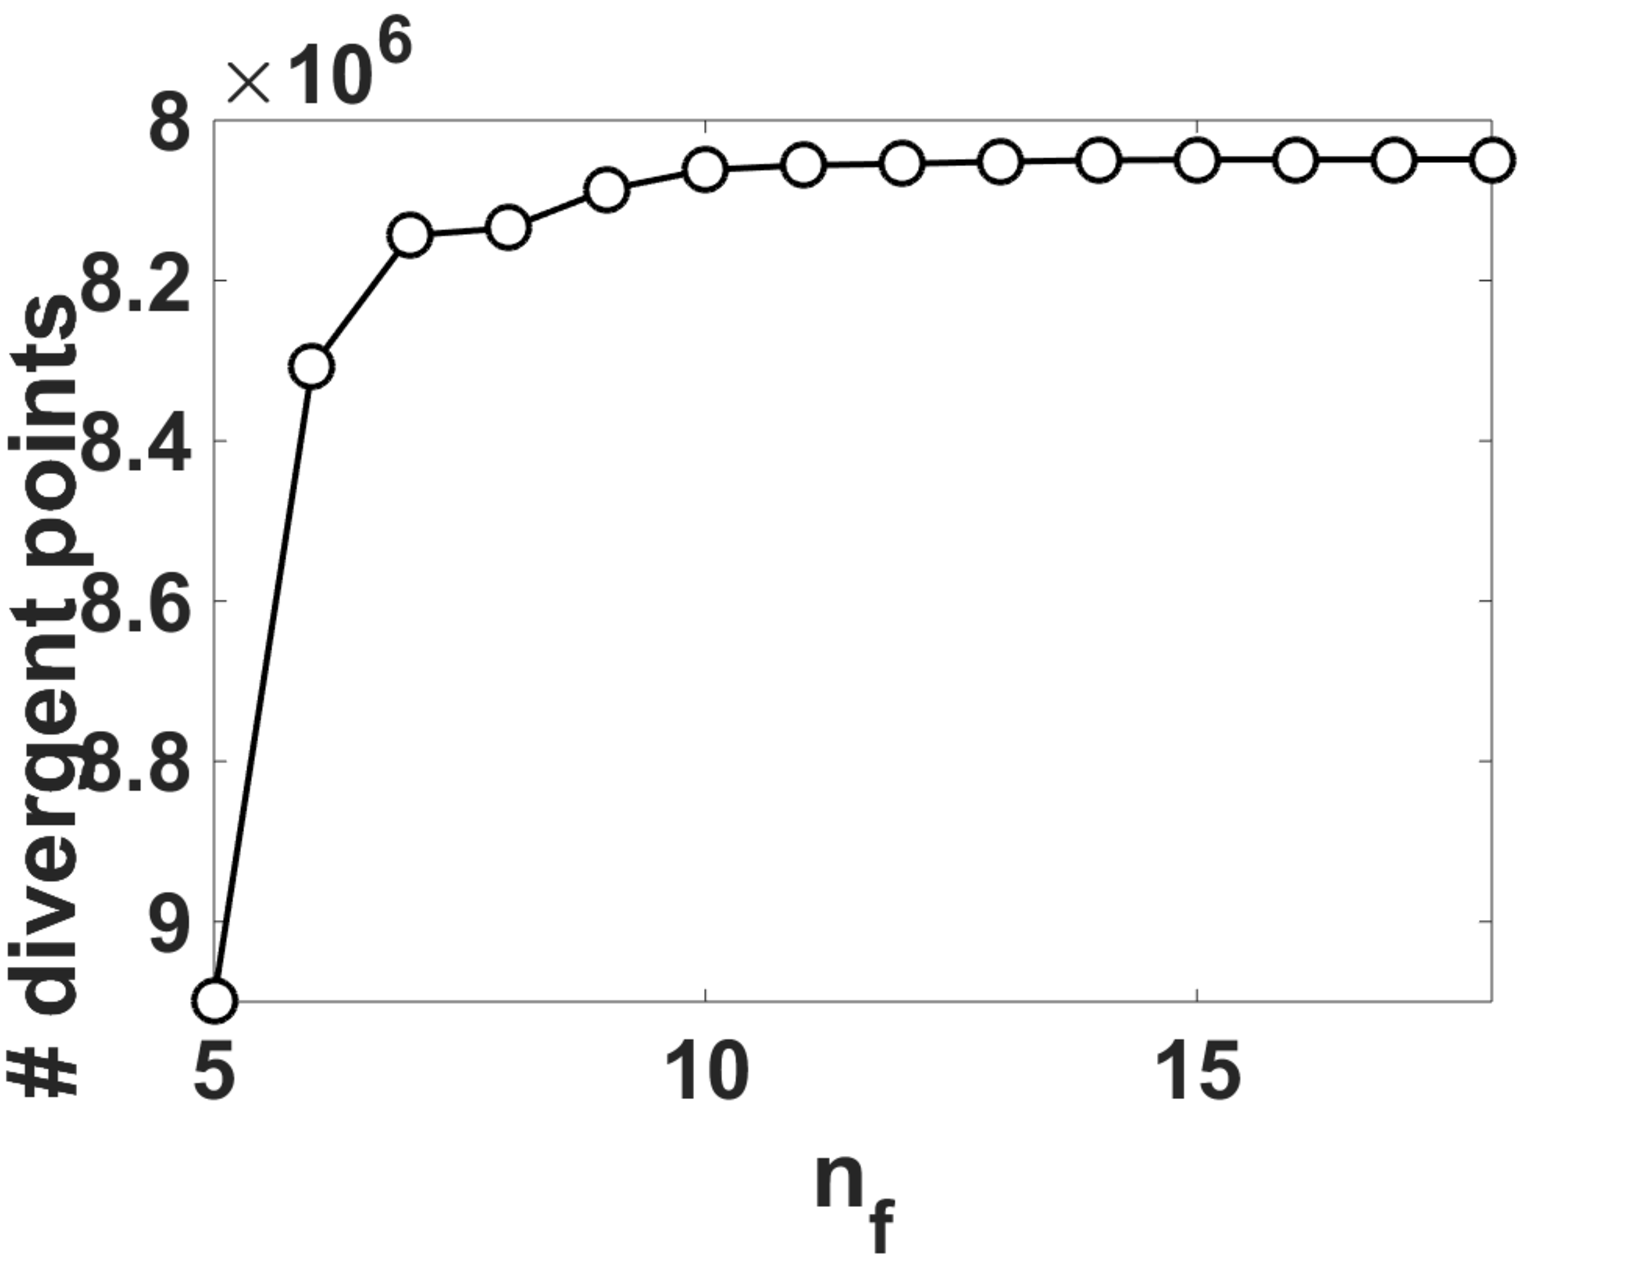
\includegraphics[width=\textwidth]{divergenO}
		\caption{Número de puntos divergentes.}
	\end{subfigure}
	\hfill 
	\begin{subfigure}[b]{0.49\textwidth}
		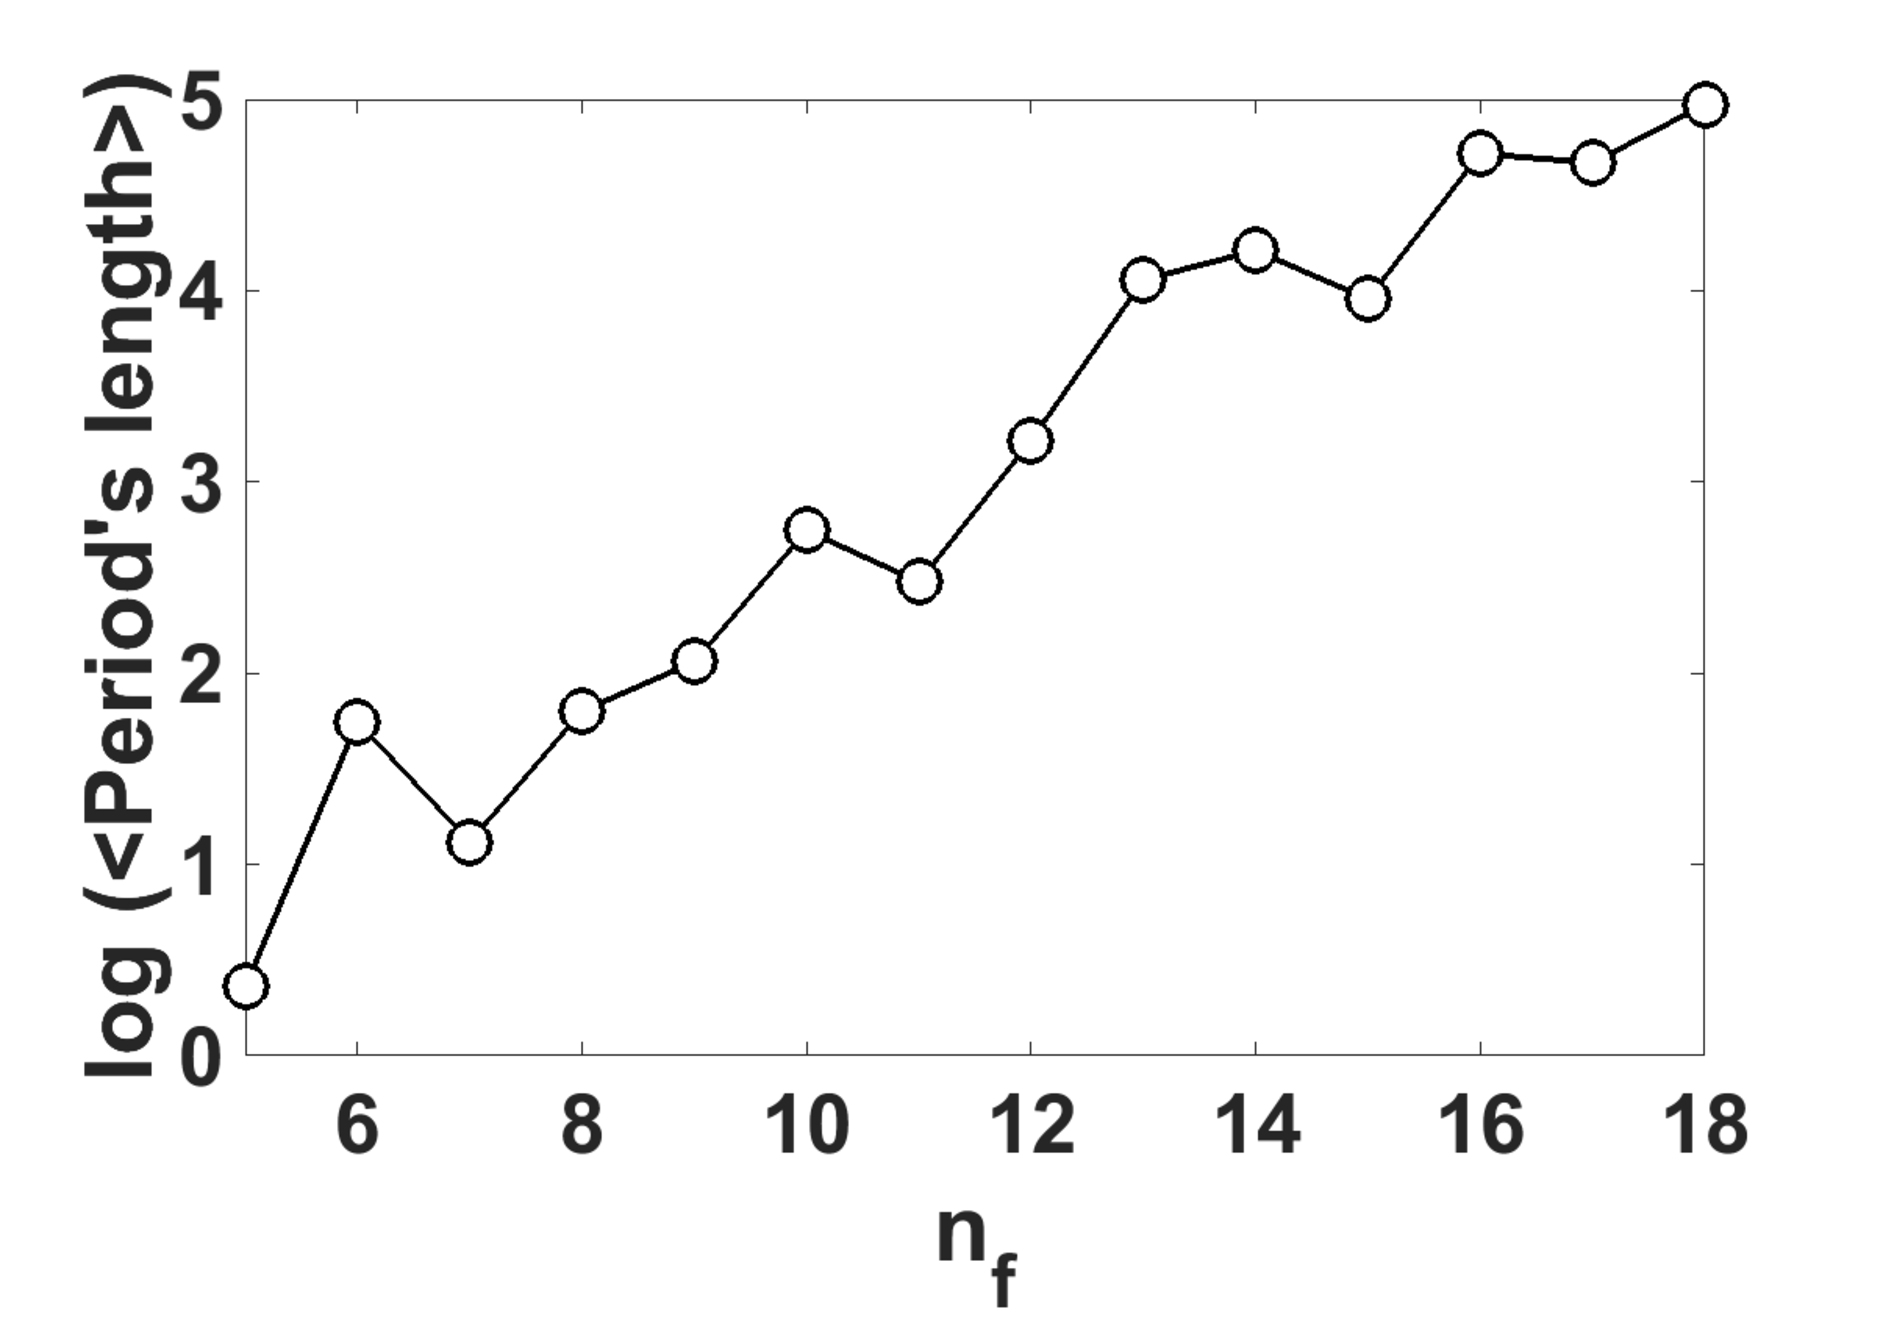
\includegraphics[width=\textwidth]{Periodos_promO}
		\caption{Logaritmo de las longitudes pesadas de ciclos medios.}
	\end{subfigure}
	\hfill   
	\begin{subfigure}[b]{0.49\textwidth}
		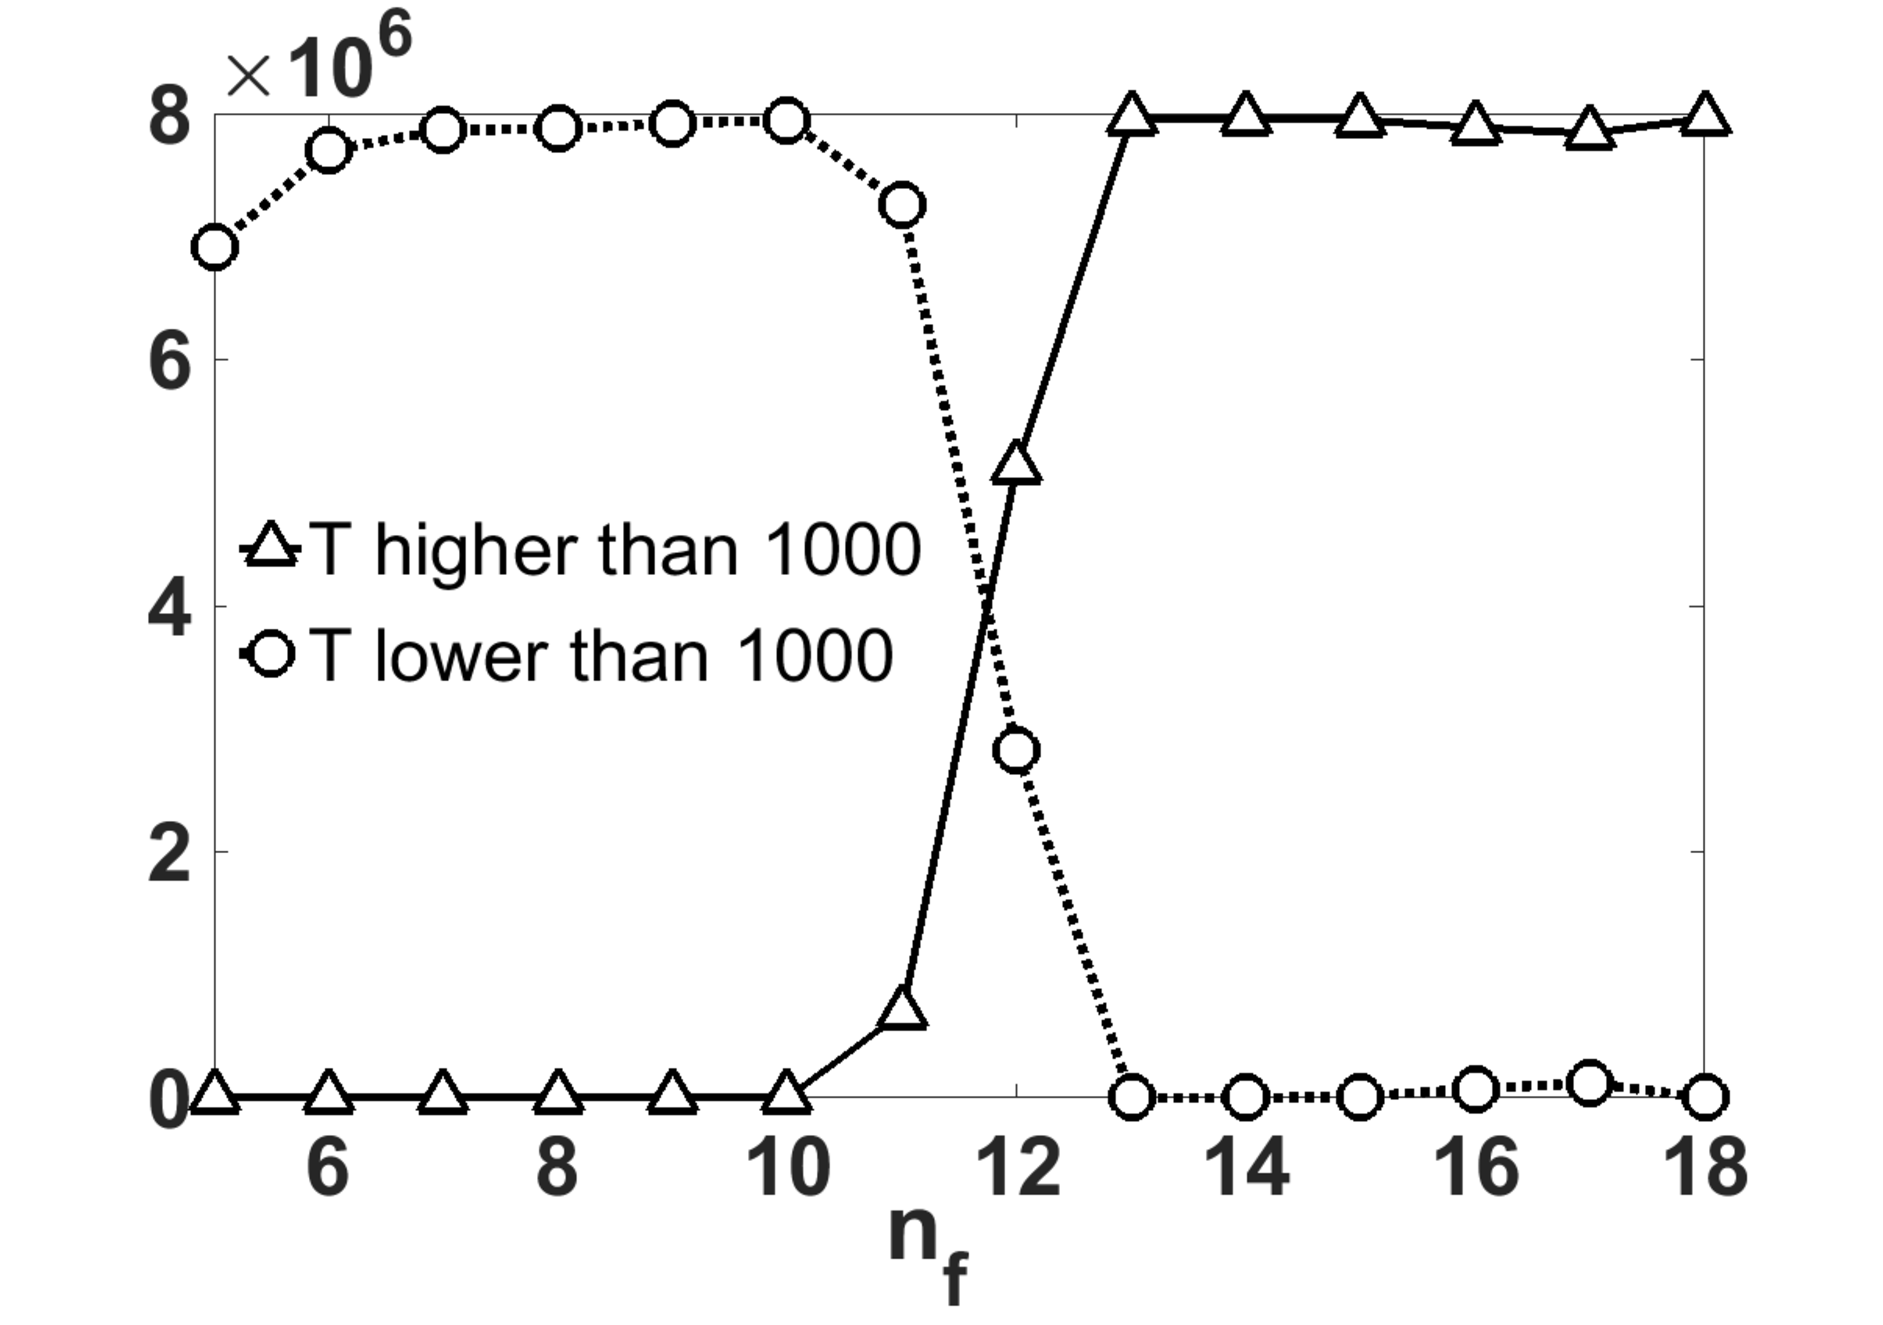
\includegraphics[width=\textwidth]{PuntosO}
		\caption{CIs con longitudes de período mayores y menores que $1~000$.}
	\end{subfigure}
	\caption{Comportamiento de las condiciones iniciales.}\label{puntos}
\end{figure}
%
La Figura \ref{puntos}.a y \ref{puntos}.b muestran el número de puntos que divergen y convergen en puntos fijos respectivamente a medida que aumenta el valor de $n_f$, en ambos casos, el valor final tiende al que se obtiene en implementación en punto flotante.
De estas Figuras se desprende que para $n_f \sim 12$ el sistema parece haberse estabilizado.
La Figura \ref{puntos}.c muestra que el período promediado aumenta a una velocidad logarítmica.
Finalmente, la Figura \ref{puntos}.d muestra el número de condiciones iniciales que presentan períodos $T$ más altos y más bajos que $1~000$.
De nuevo, un valor de $12$ para $n_f$ parece ser el límite para obtener una buena aproximación del sistema.

La Figura \ref{fig:HBPHhist} muestra el promedio ponderado de los cuantificadores $H_{hist}$, $H_{BP}$ y \textsl{MLE}.
En la Figura se puede ver que los tres cuantificadores tienden al valor calculado usando aritmética de punto flotante.
Mientras $H_{BP}$ y \textsl{MLE} se estabilizan para $n_f \sim 12$ o $13$, $H_{hist}$ alcanza el valor en coma flotante de $n_f \sim 19$, mostrando que hay propiedades de las secuencias de salida que sólo este cuantificador puede detectar.
Esto confirma la necesidad de usar ambos cuantificadores para caracterizar la aleatoriedad de las secuencias.
%
\begin{figure}
	\centering
	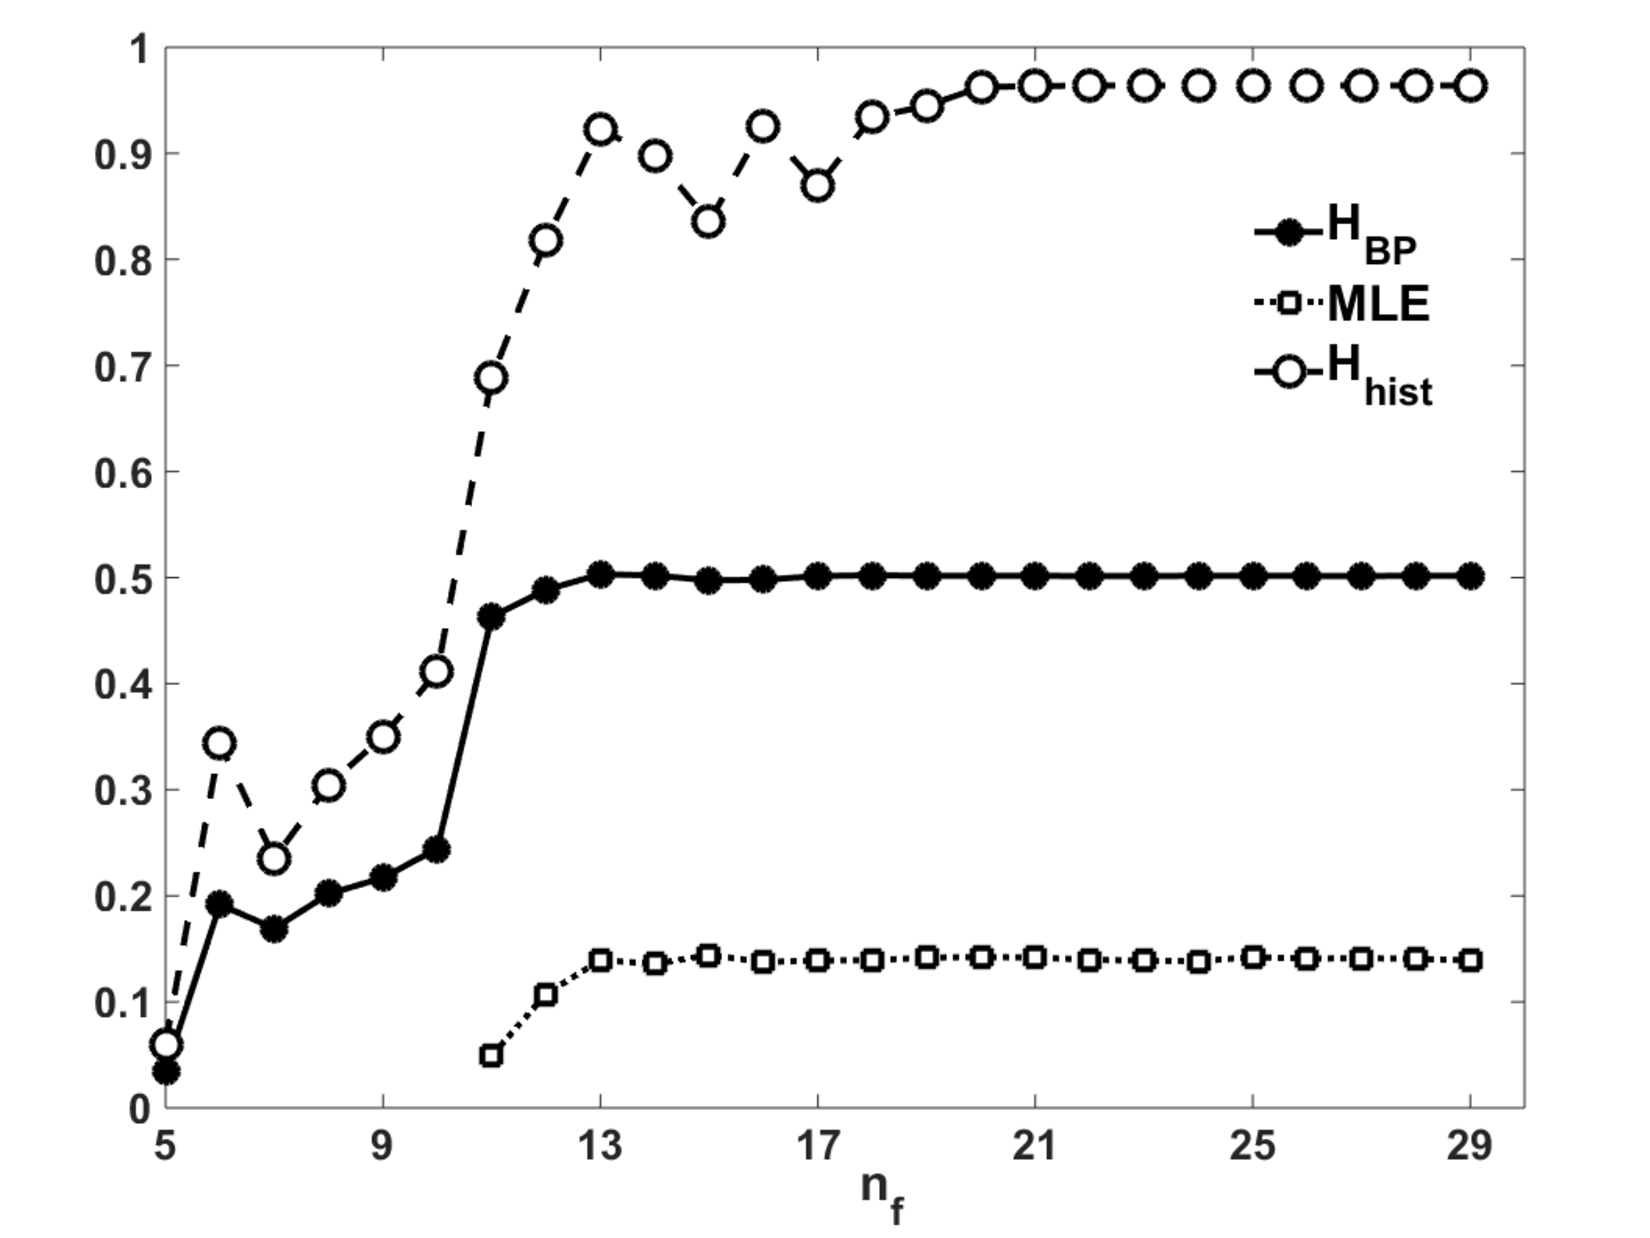
\includegraphics[width=0.75\columnwidth]{HBPHhistO}\\
	\caption{Promedio pesado de cuantificadores $H_{BP}$,  $H_{hist}$ y MLE en función del número de bits.}\label{fig:HBPHhist}
\end{figure}

Como puede verse en el análisis anterior, el número mínimo de bits está determinado por $H_{hist}$ y los resultados son $n_f = 19$ más la cantidad de bits utilizados para representar la parte entera $n_i = 4$, por lo tanto $n_{min}$ resulta ser igual a $23$.
